% Created 2020-09-22 二 18:20
% Intended LaTeX compiler: pdflatex
\documentclass[11pt]{article}
\usepackage[utf8]{inputenc}
\usepackage[T1]{fontenc}
\usepackage{graphicx}
\usepackage{grffile}
\usepackage{longtable}
\usepackage{wrapfig}
\usepackage{rotating}
\usepackage[normalem]{ulem}
\usepackage{amsmath}
\usepackage{textcomp}
\usepackage{amssymb}
\usepackage{capt-of}
\usepackage{hyperref}
\usepackage{minted}
%%%%%%%%%%%%%%%%%%%%%%%%%%%%%%%%%%%%%%
%% TIPS                                 %%
%%%%%%%%%%%%%%%%%%%%%%%%%%%%%%%%%%%%%%
% \substack{a\\b} for multiple lines text

\usepackage[utf8]{inputenc}

\usepackage[B1,T1]{fontenc}

% pdfplots will load xolor automatically without option
\usepackage[dvipsnames]{xcolor}
%%%%%%%%%%%%%%%%%%%%%%%%%%%%%%%%%%%%%%%
%% MATH related pacakge                  %%
%%%%%%%%%%%%%%%%%%%%%%%%%%%%%%%%%%%%%%%
% \usepackage{amsmath} mathtools loads the amsmath
\usepackage{amsmath}
\usepackage{mathtools}


\usepackage{amsthm}
\usepackage{amsbsy}

%\usepackage{commath}

\usepackage{amssymb}
\usepackage{mathrsfs}
%\usepackage{mathabx}
\usepackage{stmaryrd}
\usepackage{empheq}

\usepackage{scalerel}
\usepackage{stackengine}
\usepackage{stackrel}

\usepackage{nicematrix}
\usepackage{tensor}
\usepackage{blkarray}
\usepackage{siunitx}
\usepackage[f]{esvect}

\usepackage{unicode-math}
\setmainfont{TeX Gyre Pagella}
% \setmathfont{STIX}
% \setmathfont{texgyrepagella-math.otf}
% \setmathfont{Libertinus Math}
\setmathfont{Latin Modern Math}
\setmathfont[range={\mscra,\mscrb,\mscrc,\mscrd,\mscre,\mscrf,\mscrg,\mscrh,\mscri,\mscrj,\mscrk,\mscrl,\mscrm,\mscrn,\mscro,\mscrp,\mscrq,\mscrr,\mscrs,\mscrt,\mscru,\mscrv,\mscrw,\mscrx,\mscry,\mscrz,\mscrA,\mscrB,\mscrC,\mscrD,\mscrE,\mscrF,\mscrG,\mscrH,\mscrI,\mscrJ,\mscrK,\mscrL,\mscrM,\mscrN,\mscrO,\mscrP,\mscrQ,\mscrR,\mscrS,\mscrT,\mscrU,\mscrV,\mscrW,\mscrX,\mscrY,\mscrZ}]{Latin Modern Math}
\setmathfont[range={\smwhtdiamond,\enclosediamond,\varlrtriangle}]{Latin Modern Math}
\setmathfont[range={\rightrightarrows,\twoheadrightarrow,\leftrightsquigarrow,\triangledown}]{XITS Math}
\setmathfont[range={\int,\setminus}]{Libertinus Math}



%%%%%%%%%%%%%%%%%%%%%%%%%%%%%%%%%%%%%%%
%% TIKZ related packages                 %%
%%%%%%%%%%%%%%%%%%%%%%%%%%%%%%%%%%%%%%%

\usepackage{pgfplots}
\pgfplotsset{compat=1.15}
\usepackage{tikz}
\usepackage{tikz-cd}
\usepackage{tikz-qtree}

\usetikzlibrary{arrows,positioning,calc,fadings,decorations,matrix,decorations,shapes.misc}
%setting from geogebra
\definecolor{ccqqqq}{rgb}{0.8,0,0}


%%%%%%%%%%%%%%%%%%%%%%%%%%%%%%%%%%%%%%%
%% MISCLELLANEOUS packages               %%
%%%%%%%%%%%%%%%%%%%%%%%%%%%%%%%%%%%%%%%
\usepackage[most]{tcolorbox}
\usepackage{threeparttable}
\usepackage{tabularx}

\usepackage{enumitem}

% wrong with preview
\usepackage{subcaption}
\usepackage{caption}
% {\aunclfamily\Huge}
\usepackage{auncial}

\usepackage{float}

\usepackage{fancyhdr}

\usepackage{ifthen}
\usepackage{xargs}


\usepackage{imakeidx}
\usepackage{hyperref}
\usepackage{soul}


%\usepackage[xetex]{preview}
%%%%%%%%%%%%%%%%%%%%%%%%%%%%%%%%%%%%%%%
%% USEPACKAGES end                       %%
%%%%%%%%%%%%%%%%%%%%%%%%%%%%%%%%%%%%%%%

% \setlist{nosep}
% \numberwithin{equation}{subsection}
% \fancyhead{} % Clear the headers
% \renewcommand{\headrulewidth}{0pt} % Width of line at top of page
% \fancyhead[R]{\slshape\leftmark} % Mark right [R] of page with Chapter name [\leftmark]
% \pagestyle{fancy} % Set default style for all content pages (not TOC, etc)


% \newlength\shlength
% \newcommand\vect[2][0]{\setlength\shlength{#1pt}%
%   \stackengine{-5.6pt}{$#2$}{\smash{$\kern\shlength%
%     \stackengine{7.55pt}{$\mathchar"017E$}%
%       {\rule{\widthof{$#2$}}{.57pt}\kern.4pt}{O}{r}{F}{F}{L}\kern-\shlength$}}%
%       {O}{c}{F}{T}{S}}


\indexsetup{othercode=\small}
\makeindex[columns=2,options={-s /media/wu/file/stuuudy/notes/index_style.ist},intoc]
\makeatletter
\def\@idxitem{\par\hangindent 0pt}
\makeatother


%\newcounter{dummy} \numberwithin{dummy}{section}
\newtheorem{dummy}{dummy}[section]
\theoremstyle{definition}
\newtheorem{definition}[dummy]{Definition}
\theoremstyle{plain}
\newtheorem{corollary}[dummy]{Corollary}
\newtheorem{lemma}[dummy]{Lemma}
\newtheorem{proposition}[dummy]{Proposition}
\newtheorem{theorem}[dummy]{Theorem}
\theoremstyle{definition}
\newtheorem{examplle}{Example}[section]
\theoremstyle{remark}
\newtheorem*{remark}{Remark}
\newtheorem{exercise}{Exercise}[subsection]
\newtheorem{observation}{Observation}[section]


\newenvironment{claim}[1]{\par\noindent\textbf{Claim:}\space#1}{}

\makeatletter
\DeclareFontFamily{U}{tipa}{}
\DeclareFontShape{U}{tipa}{m}{n}{<->tipa10}{}
\newcommand{\arc@char}{{\usefont{U}{tipa}{m}{n}\symbol{62}}}%

\newcommand{\arc}[1]{\mathpalette\arc@arc{#1}}

\newcommand{\arc@arc}[2]{%
  \sbox0{$\m@th#1#2$}%
  \vbox{
    \hbox{\resizebox{\wd0}{\height}{\arc@char}}
    \nointerlineskip
    \box0
  }%
}
\makeatother

\setcounter{MaxMatrixCols}{20}
%%%%%%% ABS
\DeclarePairedDelimiter\abss{\lvert}{\rvert}%
\DeclarePairedDelimiter\normm{\lVert}{\rVert}%

% Swap the definition of \abs* and \norm*, so that \abs
% and \norm resizes the size of the brackets, and the
% starred version does not.
\makeatletter
\let\oldabs\abss
%\def\abs{\@ifstar{\oldabs}{\oldabs*}}
\newcommand{\abs}{\@ifstar{\oldabs}{\oldabs*}}
\newcommand{\norm}[1]{\left\lVert#1\right\rVert}
%\let\oldnorm\normm
%\def\norm{\@ifstar{\oldnorm}{\oldnorm*}}
%\renewcommand{norm}{\@ifstar{\oldnorm}{\oldnorm*}}
\makeatother

% \newcommand\what[1]{\ThisStyle{%
%     \setbox0=\hbox{$\SavedStyle#1$}%
%     \stackengine{-1.0\ht0+.5pt}{$\SavedStyle#1$}{%
%       \stretchto{\scaleto{\SavedStyle\mkern.15mu\char'136}{2.6\wd0}}{1.4\ht0}%
%     }{O}{c}{F}{T}{S}%
%   }
% }

% \newcommand\wtilde[1]{\ThisStyle{%
%     \setbox0=\hbox{$\SavedStyle#1$}%
%     \stackengine{-.1\LMpt}{$\SavedStyle#1$}{%
%       \stretchto{\scaleto{\SavedStyle\mkern.2mu\AC}{.5150\wd0}}{.6\ht0}%
%     }{O}{c}{F}{T}{S}%
%   }
% }

% \newcommand\wbar[1]{\ThisStyle{%
%     \setbox0=\hbox{$\SavedStyle#1$}%
%     \stackengine{.5pt+\LMpt}{$\SavedStyle#1$}{%
%       \rule{\wd0}{\dimexpr.3\LMpt+.3pt}%
%     }{O}{c}{F}{T}{S}%
%   }
% }

\newcommand{\bl}[1] {\boldsymbol{#1}}
\newcommand{\Wt}[1] {\stackrel{\sim}{\smash{#1}\rule{0pt}{1.1ex}}}
\newcommand{\wt}[1] {\widetilde{#1}}
\newcommand{\tf}[1] {\textbf{#1}}


%For boxed texts in align, use Aboxed{}
%otherwise use boxed{}

\DeclareMathSymbol{\widehatsym}{\mathord}{largesymbols}{"62}
\newcommand\lowerwidehatsym{%
  \text{\smash{\raisebox{-1.3ex}{%
    $\widehatsym$}}}}
\newcommand\fixwidehat[1]{%
  \mathchoice
    {\accentset{\displaystyle\lowerwidehatsym}{#1}}
    {\accentset{\textstyle\lowerwidehatsym}{#1}}
    {\accentset{\scriptstyle\lowerwidehatsym}{#1}}
    {\accentset{\scriptscriptstyle\lowerwidehatsym}{#1}}
  }


\newcommand{\cupdot}{\mathbin{\dot{\cup}}}
\newcommand{\bigcupdot}{\mathop{\dot{\bigcup}}}

\usepackage{graphicx}

\usepackage[toc,page]{appendix}

% text on arrow for xRightarrow
\makeatletter
%\newcommand{\xRightarrow}[2][]{\ext@arrow 0359\Rightarrowfill@{#1}{#2}}
\makeatother

% Arbitrary long arrow
\newcommand{\Rarrow}[1]{%
\parbox{#1}{\tikz{\draw[->](0,0)--(#1,0);}}
}

\newcommand{\LRarrow}[1]{%
\parbox{#1}{\tikz{\draw[<->](0,0)--(#1,0);}}
}


\makeatletter
\providecommand*{\rmodels}{%
  \mathrel{%
    \mathpalette\@rmodels\models
  }%
}
\newcommand*{\@rmodels}[2]{%
  \reflectbox{$\m@th#1#2$}%
}
\makeatother







\newcommand{\trcl}[1]{%
  \mathrm{trcl}{(#1)}
}



% Roman numerals
\makeatletter
\newcommand*{\rom}[1]{\expandafter\@slowromancap\romannumeral #1@}
\makeatother
% \\def \\b\([a-zA-Z]\) {\\boldsymbol{[a-zA-z]}}
% \\DeclareMathOperator{\\b\1}{\\textbf{\1}}


\DeclareMathOperator{\bx}{\textbf{x}}
\DeclareMathOperator{\bz}{\textbf{z}}
\DeclareMathOperator{\bff}{\textbf{f}}
\DeclareMathOperator{\ba}{\textbf{a}}
\DeclareMathOperator{\bk}{\textbf{k}}
\DeclareMathOperator{\bs}{\textbf{s}}
\DeclareMathOperator{\bh}{\textbf{h}}
\DeclareMathOperator{\bc}{\textbf{c}}
\DeclareMathOperator{\br}{\textbf{r}}
\DeclareMathOperator{\bi}{\textbf{i}}
\DeclareMathOperator{\bj}{\textbf{j}}
\DeclareMathOperator{\bn}{\textbf{n}}
\DeclareMathOperator{\be}{\textbf{e}}
\DeclareMathOperator{\bo}{\textbf{o}}
\DeclareMathOperator{\bU}{\textbf{U}}
\DeclareMathOperator{\bL}{\textbf{L}}
\DeclareMathOperator{\bV}{\textbf{V}}
\def \bzero {\mathbf{0}}
\def \btwo {\mathbf{2}}
\DeclareMathOperator{\bv}{\textbf{v}}
\DeclareMathOperator{\bp}{\textbf{p}}
\DeclareMathOperator{\bI}{\textbf{I}}
\DeclareMathOperator{\bM}{\textbf{M}}
\DeclareMathOperator{\bN}{\textbf{N}}
\DeclareMathOperator{\bK}{\textbf{K}}
\DeclareMathOperator{\bt}{\textbf{t}}
\DeclareMathOperator{\bb}{\textbf{b}}
\DeclareMathOperator{\bA}{\textbf{A}}
\DeclareMathOperator{\bX}{\textbf{X}}
\DeclareMathOperator{\bu}{\textbf{u}}
\DeclareMathOperator{\bS}{\textbf{S}}
\DeclareMathOperator{\bZ}{\textbf{Z}}
\DeclareMathOperator{\by}{\textbf{y}}
\DeclareMathOperator{\bw}{\textbf{w}}
\DeclareMathOperator{\bT}{\textbf{T}}
\DeclareMathOperator{\bF}{\textbf{F}}
\DeclareMathOperator{\bmm}{\textbf{m}}
\DeclareMathOperator{\bW}{\textbf{W}}
\DeclareMathOperator{\bR}{\textbf{R}}
\DeclareMathOperator{\bC}{\textbf{C}}
\DeclareMathOperator{\bD}{\textbf{D}}
\DeclareMathOperator{\bE}{\textbf{E}}
\DeclareMathOperator{\bQ}{\textbf{Q}}
\DeclareMathOperator{\bP}{\textbf{P}}
\DeclareMathOperator{\bY}{\textbf{Y}}
\DeclareMathOperator{\bH}{\textbf{H}}
\DeclareMathOperator{\bB}{\textbf{B}}
\DeclareMathOperator{\bG}{\textbf{G}}
\def \blambda {\symbf{\lambda}}
\def \boldeta {\symbf{\eta}}
\def \balpha {\symbf{\alpha}}
\def \bbeta {\symbf{\beta}}
\def \bgamma {\symbf{\gamma}}
\def \bxi {\symbf{\xi}}
\def \bLambda {\symbf{\Lambda}}

\newcommand{\bto}{{\boldsymbol{\to}}}
\newcommand{\Ra}{\Rightarrow}
\newcommand\und[1]{\underline{#1}}
\def \bPhi {\boldsymbol{\Phi}}
\def \btheta {\boldsymbol{\theta}}
\def \bTheta {\boldsymbol{\Theta}}
\def \bmu {\boldsymbol{\mu}}
\def \bphi {\boldsymbol{\phi}}
\def \bSigma {\boldsymbol{\Sigma}}
\def \lb {\left\{}
\def \rb {\right\}}
\def \la {\langle}
\def \ra {\rangle}
\def \caln {\mathcal{N}}
\def \dissum {\displaystyle\Sigma}
\def \dispro {\displaystyle\prod}
\def \E {\mathbb{E}}
\def \Q {\mathbb{Q}}
\def \N {\mathbb{N}}
\def \V {\mathbb{V}}
\def \R {\mathbb{R}}
\def \P {\mathbb{P}}
\def \A {\mathbb{A}}
\def \F {\mathbb{F}}
\def \Z {\mathbb{Z}}
\def \I {\mathbb{I}}
\def \C {\mathbb{C}}
\def \cala {\mathcal{A}}
\def \cale {\mathcal{E}}
\def \calb {\mathcal{B}}
\def \calq {\mathcal{Q}}
\def \calp {\mathcal{P}}
\def \cals {\mathcal{S}}
\def \calx {\mathcal{X}}
\def \caly {\mathcal{Y}}
\def \calg {\mathcal{G}}
\def \cald {\mathcal{D}}
\def \caln {\mathcal{N}}
\def \calr {\mathcal{R}}
\def \calt {\mathcal{T}}
\def \calm {\mathcal{M}}
\def \calw {\mathcal{W}}
\def \calc {\mathcal{C}}
\def \calv {\mathcal{V}}
\def \calf {\mathcal{F}}
\def \calk {\mathcal{K}}
\def \call {\mathcal{L}}
\def \calu {\mathcal{U}}
\def \calo {\mathcal{O}}
\def \calh {\mathcal{H}}
\def \cali {\mathcal{I}}

\def \bcup {\bigcup}

% set theory

\def \zfcc {\textbf{ZFC}^-}
\def \ac  {\textbf{AC}}
\def \gl  {\textbf{L }}
\def \gll {\textbf{L}}
\newcommand{\zfm}{$\textbf{ZF}^-$}

%\def \zfm {$\textbf{ZF}^-$}
\def \zfmm {\textbf{ZF}^-}
\def \wf {\textbf{WF }}
\def \on {\textbf{On }}
\def \cm {\textbf{M }}
\def \cn {\textbf{N }}
\def \cv {\textbf{V }}
\def \zc {\textbf{ZC }}
\def \zcm {\textbf{ZC}}
\def \zff {\textbf{ZF}}
\def \wfm {\textbf{WF}}
\def \onm {\textbf{On}}
\def \cmm {\textbf{M}}
\def \cnm {\textbf{N}}
\def \cvm {\textbf{V}}
\def \gchh {\textbf{GCH}}
\renewcommand{\restriction}{\mathord{\upharpoonright}}
\def \pred {\text{pred}}

\def \rank {\text{rank}}
\def \con {\text{Con}}
\def \deff {\text{Def}}


\def \uin {\underline{\in}}
\def \oin {\overline{\in}}
\def \uR {\underline{R}}
\def \oR {\overline{R}}
\def \uP {\underline{P}}
\def \oP {\overline{P}}

\def \Ra {\Rightarrow}

\def \e {\enspace}

\def \sgn {\operatorname{sgn}}
\def \gen {\operatorname{gen}}
\def \Hom {\operatorname{Hom}}
\def \hom {\operatorname{hom}}
\def \Sub {\operatorname{Sub}}

\def \supp {\operatorname{supp}}

\def \epiarrow {\twoheadarrow}
\def \monoarrow {\rightarrowtail}
\def \rrarrow {\rightrightarrows}

% \def \minus {\text{-}}
% \newcommand{\minus}{\scalebox{0.75}[1.0]{$-$}}
% \DeclareUnicodeCharacter{002D}{\minus}


\def \tril {\triangleleft}

\def \ACF {\text{ACF}}
\def \GL {\text{GL}}
\def \PGL {\text{PGL}}
\def \equal {=}
\def \deg {\text{deg}}
\def \degree {\text{degree}}
\def \app {\text{App}}
\def \FV {\text{FV}}
\def \conv {\text{conv}}
\def \cont {\text{cont}}
\DeclareMathOperator{\cl}{\textbf{CL}}
\DeclareMathOperator{\sg}{sg}
\DeclareMathOperator{\trdeg}{trdeg}
\def \Ord {\text{Ord}}

\DeclareMathOperator{\cf}{cf}
\DeclareMathOperator{\zfc}{ZFC}

%\DeclareMathOperator{\Th}{Th}
%\def \th {\text{Th}}
% \newcommand{\th}{\text{Th}}
\DeclareMathOperator{\type}{type}
\DeclareMathOperator{\zf}{\textbf{ZF}}
\def \fa {\mathfrak{a}}
\def \fb {\mathfrak{b}}
\def \fc {\mathfrak{c}}
\def \fd {\mathfrak{d}}
\def \fe {\mathfrak{e}}
\def \ff {\mathfrak{f}}
\def \fg {\mathfrak{g}}
\def \fh {\mathfrak{h}}
%\def \fi {\mathfrak{i}}
\def \fj {\mathfrak{j}}
\def \fk {\mathfrak{k}}
\def \fl {\mathfrak{l}}
\def \fm {\mathfrak{m}}
\def \fn {\mathfrak{n}}
\def \fo {\mathfrak{o}}
\def \fp {\mathfrak{p}}
\def \fq {\mathfrak{q}}
\def \fr {\mathfrak{r}}
\def \fs {\mathfrak{s}}
\def \ft {\mathfrak{t}}
\def \fu {\mathfrak{u}}
\def \fv {\mathfrak{v}}
\def \fw {\mathfrak{w}}
\def \fx {\mathfrak{x}}
\def \fy {\mathfrak{y}}
\def \fz {\mathfrak{z}}
\def \fA {\mathfrak{A}}
\def \fB {\mathfrak{B}}
\def \fC {\mathfrak{C}}
\def \fD {\mathfrak{D}}
\def \fE {\mathfrak{E}}
\def \fF {\mathfrak{F}}
\def \fG {\mathfrak{G}}
\def \fH {\mathfrak{H}}
\def \fI {\mathfrak{I}}
\def \fJ {\mathfrak{J}}
\def \fK {\mathfrak{K}}
\def \fL {\mathfrak{L}}
\def \fM {\mathfrak{M}}
\def \fN {\mathfrak{N}}
\def \fO {\mathfrak{O}}
\def \fP {\mathfrak{P}}
\def \fQ {\mathfrak{Q}}
\def \fR {\mathfrak{R}}
\def \fS {\mathfrak{S}}
\def \fT {\mathfrak{T}}
\def \fU {\mathfrak{U}}
\def \fV {\mathfrak{V}}
\def \fW {\mathfrak{W}}
\def \fX {\mathfrak{X}}
\def \fY {\mathfrak{Y}}
\def \fZ {\mathfrak{Z}}

\def \sfA {\textsf{A}}
\def \sfB {\textsf{B}}
\def \sfC {\textsf{C}}
\def \sfD {\textsf{D}}
\def \sfE {\textsf{E}}
\def \sfF {\textsf{F}}
\def \sfG {\textsf{G}}
\def \sfH {\textsf{H}}
\def \sfI {\textsf{I}}
\def \sfj {\textsf{J}}
\def \sfK {\textsf{K}}
\def \sfL {\textsf{L}}
\def \sfM {\textsf{M}}
\def \sfN {\textsf{N}}
\def \sfO {\textsf{O}}
\def \sfP {\textsf{P}}
\def \sfQ {\textsf{Q}}
\def \sfR {\textsf{R}}
\def \sfS {\textsf{S}}
\def \sfT {\textsf{T}}
\def \sfU {\textsf{U}}
\def \sfV {\textsf{V}}
\def \sfW {\textsf{W}}
\def \sfX {\textsf{X}}
\def \sfY {\textsf{Y}}
\def \sfZ {\textsf{Z}}
\def \sfa {\textsf{a}}
\def \sfb {\textsf{b}}
\def \sfc {\textsf{c}}
\def \sfd {\textsf{d}}
\def \sfe {\textsf{e}}
\def \sff {\textsf{f}}
\def \sfg {\textsf{g}}
\def \sfh {\textsf{h}}
\def \sfi {\textsf{i}}
\def \sfj {\textsf{j}}
\def \sfk {\textsf{k}}
\def \sfl {\textsf{l}}
\def \sfm {\textsf{m}}
\def \sfn {\textsf{n}}
\def \sfo {\textsf{o}}
\def \sfp {\textsf{p}}
\def \sfq {\textsf{q}}
\def \sfr {\textsf{r}}
\def \sfs {\textsf{s}}
\def \sft {\textsf{t}}
\def \sfu {\textsf{u}}
\def \sfv {\textsf{v}}
\def \sfw {\textsf{w}}
\def \sfx {\textsf{x}}
\def \sfy {\textsf{y}}
\def \sfz {\textsf{z}}



%\DeclareMathOperator{\ker}{ker}
\DeclareMathOperator{\im}{im}

\DeclareMathOperator{\inn}{Inn}
\DeclareMathOperator{\AC}{\textbf{AC}}
\DeclareMathOperator{\cod}{cod}
\DeclareMathOperator{\dom}{dom}
\DeclareMathOperator{\ran}{ran}
\DeclareMathOperator{\textd}{d}
\DeclareMathOperator{\td}{d}
\DeclareMathOperator{\id}{id}
\DeclareMathOperator{\LT}{LT}
\DeclareMathOperator{\Mat}{Mat}
\DeclareMathOperator{\Eq}{Eq}
\DeclareMathOperator{\irr}{irr}
\DeclareMathOperator{\Fr}{Fr}
\DeclareMathOperator{\Gal}{Gal}
\DeclareMathOperator{\lcm}{lcm}
\DeclareMathOperator{\alg}{\text{alg}}
\DeclareMathOperator{\Th}{Th}

\DeclareMathOperator{\DAG}{DAG}
\DeclareMathOperator{\ODAG}{ODAG}

% \varprod
\DeclareSymbolFont{largesymbolsA}{U}{txexa}{m}{n}
\DeclareMathSymbol{\varprod}{\mathop}{largesymbolsA}{16}
% \DeclareMathSymbol{\tonm}{\boldsymbol{\to}\textbf{Nm}}
\def \tonm {\bto\textbf{Nm}}
\def \tohm {\bto\textbf{Hm}}

% Category theory
\DeclareMathOperator{\Ab}{\textbf{Ab}}
\DeclareMathOperator{\Alg}{\textbf{Alg}}
\DeclareMathOperator{\Rng}{\textbf{Rng}}
\DeclareMathOperator{\Sets}{\textbf{Sets}}
\DeclareMathOperator{\Met}{\textbf{Met}}
\DeclareMathOperator{\Aut}{\textbf{Aut}}
\DeclareMathOperator{\RMod}{R-\textbf{Mod}}
\DeclareMathOperator{\RAlg}{R-\textbf{Alg}}
\DeclareMathOperator{\LF}{LF}
\DeclareMathOperator{\op}{op}
% Model theory
\DeclareMathOperator{\tp}{tp}
\DeclareMathOperator{\Diag}{Diag}
\DeclareMathOperator{\el}{el}
\DeclareMathOperator{\depth}{depth}
\DeclareMathOperator{\FO}{FO}
\DeclareMathOperator{\fin}{fin}
\DeclareMathOperator{\qr}{qr}
\DeclareMathOperator{\Mod}{Mod}
\DeclareMathOperator{\TC}{TC}
\DeclareMathOperator{\KH}{KH}
\DeclareMathOperator{\Part}{Part}
\DeclareMathOperator{\Infset}{\textsf{Infset}}
\DeclareMathOperator{\DLO}{\textsf{DLO}}
\DeclareMathOperator{\sfMod}{\textsf{Mod}}
\DeclareMathOperator{\AbG}{\textsf{AbG}}
\DeclareMathOperator{\sfACF}{\textsf{ACF}}
% Computability Theorem
\DeclareMathOperator{\Tot}{Tot}
\DeclareMathOperator{\graph}{graph}
\DeclareMathOperator{\Fin}{Fin}
\DeclareMathOperator{\Cof}{Cof}
\DeclareMathOperator{\lh}{lh}
% Commutative Algebra
\DeclareMathOperator{\ord}{ord}
\DeclareMathOperator{\Idem}{Idem}
\DeclareMathOperator{\zdiv}{z.div}
\DeclareMathOperator{\Frac}{Frac}
\DeclareMathOperator{\rad}{rad}
\DeclareMathOperator{\nil}{nil}
\DeclareMathOperator{\Ann}{Ann}
\DeclareMathOperator{\End}{End}
\DeclareMathOperator{\coim}{coim}
\DeclareMathOperator{\coker}{coker}
\DeclareMathOperator{\Bil}{Bil}
\DeclareMathOperator{\Tril}{Tril}
% Topology
\newcommand{\interior}[1]{%
  {\kern0pt#1}^{\mathrm{o}}%
}

% \makeatletter
% \newcommand{\vect}[1]{%
%   \vbox{\m@th \ialign {##\crcr
%   \vectfill\crcr\noalign{\kern-\p@ \nointerlineskip}
%   $\hfil\displaystyle{#1}\hfil$\crcr}}}
% \def\vectfill{%
%   $\m@th\smash-\mkern-7mu%
%   \cleaders\hbox{$\mkern-2mu\smash-\mkern-2mu$}\hfill
%   \mkern-7mu\raisebox{-3.81pt}[\p@][\p@]{$\mathord\mathchar"017E$}$}

% \newcommand{\amsvect}{%
%   \mathpalette {\overarrow@\vectfill@}}
% \def\vectfill@{\arrowfill@\relbar\relbar{\raisebox{-3.81pt}[\p@][\p@]{$\mathord\mathchar"017E$}}}

% \newcommand{\amsvectb}{%
% \newcommand{\vect}{%
%   \mathpalette {\overarrow@\vectfillb@}}
% \newcommand{\vecbar}{%
%   \scalebox{0.8}{$\relbar$}}
% \def\vectfillb@{\arrowfill@\vecbar\vecbar{\raisebox{-4.35pt}[\p@][\p@]{$\mathord\mathchar"017E$}}}
% \makeatother
% \bigtimes

\DeclareFontFamily{U}{mathx}{\hyphenchar\font45}
\DeclareFontShape{U}{mathx}{m}{n}{
      <5> <6> <7> <8> <9> <10>
      <10.95> <12> <14.4> <17.28> <20.74> <24.88>
      mathx10
      }{}
\DeclareSymbolFont{mathx}{U}{mathx}{m}{n}
\DeclareMathSymbol{\bigtimes}{1}{mathx}{"91}
% \odiv
\DeclareFontFamily{U}{matha}{\hyphenchar\font45}
\DeclareFontShape{U}{matha}{m}{n}{
      <5> <6> <7> <8> <9> <10> gen * matha
      <10.95> matha10 <12> <14.4> <17.28> <20.74> <24.88> matha12
      }{}
\DeclareSymbolFont{matha}{U}{matha}{m}{n}
\DeclareMathSymbol{\odiv}         {2}{matha}{"63}


\newcommand\subsetsim{\mathrel{%
  \ooalign{\raise0.2ex\hbox{\scalebox{0.9}{$\subset$}}\cr\hidewidth\raise-0.85ex\hbox{\scalebox{0.9}{$\sim$}}\hidewidth\cr}}}
\newcommand\simsubset{\mathrel{%
  \ooalign{\raise-0.2ex\hbox{\scalebox{0.9}{$\subset$}}\cr\hidewidth\raise0.75ex\hbox{\scalebox{0.9}{$\sim$}}\hidewidth\cr}}}

\newcommand\simsubsetsim{\mathrel{%
  \ooalign{\raise0ex\hbox{\scalebox{0.8}{$\subset$}}\cr\hidewidth\raise1ex\hbox{\scalebox{0.75}{$\sim$}}\hidewidth\cr\raise-0.95ex\hbox{\scalebox{0.8}{$\sim$}}\cr\hidewidth}}}
\newcommand{\stcomp}[1]{{#1}^{\mathsf{c}}}

\setlength{\baselineskip}{0.8in}

\stackMath
\newcommand\yrightarrow[2][]{\mathrel{%
  \setbox2=\hbox{\stackon{\scriptstyle#1}{\scriptstyle#2}}%
  \stackunder[0pt]{%
    \xrightarrow{\makebox[\dimexpr\wd2\relax]{$\scriptstyle#2$}}%
  }{%
   \scriptstyle#1\,%
  }%
}}
\newcommand\yleftarrow[2][]{\mathrel{%
  \setbox2=\hbox{\stackon{\scriptstyle#1}{\scriptstyle#2}}%
  \stackunder[0pt]{%
    \xleftarrow{\makebox[\dimexpr\wd2\relax]{$\scriptstyle#2$}}%
  }{%
   \scriptstyle#1\,%
  }%
}}
\newcommand\yRightarrow[2][]{\mathrel{%
  \setbox2=\hbox{\stackon{\scriptstyle#1}{\scriptstyle#2}}%
  \stackunder[0pt]{%
    \xRightarrow{\makebox[\dimexpr\wd2\relax]{$\scriptstyle#2$}}%
  }{%
   \scriptstyle#1\,%
  }%
}}
\newcommand\yLeftarrow[2][]{\mathrel{%
  \setbox2=\hbox{\stackon{\scriptstyle#1}{\scriptstyle#2}}%
  \stackunder[0pt]{%
    \xLeftarrow{\makebox[\dimexpr\wd2\relax]{$\scriptstyle#2$}}%
  }{%
   \scriptstyle#1\,%
  }%
}}

\newcommand\altxrightarrow[2][0pt]{\mathrel{\ensurestackMath{\stackengine%
  {\dimexpr#1-7.5pt}{\xrightarrow{\phantom{#2}}}{\scriptstyle\!#2\,}%
  {O}{c}{F}{F}{S}}}}
\newcommand\altxleftarrow[2][0pt]{\mathrel{\ensurestackMath{\stackengine%
  {\dimexpr#1-7.5pt}{\xleftarrow{\phantom{#2}}}{\scriptstyle\!#2\,}%
  {O}{c}{F}{F}{S}}}}

\newenvironment{bsm}{% % short for 'bracketed small matrix'
  \left[ \begin{smallmatrix} }{%
  \end{smallmatrix} \right]}

\newenvironment{psm}{% % short for ' small matrix'
  \left( \begin{smallmatrix} }{%
  \end{smallmatrix} \right)}

\newcommand{\bbar}[1]{\mkern 1.5mu\overline{\mkern-1.5mu#1\mkern-1.5mu}\mkern 1.5mu}

\newcommand{\bigzero}{\mbox{\normalfont\Large\bfseries 0}}
\newcommand{\rvline}{\hspace*{-\arraycolsep}\vline\hspace*{-\arraycolsep}}

\font\zallman=Zallman at 40pt
\font\elzevier=Elzevier at 40pt

\newcommand\isoto{\stackrel{\textstyle\sim}{\smash{\longrightarrow}\rule{0pt}{0.4ex}}}
\newcommand\embto{\stackrel{\textstyle\prec}{\smash{\longrightarrow}\rule{0pt}{0.4ex}}}
\usepackage[UTF8]{ctex}
\author{汪汪汪}
\date{\today}
\title{高等代数简明教程}
\hypersetup{
 pdfauthor={汪汪汪},
 pdftitle={高等代数简明教程},
 pdfkeywords={},
 pdfsubject={},
 pdfcreator={Emacs 26.3 (Org mode 9.4)}, 
 pdflang={English}}
\begin{document}

\maketitle
\tableofcontents \clearpage\section{代数学的经典课题}
\label{sec:orgb637c50}
\subsection{线性方程组}
\label{sec:org26e5052}
\begin{equation*}
\begin{cases}
a_{11}x_1+\dots+a_{1n}x_n=b_1,\\
a_{21}x_1+\dots+a_{2n}x_n=b_2,\\
\dots\\
a_{m1}x_1+\dots+a_{mn}x_n=b_m
\end{cases}
\end{equation*}
设在线性方程组中,未知量的系数\(a_{ij}\)和常数项\(b_1,\dots,b_m\)都属于数域
\(K\),则称它是 \textbf{数域\(K\)上的线性方程组}

\begin{definition}[]
\textbf{初等变换}
\begin{enumerate}
\item 互换两个方程的位置
\item 把某一个方程两边同乘数域\(K\)内的一个非零常数\(c\)
\item 把第\(j\)个方程加上第\(i\)个方程的\(k\)倍,这里\(k\in K\)且\(i\neq  j\)
\end{enumerate}
\end{definition}

\begin{proposition}[]
设方程组经过某一初等变换后变为另一个方程组,则新方程组与原方程组同解
\end{proposition}

\begin{definition}[]
给定数域\(K\)上\(mn\)个数\(a_{ij}(i=1,2,\dots,m;j=1,\dots,n)\),把它们按一定
次序排成一个\(m\)行\(n\)列的长方形表格
\begin{equation*}
A=
\begin{bmatrix}
a_{11}&a_{12}&\dots&a_{1n}\\
a_{21}&a_{22}&\dots&a_{2n}\\
\vdots&\vdots&&\vdots\\
a_{m1}&a_{m2}&\dots&a_{mn}
\end{bmatrix}
\end{equation*}
称为数域\(K\)上的一个 \textbf{\(m\)行\(n\)列矩阵} ,简称为 \(m\times n\) \textbf{矩阵}
\end{definition}

方程组中未知量的系数就可以排成一个矩阵,称\(A\)为方程组的 \textbf{系数矩阵} ,如果添加
常数项,则有
\begin{equation*}
\bbar{A}=
\begin{bmatrix}
a_{11}&a_{12}&\dots&a_{1n}&b_1\\
a_{21}&a_{22}&\dots&a_{2n}&b_2\\
\vdots&\vdots&&\vdots\\
a_{m1}&a_{m2}&\dots&a_{mn}&b_m
\end{bmatrix}
\end{equation*}
矩阵\(\bbar{A}\)称为方程组的 \textbf{增广矩阵}

在数域 \(K\)上的线性方程组,如果常数项 \(b_1=b_2=\dots=b_m=0\) ,则称为数域
\(K\)上的一个 \textbf{齐次线性方程组} ,这类方程的一般形式是
\begin{equation*}
\begin{cases}
a_{11}x_1+\dots+a_{1n}x_n=0\\
a_{21}x_1+\dots+a_{2n}x_n=0\\
\dots\\
a_{m1}x_1+\dots+a_{mn}x_n=0
\end{cases}
\end{equation*}
方程组显然有一组解
\begin{equation*}
x_1=0,\dots,x_n
\end{equation*}
这组解称为 \textbf{零解} 或 \textbf{平凡解} ,除此之外的解称为 \textbf{非零解} 或 \textbf{非平凡解}

\begin{proposition}[]
数域\(K\)上的齐次线性方程组中,如果方程个数\(m\)小于未知量个数\(n\),则它必有
非零解
\end{proposition}

\begin{proof}
对方程个数\(m\)作归纳

当\(m=1\),若\(a_{11}=0\),则令\(x_1=1,x_2=\dots=x_n=0\)即为一组非零解;否则,
因\(n\iffalse<\fi>m=1\),取\(x_1=-a_{12},x_2=a_{11},x_3=\dots=x_n\)。现设有\(m-1\)个方程
的齐次线性方程组

若方程组中\(x_1\)的系数全为零,则取\(x_1=1,x_2=\dots=x_n=0\)。否则调换方程的
次序,总可使第一个方程\(x_1\)的系数不为 0,因而不妨设\(a_{11}\neq0\),方程组可
化为
\begin{equation*}
\begin{cases}
a_{11}x_1+a_{12}x_2+\dots+a_{1n}x_n=0\\
\hspace{1.1cm}b_{22}x_2+\dots+b_{2n}x_n=0\\
\hspace{1.1cm}\dots\\
\hspace{1.1cm}b_{m2}x_2+\dots+b_{mn}x_n=0
\end{cases}
\end{equation*}
上述方程后面\(m-1\)个方程是有\(n-1\)个未知量\(x_2,\dots,x_n\)和\(m-1\)个方程
的齐次线性方程组,故有非零解
\end{proof}
\section{向量空间和矩阵}
\label{sec:org73115ab}
\subsection{\(m\)维向量空间}
\label{sec:org8ca9b6f}
\begin{definition}[]
设\(K\)是一个数域,\(K\)中\(m\)个数\(a_1,\dots,a_m\)所组成的一个\(m\)元有序数
组
\begin{equation*}
\alpha=
\begin{bmatrix}
a_1\\a_2\\\vdots\\a_m
\end{bmatrix}(a_i\in K, i=1,2,\dots,m)
\end{equation*}
称为一个 \textbf{\(m\)维向量} , \(a_i\) 称为它的第 \(i\)个 \textbf{分量} 或 \textbf{坐标} 。 \(K\)上的
全体\(m\)维向量所组成的集合记为 \(K^m\),在\(K^m\)内定义两个向量的 \textbf{加法} 如下
\begin{equation*}
\begin{bmatrix}
a_1\\a_2\\\vdots\\a_m
\end{bmatrix}+
\begin{bmatrix}
b_1\\b_2\\\vdots\\b_m
\end{bmatrix}=
\begin{bmatrix}
a_1+b_1\\a_2+b_2\\\vdots\\a_m+b_m
\end{bmatrix}\in K^m
\end{equation*}
又设 \(k\in K\),定义 \(k\) 与\(K^m\)中向量的 \textbf{数乘} 如下
\begin{equation*}
k
\begin{bmatrix}
a_1\\a_2\\\vdots\\a_m
\end{bmatrix}=
\begin{bmatrix}
ka_1\\ka_2\\\vdots\\ka_m
\end{bmatrix}\in K^m
\end{equation*}
集合 \(K^m\) 和上面定义的加法,数乘运算这一系统称为数域 \(K\)上的 \textbf{\(m\)维向
量空间}
\end{definition}

\begin{proposition}[]
\(K^m\)中向量加法、数乘满足如下八条运算性质
\begin{enumerate}
\item 加法结合律: \(\alpha+(\beta+\gamma)=(\alpha+\beta)+\gamma\)
\item 加法交换律: \(\alpha+\beta=\beta+\alpha\)
\item 称\((0,0,\dots,0)\)为\(m\)维 \textbf{零向量} ,记为 0,对任意\(m\)维向量 \(\alpha\) ,有
\(0+\alpha=\alpha=\alpha+0\)
\item 任给\(\alpha=(a_1,\dots,a_m)\),记\(-\alpha=(-a_1,\dots,-a_m)\),称其为 \(\alpha\)
的 \textbf{负向量} ,它满足 \(\alpha+(-\alpha)=(-\alpha+0)=0\)
\item 对数 1,有\(1\cdot\alpha=\alpha\)
\item 对\(K\)内任意数\(k,l\),有\((kl)\alpha=k(l\alpha)\)
\item 对\(K\)内任意数\(k,l\),有\((k+l)\alpha=k\alpha+l\alpha\)
\item 对\(K\)内任意数\(k\),有\(k(\alpha+\beta)=k\alpha+k\beta\)
\end{enumerate}
\end{proposition}

\begin{definition}[]
给定\(K^m\)内的向量组\(\alpha_1,\dots,\alpha_s\),又给定数域\(K\)内\(s\)个数
\(k_1,\dots,k_s\),称向量\(k_1\alpha_1+k_2\alpha_2+\dots+k_s\alpha_s\)为向量
组\(\alpha_1,\dots,\alpha_s\)的一个 \textbf{线性组合}
\end{definition}

\begin{definition}[]
给定 \(K^m\)内向量组\(\alpha_1,\dots,\alpha_s\),设 \(\beta\) 是 \(K^m\) 内一个向量,
如果存在数域 \(K\) 内 \(s\)个数\(k_1,\dots,k_s\)使
\begin{equation*}
\beta=k_1\alpha_1+\dots+k_s\alpha_s
\end{equation*}
则称 \(\beta\) 可被向量组 \(\alpha_1,\dots,\alpha_s\) \textbf{线性表示}
\end{definition}

给定数域\(K\)上的线性方程组
\begin{equation*}
\begin{cases}
a_{11}x_1+\dots +a_{1n}x_n=b_1\\
\dots\\
a_{m1}x_1+\dots+a_{mn}x_n=b_m
\end{cases}
\end{equation*}

考虑 \(K^m\)中的\(n+1\)个向量
\begin{equation*}
\alpha_1=
\begin{bmatrix}
a_{11}\\a_{21}\\\vdots\\a_{m1}
\end{bmatrix},\dots
\alpha_n=
\begin{bmatrix}
a_{1n}\\a_{2n}\\\vdots\\a_{mn}
\end{bmatrix},
\beta=
\begin{bmatrix}
b_{1}\\b_{2}\\\vdots\\b_{m}
\end{bmatrix}
\end{equation*}
应用\(m\)维向量 d 额加法和数乘运算,方程组可改写成
\begin{equation*}
x_1\alpha_1+\dots+x_n\alpha_n=\beta
\end{equation*}
如果方程组有一组解
\begin{equation*}
x_1=k_1,\dots,x_n=k_n(k_i\in K)
\end{equation*}
则
\begin{equation*}
\beta=k_1\alpha+\dots+k_n\alpha
\end{equation*}
即 \(\beta\) 能被向量组 \(\alpha_1,\dots,\alpha_n\) 线性表示。反之,若 \(\beta\) 能被向量组
\(\alpha_1,\dots,\alpha_n\)线性表示,则表示的系数就是方程组的一组解,于是有
\begin{enumerate}
\item 方程组有解当且仅当 \(\beta\) 能被向量组\(\alpha_1,\dots,\alpha_n\)线性表示
\item 方程组的解数等于线性表示法的组数
\end{enumerate}
\begin{definition}
给定\(K^m\)中的一个向量组
\begin{equation*}
\alpha_1=
\begin{bmatrix}
a_{11}\\a_{21}\\\vdots\\a_{m1}
\end{bmatrix}   ,\dots
\alpha_s=
\begin{bmatrix}
a_{1s}\\a_{2s}\\\vdots\\a_{ms}
\end{bmatrix}
\end{equation*}
如果齐次线性方程组
\begin{equation*}
\begin{cases}
a_{11}x_1+\dots+a_{1s}x_s=0\\
\dots\\
a_{m1}x_1+\dots+a_{ms}x_s=0
\end{cases}
\end{equation*}
有非零解,则称向量组\(\alpha_1,\dots,\alpha_s\) \textbf{线性相关} ,如果齐次线性方程组
只有零解,则称此向量组 \textbf{线性无关}
\end{definition}

\begin{proposition}[]
给定\(K^5\)内向量组
\begin{alignat*}{2}
&\alpha_1=(7,0,0,0,0)&&\alpha_2=(-1,3,4,0,0)\\
&\alpha_3=(1,0,1,1,0)\quad&&\alpha_4=(0,0,1,1,-1)
\end{alignat*}
判断它们是否线性相关
\end{proposition}

\begin{proof}
把它们竖起来排成一个\(5\times4\)矩阵
\begin{equation*}
A=
\begin{bmatrix}
7&-1&1&0\\
0&3&0&0\\
0&4&1&1\\
0&0&1&1\\
0&0&0&-1
\end{bmatrix}
\end{equation*}
用矩阵消元法把\(A\)化为阶梯形
\begin{equation*}
\begin{bmatrix}
7&-1&1&0\\
0&1&0&0\\
0&0&1&1\\
0&0&0&1\\
0&0&0&0
\end{bmatrix}
\end{equation*}
最后的阶梯形矩阵对应的齐次线性方程组显然只有零解,故以 \(A\) 为系数矩阵的齐次
线性方程组也只有零解,即\(\alpha_1,\alpha_2,\alpha_3,\alpha_4\)线性无关
\end{proof}

\begin{definition}[]
给定\(K^m\)内向量组\(\alpha_1,\dots,\alpha_s\),如果存在\(K\)内不全为零的数
\(k_1,\dots,k_s\)使
\begin{equation*}
k_1\alpha_1+\dots+k_s\alpha_s=0
\end{equation*}
则称向量组线性相关,否则称为线性无关
\end{definition}

\begin{proposition}[]
\(K^m\)内 l 向量组\(\alpha_1,\dots,\alpha_s(s\ge2)\)线性相关的 g 充分必要条件是其
中存在一个向量能被其余向量线性表示
\end{proposition}

\begin{corollary}[]
如果\(K^m\)内向量组\(\alpha_1,\dots,\alpha_s(s\ge2)\)中任一向量都不能被其余向
量线性表示,则此向量组线性无关
\end{corollary}

给定\(K^n\)中如下\(n\)个向量
\begin{align*}
&\epsilon_1=(1,0,\dots,0),\\
&\epsilon_2=(0,1,\dots,0),\\
&\dots\\
&\epsilon_n=(0,0,\dots,1)
\end{align*}
称之为数域\(K\)上\(n\)维向量空间的\(n\)个 \textbf{坐标向量}

\begin{definition}[]
给定\(K^m\)内两个向量组
\begin{align}
&   \alpha_1,\alpha_2,\dots,\alpha_r\label{eq1.1}\\
&\beta_1,\beta_2,\dots,\beta_s\label{eq1.2}\\
\end{align}
如果向量组 \eqref{eq1.2} 中每一个向量都能被向量组 \eqref{eq1.1} 线性表示,反过来
也成立,则称向量组 \eqref{eq1.1} 和向量组 \eqref{eq1.2} \textbf{线性等价}
\end{definition}

\begin{proposition}[]


给定\(K^m\)内两个向量组
\begin{align}
&\alpha_1,\alpha_2,\dots,\alpha_r\label{eq1.11}\\
&\beta_1,\beta_2,\dots,\beta_s\label{eq1.22}
\end{align}
且 \eqref{eq1.22} 中每一个向量 \(\beta_i\) 均能被向量组 \eqref{eq1.11} 线性表示,
那么当向量 \(\gamma\) 能被向量组 \eqref{eq1.22} 线性表示时,它也能被向量组 \eqref{eq1.11}
线性表示
\end{proposition}

线性等价:自反性、对称性、传递性

\begin{definition}[]
给定\(K^m\)内向量组
\begin{equation*}
\alpha_1,\dots,\alpha_s
\end{equation*}
如果它的一个部分组
\begin{equation*}
\alpha_{i_1},\dots,\alpha_{i_r}
\end{equation*}
满足
\begin{enumerate}
\item 向量组能被部分组线性表示
\item 部分组线性无关
\end{enumerate}


则称部分组是 \textbf{极大线性无关部分组}
\end{definition}

\begin{proposition}[]
给定\(K^m\)内两个向量组
\begin{align}
&\alpha_1,\dots,\alpha_r\label{eq1.1.4.1}\\
&\beta_1,\dots,\beta_s\label{eq1.1.4.2}
\end{align}
如果向量组 \eqref{eq1.1.4.1} 中每个向量都能被 \eqref{eq1.1.4.2} 线性表示,且
\(r\iffalse<\fi>s\),则向量组 \eqref{eq1.1.4.1} 线性相关
\end{proposition}

\begin{proposition}[]
\label{prop2.1.5}
给定\(K^m\)内向量组
\begin{equation*}
\alpha_1,\dots,\alpha_s
\end{equation*}
设它的某一个极大线性无关部分组
\begin{equation*}
\alpha_{i_1},\dots,\alpha_{i_r}
\end{equation*}
又有另一个向量组
\begin{equation*}
\beta_1,\dots,\beta_t
\end{equation*}
设它的某一个极大线性无关部分组为
\begin{equation*}
\beta_{j_1},\dots,\beta_{j_l}
\end{equation*}
若\((\alpha)\)与\((\beta)\)线性等价,则\(r=l\)
\end{proposition}

\begin{proof}
线性等价的传递性,两个部分组也等价
\end{proof}

\begin{corollary}[]
一个向量组的任意两个极大线性无关部分组中包含的向量个数相同
\end{corollary}

\begin{definition}[]


一个向量组的极大线性无关部分组中包含的向量个数称为该向量组的 \textbf{秩} ,全由零向量
组成的向量组的秩为零
\end{definition}


\begin{corollary}[]
\label{cor2.1.5.2}
两个线性等价的向量组的秩相等
\end{corollary}

\begin{proposition}[]
给定\(K^m\)内向量组
\begin{equation*}
\alpha_1,\dots,\alpha_n
\end{equation*}
其中\(\alpha_1\neq0\),作如下筛选:保持\(\alpha_1\)不懂,若\(\alpha_2\)可被
\(\alpha_1\)线性表示,则去掉\(\alpha_2\),否则保留,若\(\alpha_i\)可被前面保
留下来的向量线性表示,则去掉,否则保留,经\(n\)此筛选后,得到的向量组是
\begin{equation*}
\alpha_{i_1}=\alpha_1,\alpha_{i_2},\dots,\alpha_{i_r}
\end{equation*}
则\(\alpha_{i_1}\)是一个极大线性无关部分组
\end{proposition}
\subsection{矩阵的秩}
\label{sec:org9366655}
给定数域\(K\)上一个\(m\times n\)矩阵\(A\),它的每一列可以看成一个\(m\)维向量,
它有\(n\)列,组成一个\(m\)维向量组,我们称之为矩阵\(A\)的 \textbf{列向量组} ,同样,它
的每一行可以看作一个\(n\)维向量,称为\(A\)的 \textbf{行向量组}

\begin{definition}[]
一个矩阵的行向量组的秩称为 \textbf{行秩} ,列向量组的秩称为 \textbf{列秩}
\end{definition}

设矩阵\(A\)的列向量组为\(\alpha_1,\dots,\alpha_n\),则\(A\)可写成
\begin{equation*}
A=(\alpha_1,\dots,\alpha_n)
\end{equation*}

\begin{definition}[]
对数域\(K\)上的\(m\times n\)矩阵\(A\)的行(列)作如下变换
\begin{enumerate}
\item 互换两行(列)的位置
\item 把某一行(列)乘以\(K\)内一个非零常数\(c\)
\item 把第\(j\)行(列)加上第\(i\)行(列)的\(k\)倍,这里\(k\in K\)且\(i\neq j\)
\end{enumerate}


上述三种变换的每一种都称为矩阵\(A\)的 \textbf{初等行(列)变换}
\end{definition}

\begin{proposition}[]
矩阵\(A\)的行秩在初等行变换下保持不变,列秩在初等列变化下保持不变
\end{proposition}

把矩阵\(A\)的行与列互换后得到\(A'\)称为\(A\)的转置矩阵

\begin{proposition}[]
矩阵的行秩在初等列变化下保持不变;矩阵的列秩在初等列变化下保持不变
\end{proposition}

\begin{proof}
证\(A\)的列秩在初等行变换下保持不变。设\(A\)的列向量组为
\(\alpha_1,\dots,\alpha_n\),其列秩为\(r\)。不妨设\(\alpha_1,\dots,\alpha_r\)
为列向量组的一个极大线性无关部分组,假定\(A\)经过初等行变换后所得新矩阵的列向
量组为\(\alpha_1',\dots,\alpha_n'\),只要证\(\alpha_1',\dots,\alpha_r'\)是极
大线性无关
\begin{enumerate}
\item \(\alpha_1',\dots,\alpha_r'\)线性无关。以\(\alpha_1,\dots,\alpha_r\)为列向
量排成一矩阵\(B\)。因\(\alpha_1,\dots,\alpha_r\)线性无关,故以\(B\)为系数
矩阵的齐次线性方程组只有零解;另一方面,以\(\alpha_1',\dots,\alpha_r'\)为
列向量排成矩阵\(B_1\),\(B_1\)是\(B\)经过初等行变换得到的,它们同解
\item 考察以\(\alpha_1,\dots,\alpha_r,\alpha_i\)为列向量组的矩阵\(\bbar{B}\)。因
\(\alpha_i\)可被\(\alpha_1,\dots,\alpha_r\)线性表示,故以\(\bbar{B}\)为增
广矩阵的线性方程组有解;另一方面,以
\(\alpha_1',\dots,\alpha_r',\alpha_i'\)为列向量组的矩阵\(\bbar{B_1}\)可由
\(\bbar{B}\)经初等行变换得到,说明\(\alpha_i'\)可被
\(\alpha_1',\dots,\alpha_r'\)线性表示
\end{enumerate}
\end{proof}

\begin{corollary}[]
设\(A\)是数域\(K\)上的\(m\times m\)矩阵,\(A\)经若干此初等行变换化为矩阵\(B\),
设\(A\)的列向量组是\(\alpha_1,\dots,\alpha_n\),\(B\)的列向量组是
\(\alpha_1',\dots,\alpha_n'\),我们有
\begin{enumerate}
\item 如果\(\alpha_{i_1},\dots,\alpha_{i_r}\)是\(A\)的列向量组的一个极大线性无关
部分组,则\(\alpha_{i_1}',\dots,\alpha_{i_r}'\)是\(B\)的列向量组的一个极大
线性无关部分组。而且当
\begin{equation*}
\alpha_i=k_1\alpha_{i_1}+\dots+k_r\alpha_{i_r}
\end{equation*}
时,有\(\alpha_i'=k_1\alpha_{i_1}'+\dots+k_r\alpha_{i_r}'\)
\item 如果\(\alpha_{i_1}‘,\dots,\alpha_{i_r}’\)是\(B\)的列向量组的一个极大线性无关
部分组,则\(\alpha_{i_1},\dots,\alpha_{i_r}\)是\(A\)的列向量组的一个极大
线性无关部分组。而且当
\begin{equation*}
\alpha_i'=k_1\alpha_{i_1}'+\dots+k_r\alpha_{i_r}'
\end{equation*}
时,有\(\alpha_i=k_1\alpha_{i_1}+\dots+k_r\alpha_{i_r}\)
\end{enumerate}
\end{corollary}

如果一个\(m\times n\)矩阵其所有元素都是 0,则称为 \textbf{零矩阵} ,记作 0。下面设
\(A\neq0\)
\begin{enumerate}
\item 在矩阵\(A\)中,如果\(a_{11}=0\),我们就在矩阵中找一个不为零的元素,设为
\(a_{ij}\),现对换\(1,i\)两行,再对换\(1,j\)两列
\item 若\(a_{11}\neq0\),利用初等行变换把\(A\)变成如下形状
\begin{equation*}
A\to
\begin{bmatrix}
a_{11}&a_{12}&\dots&a_{1n}\\
0&b_{22}&\dots&b_{2n}\\
\vdots&\vdots&&\vdots\\
0&b_{m2}&\dots&b_{mn}
\end{bmatrix}
\end{equation*}
再利用初等列变换把\(A\)进一步变为
\begin{equation*}
A\to
\begin{bmatrix}
1&0&\dots&0\\
0&b_{22}&\dots&b_{2n}\\
\vdots&\vdots&&\vdots\\
0&b_{m2}&\dots&b_{mn}
\end{bmatrix}
\end{equation*}
如此继续对右下角\((m-1)\times(n-1)\)矩阵重复
\end{enumerate}

如果连续施行上述初等行、列变换之后,矩阵\(A\)可化成

 \begin{tabular}{p{4.8cm} p{3.4cm} p{3cm}}
\begin{equation*}
  \begin{bmatrix}
    \begin{matrix}
      1 &&\\&\ddots&\\&&1\\
    \end{matrix}&&\bigzero\\
    \bigzero&
    \begin{matrix}
      0&&\\&\ddots&\\&&0\\
    \end{matrix}&
    \begin{matrix}&\\&\\\dots&0
    \end{matrix}
  \end{bmatrix}
\end{equation*}&
\begin{equation*}
  \begin{bmatrix}
    \begin{matrix}
      1 &&\\&\ddots&\\&&1\\
    \end{matrix}&\bigzero\\
    \bigzero&
    \begin{matrix}
      0&&\\&\ddots&\\&&0\\
    \end{matrix}
  \end{bmatrix}
\end{equation*}&
\begin{equation*}
  \begin{bmatrix}
    \begin{matrix}
      1 &&\\&\ddots&\\&&1\\
    \end{matrix}&\bigzero\\&
    \begin{matrix}
      0&&\\
      &\ddots&\\
      &&0\\
    \end{matrix}\\\bigzero&
    \begin{matrix}
      0&\ddots &\vdots\\& &0
    \end{matrix}
  \end{bmatrix}
\end{equation*}\\
  $n>m$&$n=m$&$n<m$
 \end{tabular}

上述三种阶梯形矩阵称为 \(A\)的 \textbf{标准形} ,设标准型中\(1\)的个数为\(r\),则标准
形的行秩和列秩都为\(r\)

\begin{proposition}[]
矩阵的行秩等于列秩
\end{proposition}

\begin{definition}[]
一个矩阵\(A\)的行秩或列秩称为该矩阵的 \textbf{秩} ,记作\(r(A)\)
\end{definition}

\begin{proposition}[]
求\(K^4\)内下面向量组的极大线性无关组
\begin{alignat*}{2}
&\alpha_1=(2,0,1,1)&&\alpha_2=(-1,-1,-1,-1)\\
&\alpha_3=(1,-1,0,0)\quad&&\alpha_4=(0,-2,-1,-1)
\end{alignat*}
\end{proposition}

\begin{proof}
把向量组作为行排成一个矩阵
\begin{equation*}
A=
\begin{bmatrix}
2&0&1&1&\alpha_1\\
-1&-1&-1&-1&\alpha_2\\
1&-1&0&0&\alpha_3\\
0&-2&-1&-1&\alpha_4
\end{bmatrix}
\end{equation*}
做初等行变换(不能列变换了)
\begin{gather*}
A\to
\begin{bmatrix}
1&-1&0&0&\alpha_3\\
2&0&1&1&\alpha_1\\
-1&-1&-1&-1&\alpha_2\\
0&-2&-1&-1&\alpha_4\\
\end{bmatrix}\to
\begin{bmatrix}
1&-1&0&0&\alpha_3\\
0&2&1&1&\alpha_1-2\alpha_3\\
0&-2&-1&-1&\alpha_2+\alpha_3\\
0&-2&-1&-1&\alpha_4\\
\end{bmatrix}\\
\to
\begin{bmatrix}
1&-1&0&0&\alpha_3\\
0&2&1&1&\alpha_1-2\alpha_3\\
0&0&0&0&\alpha_1+\alpha_2-\alpha_3\\
0&0&0&0&\alpha_1-2\alpha_3+\alpha_4
\end{bmatrix}
\end{gather*}
秩为 2,另一方面,最后两个行向量为零
\begin{equation*}
\alpha_1+\alpha_2-\alpha_3=0,\quad
\alpha_1-2\alpha_3+\alpha_4=0
\end{equation*}
因此解出
\begin{equation*}
\alpha_3=\alpha_1+\alpha_2;\quad\alpha_4=\alpha_1+2\alpha_2
\end{equation*}

因此原向量组与\(\alpha_1,\alpha_2\)线性等价,因此\(\alpha_1,\alpha_2\)的秩为 2,
因此它线性等价,因此是一个极大线性无关部分组
\end{proof}

\begin{proposition}[]
求\(K^4\)内下列向量组的一个极大线性无关部分组
\begin{alignat*}{2}
&\alpha_1=(1,1,4,2)&&\alpha_2=(1,-1,-2,4)\\
&\alpha_3=(0,2,6,-2)&&\alpha_4=(-3,-1,3,4)\\
&\alpha_5=(-1,0,-4,-7)\quad&&\alpha_6=(-2,1,7,1)
\end{alignat*}
\end{proposition}

\begin{proof}
把它们作为列向量排成\(4\times6\)矩阵\(A\),再对\(A\)作初等行(不能作列变换)变换化为阶梯形矩
阵
\begin{equation*}
A=
\begin{bmatrix}
1&1&0&-3&-1&-2\\
1&-1&2&-1&0&1\\
4&-2&6&3&-4&7\\
2&4&-2&4&7&1
\end{bmatrix}\to
\begin{bmatrix}
1&1&0&-3&-1&-2\\
0&2&-2&-2&-1&-3\\
0&0&0&3&-1&2\\
0&0&0&0&0&0
\end{bmatrix}
=B
\end{equation*}
\(B\)的列向量组的一个极大线性无关部分组是第\(1,2,4\)向量,故\(A\)的列向量组
\(\alpha_1,\dots,\alpha_6\)的一个极大线性无关部分组是\(\alpha_1,\alpha_2,\alpha_4\)
\end{proof}
\subsection{线性方程组的理论课题}
\label{sec:org992fc13}
\subsubsection{齐次线性方程组的基础解系}
\label{sec:org739fb3a}
考查数域\(K\)上的齐次线性方程组
\begin{equation*}
\begin{cases}
a_{11}x_1+\dots+a_{1n}x_n=0\\
\dots\\
a_{m1}x_1+\dots+a_{mn}x_n=0
\end{cases}
\end{equation*}
等价于\(K^m\)内的向量方程
\begin{equation*}
x_1\alpha_1+\dots+x_n\alpha_n=0
\end{equation*}
其中\(\alpha_1,\dots,\alpha_n\)为系数矩阵\(A\)的列向量

齐次线性方程组的解具有如下性质
\begin{enumerate}
\item 如果\(\eta_1=(k_1,\dots,k_n),\eta_2=(l_1,\dots,l_2)\)是方程组的两个解向量,
则
\begin{equation*}
\eta_1+eta_2=(k_1+l_1,\dots,k_n+l_n)
\end{equation*}
也是方程组的解向量
\item 如果\(\eta=(k_1,\dots,k_n)\)是方程组的一个解向量,则对\(K\)内任意数\(k\),
有
\begin{equation*}
k\eta=(kk_1,\dots,kk_n)
\end{equation*}
也是方程组的解向量
\end{enumerate}


\begin{definition}[]
齐次线性方程组的一组解向量\(\eta_1,\dots,\eta_s\)如果满足
\begin{enumerate}
\item \(\eta_1,\dots,\eta_s\)线性无关
\item 方程组的任意解能被\(\eta_1,\dots,\eta_s\)线性表示
\end{enumerate}


则称\(\eta_1,\dots,\eta_s\)是齐次线性方程组的一个 \textbf{基础解系}
\end{definition}

\begin{proposition}[]
如果向量组\(\alpha_1,\dots,\alpha_s\)线性无关,而向量 \(\beta\) 可被它线性表示,则表
示法唯一
\end{proposition}

\begin{theorem}[]
数域\(K\)上的齐次线性方程组的基础解系存在,且任意基础解系中解向量个数为
\(n-r\),其中\(n\)为未知量个数,而\(r\)为系数矩阵\(A\)的秩\(r(A)\)
\end{theorem}

\begin{proof}
因为方程组的任意两个基础解系是互相线性等价的,因而秩相等,它们又是线性无关的,
故两个基础解系中包含相同数量的向量

设系数矩阵\(A\)的列向量组为\(\alpha_1,\dots,\alpha_n\),如果\(r(A)=r=n\),即
\(A\)的列向量组线性无关,则方程组只有零解,其基础解系包含 0 个向量,定理成立

下面设\(r<n\),不妨设\(\alpha_1,\dots,\alpha_r\)为\(A\)的列向量组的一个极大
线性无关部分组。因为\(\alpha_{r+1},\dots,\alpha_n\)能被
\(\alpha_1,\dots,\alpha_r\)线性表示,它们的任一线性组合也能被线性表示且唯一,
因此任给\(x_{r+1},\dots,x_n\in K\)
\begin{equation*}
x_{r+1}=k_{r+1},\dots,x_n=k_n
\end{equation*}
因\(\beta=-(k_{r+1}\alpha_{r+1}+\dots+k_n\alpha_n)\)能被唯一地线性表示,所以
存在一组\(k_1,\dots,k_r\in K\)使
\begin{equation*}
k_1\alpha_1+\dots+k_r\alpha_r+k_{r+1}\alpha_{r+1}+\dots+k_n\alpha_n=0
\end{equation*}
这说明
\begin{enumerate}
\item 未知量\(x_{r+1},\dots,x_n\)任取一组数值,都有唯一确定的一组解\(x_1,\dots,x_r\)
\item 方程组的两组解\(\eta_1,\eta_2\)如它们在\(x_{r+1},\dots,x_n\)处取相同值,
则\(\eta_1=\eta_2\)
\end{enumerate}


未知量\(x_{r+1},\dots,x_n\)称为方程组的 \textbf{自由未知量} ,如果让这\(n-r\)个自由变
量中某一个取值 1,其余取值零,就得到方程组的一组解向量
\begin{align*}
&\eta_1=(*,\dots,*,1,0,\dots,0)\\
&\eta_2=(*,\dots,*,0,1,\dots,0)\\
&\dots\\
&\eta_{n-r}=(*,\dots,*,0,0,\dots,1)\\
\end{align*}

我们来证明\(\eta_1,\dots,\eta_{n-r}\)是方程组的一个基础解系
\begin{enumerate}
\item 线性无关
\item 设\(\eta=(k_1,\dots,k_n)\)是方程组的任一组解,令
\begin{equation*}
\eta'=k_{r+1}\eta_1+\dots+k_n\eta_{n-r}
\end{equation*}
\(\eta'\)也是方程组的一组解,它与 \(\eta\) 在\(x_{r+1},\dots,x_n\)处取相同值,因
而\(\eta=\eta'\)
\end{enumerate}
\end{proof}

\begin{corollary}[]
如果齐次线性方程组系数矩阵\(A\)的秩\(r\)等于未知量个数\(n\),则它只有零解;
如果\(r<n\),它必有非零解
\end{corollary}
\subsubsection{基础解系的求法}
\label{sec:orgc3e202d}
\begin{proposition}[]
求数域\(K\)内齐次线性方程组
\begin{equation*}
\left\{
\begin{array}{ccccccccccc}
x_1&+&x_2&&&-&3x_4&-&x_5&=&0\\
x_1&-&x_2&+&2x_3&-&x_4&&&=&0\\
4x_1&-&2x_2&+&6x_3&+&3x_4&-&4x_5&=&0\\
2x_1&+&4x_2&-&2x_3&+&4x_4&-&7x_5&=&0
\end{array}
\right.
\end{equation*}
的一个基础解系
\end{proposition}

\begin{proof}
化为阶梯形
\begin{equation*}
\begin{bmatrix}
1&1&0&-3&-1\\
1&-1&2&-1&0\\
4&-2&6&3&-4\\
2&4&-2&4&-7
\end{bmatrix}\to
\begin{bmatrix}
1&1&0&-3&-1\\
0&2&-2&-2&-1\\
0&0&0&3&-1\\
0&0&0&0&0\\
\end{bmatrix}
\end{equation*}
现在\(r(A)=3\),基础解系中应有\(n-r=2\)个向量,写出阶梯形矩阵对应的方程
\begin{equation*}
\left\{
\begin{array}{ccccccccccc}
x_1&+&x_2&&&-&3x_4&-&x_5&=&0\\
&&2x_2&-&2x_3&-&2x_4&-&x_5&=&0\\
&&&&&&3x_4&-&x_5&=&0
\end{array}
\right.
\end{equation*}
移项得
\begin{equation*}
\left\{\begin{array}{ccccccccc}
x_1&+&x_2&-&3x_4&=&&&x_5\\
&&2x_2&-&2x_4&=&2x_3&+&x_5\\
&&&&3x_4&=&&&x_5
\end{array}\right.
\end{equation*}
现在\(x_3,x_5\)是自由未知量
\begin{enumerate}
\item 取\(x_3=1,x_5=0\),得一个解向量
\begin{equation*}
\eta_1=(-1,1,1,0,0)
\end{equation*}
\item 取\(x_3=0,x_5=1\),得到另一个解向量
\begin{equation*}
\eta_2=(\frac{7}{6},\frac{5}{6},0,\frac{1}{3},1)
\end{equation*}
\end{enumerate}


\(\eta_1,\eta_2\)即为方程组的一个基础解系
\end{proof}
\subsubsection{线性方程组的一般理论}
\label{sec:orga24eb08}
讨论数域\(K\)上的一般线性方程组
\begin{equation*}
\begin{cases}
a_{11}x_1+\dots+a_{1n}x_n=b_1\\
\dots\\
a_{m1}x_1+\dots+a_{mn}x_n=b_m\\
\end{cases}
\end{equation*}
其系数矩阵和增广矩阵分别是
\begin{equation*}
A=
\begin{bmatrix}
a_{11}&\dots&a_{1n}\\
\vdots&\vdots&\vdots\\
a_{m1}&\dots&a_{mn}
\end{bmatrix},\quad
\bbar{A}=
\begin{bmatrix}
a_{11}&\dots&a_{1n}&b_1\\
\vdots&\vdots&\vdots&\vdots\\
a_{m1}&\dots&a_{mn}&b_{m}\\
\end{bmatrix}
\end{equation*}

\begin{proposition}[]
给定\(K^m\)中一个线性无关向量组\(\alpha_1,\dots,\alpha_n\),若添加向量 \(\beta\) 后,
向量组
\begin{equation*}
\alpha_1,\dots,\alpha_n,\beta
\end{equation*}
线性相关,则 \(\beta\) 可被 \(\alpha_1,\dots,\alpha_n\)线性表示
\end{proposition}

\begin{theorem}[判别定理]
数域\(K\)上线性方程组有解的充分必要条件是其系数矩阵与增广矩阵\(\bbar{A}\)的
秩相等,即\(r(A)=r(\bbar{A})\)
\end{theorem}

\begin{proof}
\(\beta\) 必须被\(\alpha_1,\dots,\alpha_n\)线性表示
\end{proof}

设给定两个解向量
\begin{equation*}
\gamma_1=(k_1,\dots,k_n),\quad
\gamma_2=(l_1,\dots,l_n)
\end{equation*}
\(\gamma_1-\gamma_2\)是齐次线性方程组的一个解向量,把方程组的常数项换成 0,得
到一个与之对应的齐次线性方程组,称为 \textbf{导出方程组}

设\(\gamma_0=(a_1,\dots,a_n)\)是线性方程组的解向量,而
\(\eta=(k_1,\dots,k_n)\)是导出方程组的解向量,那么\(\gamma_0+\eta\)是方程组
的解向量

因此,如果给定方程组的某个解向量\(\gamma_0\),那么对于任意解向量\(\gamma\),
\(\gamma-\gamma_0=\eta\)是导出方程的解向量,故\(\gamma\)可表示为
\begin{equation*}
\gamma=\gamma_0+\eta
\end{equation*}

\begin{theorem}[]
在\(r(A)=r(\bbar{A})\)的条件下,有
\begin{enumerate}
\item 如果\(r(A)=n\),则方程组有唯一解
\item 如果\(r(A)<n\),则方程组有无穷多组解,可由某一特殊解与导出方程组的基础解
系表示
\end{enumerate}
\end{theorem}
\subsection{矩阵的运算}
\label{sec:org7b08180}
数域\(K\)上全体\(m\times n\)矩阵组成的集合记为
\begin{equation*}
M_{m,n}(K)=\left\{
\begin{bmatrix}
a_{11}&\dots&a_{1n}\\
\vdots&\vdots&\vdots\\
a_{m1}&\dots&a_{mn}
\end{bmatrix}\quad\rvline\quad a_{ij}\in K
\right\}
\end{equation*}

考查如下两个矩阵
\begin{equation*}
A=
\begin{bmatrix}
a_{11}&\dots&a_{1n}\\
\vdots&\vdots&\vdots\\
a_{m1}&\dots&a_{mn}
\end{bmatrix},\quad X=
\begin{bmatrix}
x_1\\
\vdots\\
x_n
\end{bmatrix}
\end{equation*}
我们规定\(A\)与\(X\)的乘法如下
\begin{align*}
AX&=
\begin{bmatrix}
a_{11}&\dots&a_{1n}\\
\vdots&\vdots&\vdots\\
a_{m1}&\dots&a_{mn}
\end{bmatrix}
\begin{bmatrix}
x_1\\\vdots\\x_n
\end{bmatrix}\\
&=
\begin{bmatrix}
a_{11}x_1+\dots+a_{1n}x_n\\
\vdots\\
a_{m1}x_1+\dots+a_{mn}x_n
\end{bmatrix}
\end{align*}
若再引入一个\(m\times1\)矩阵
\begin{equation*}
B=
\begin{bmatrix}
b_1\\\vdots\\b_m
\end{bmatrix}
\end{equation*}
则
\begin{equation*}
AX=B
\end{equation*}

\begin{definition}[]
给定数域\(K\)上的\(m\times n\)矩阵\(A\)和\(n\times s\)矩阵\(B\)
\begin{equation*}
A=
\begin{bmatrix}
a_{11}&\dots&a_{1n}\\
\vdots&\vdots&\vdots\\
a_{m1}&\dots&a_{mn}\\
\end{bmatrix},B=
\begin{bmatrix}
b_{11}&\dots&b_{1n}\\
\vdots&\vdots&\vdots\\
b_{m1}&\dots&b_{mn}\\
\end{bmatrix}
\end{equation*}

定义乘法如下
\begin{align*}
AB&=
\begin{bmatrix}
a_{11}&\dots&a_{1n}\\
\vdots&\vdots&\vdots\\
a_{m1}&\dots&a_{mn}\\
\end{bmatrix}
\begin{bmatrix}
b_{11}&\dots&b_{1n}\\
\vdots&\vdots&\vdots\\
b_{m1}&\dots&b_{mn}\\
\end{bmatrix}\\
&=
\begin{bmatrix}
\sum_{k=1}^na_{1k}b_{k1}&\dots&
\sum_{k=1}^na_{1k}b_{ks}\\
\vdots&\vdots&\vdots\\
\sum_{k=1}^na_{mk}b_{k1}&\dots&
\sum_{k=1}^na_{mk}b_{ks}
\end{bmatrix}
\end{align*}
\end{definition}

\begin{proposition}[]
设\(A\)是数域\(K\)上的\(m\times n\)矩阵,其列向量组记为
\(\alpha_1,\dots,\alpha_n\),又设\(B\)是数域\(K\)上的\(n\times s\)矩阵。令
\(C=AB\),则\(C\)的第\(j\)个列向量是以\(B\)的第\(j\)列元素为系数作\(A\)的列向
量组\(\alpha_1,\dots,\alpha_n\)的线性组和所得到的\(m\)维向量组
\begin{equation*}
A
\begin{bmatrix}
b_{1j}\\
\vdots\\
b_{nj}
\end{bmatrix}=b_{1j}\alpha_1+\dots+b_{nj}\alpha_n
\end{equation*}
\end{proposition}

给定数域\(K\)上的\(m\times n\)矩阵
\begin{equation*}
A=
\begin{bmatrix}
a_{11}&\dots&a_{1n}\\
\vdots&\ddots&\vdots\\
a_{m1}&\dots&a_{mn}\\
\end{bmatrix}
\end{equation*}
考查向量空间\(K^n\)到\(K^m\)的映射\(f_A\):对任意
\begin{equation*}
X=
\begin{bmatrix}
x_1\\\vdots\\x_n
\end{bmatrix}\in K^n
\end{equation*}
定义\(f_A(X)=AX\in K^m\)

取定\(K^n\)中坐标向量
\begin{equation*}
X_j=
\begin{bmatrix}
0\\\vdots\\0\\1\\0\\\vdots\\0
\end{bmatrix}\dots j
\end{equation*}
我们有
\begin{equation*}
f_A(X_j)=
\begin{bmatrix}
a_{11}&\dots&a_{1n}\\
\vdots&\ddots&\vdots\\
a_{m1}&\dots&a_{mn}\\
\end{bmatrix}
\begin{bmatrix}
0\\\vdots\\0\\1\\0\\\vdots\\0
\end{bmatrix}=
\begin{bmatrix}
a_{1j}\\\vdots\\a_{nj}
\end{bmatrix}
\end{equation*}
即\(f_A(X_j)\)是\(A\)的第\(j\)个列向量

如果另有\(K\)上\(m\times n\)矩阵\(A_1\)使\(f_{A_1}=f_A\),那么\(A_1\)的第
\(j\)个列向量\(=f_{A_1}X_j=f_A(X_j)=A\)的第\(j\)个列向量,因此\(f_A\)反过来决
定了\(A\)

现在给定\(K\)上\(n\times s\)矩阵
\begin{equation*}
B=
\begin{bmatrix}
b_{11}&\dots&b_{1n}\\
\vdots&\ddots&\vdots\\
b_{m1}&\dots&b_{mn}\\
\end{bmatrix}
\end{equation*}
考查向量空间的如下映射图
\begin{equation*}
K^s\xrightarrow{f_B}K^n\xrightarrow{f_A}K^m
\end{equation*}
设\(AB=C=(c_{ij})\),对任意\(X\in K^s\),我们有
\begin{align*}
(f_Af_B)(X)&=f_A(f_B(X))=f_A
\begin{bmatrix}
\sum_{l=1}^sb_{1l}x_l\\
\vdots\\
\sum_{l=1}^sb_{nl}x_l
\end{bmatrix}\\
&=
\begin{bmatrix}
\sum_{k=1}^na_{1k}\sum_{l=1}^sb_{kl}x_l\\
\vdots\\
\sum_{k=1}^na_{mk}\sum_{l=1}^sb_{kl}x_l\\
\end{bmatrix}=
\begin{bmatrix}
\sum_{l=1}^s\left(\sum_{k=1}^na_{1k}b_{kl} \right)x_l\\
\vdots\\
\sum_{l=1}^s\left(\sum_{k=1}^na_{mk}b_{kl} \right)x_l
\end{bmatrix}\\
&=
\begin{bmatrix}
\sum_{l=1}^sc_{1l}x_l\\\vdots\\
\sum_{l=1}^sc_{ml}x_l
\end{bmatrix}=f_C(X)
\end{align*}

\begin{proposition}[]
数域\(K\)上的矩阵运算满足
\begin{enumerate}
\item 乘法满足结合律 \(A(BC)=(AB)C\)
\item 分配率 \((A+B)C=AC+BC\)\\
\(A(B+C)=AB+AC\)
\item 对\(K\)内任一数\(k\),有\(k(AB)=(kA)B=A(kB)\)
\item \((A+B)'=A'+B'\), \((kA)'=kA',(AB)'=B'A'\)
\end{enumerate}
\end{proposition}

\begin{proposition}[]
在\(K^m\)中给定两个向量组
\begin{align}
&\alpha_1,\alpha_2,\dots,\alpha_n\label{eq2.4.3.1}\\
&\beta_1,\beta_2,\dots,\beta_n\label{eq2.4.3.2}
\end{align}
如果 \eqref{eq2.4.3.1} 可被 \eqref{eq2.4.3.2} 线性表示,则 \eqref{eq2.4.3.1} 的秩
\(\le\)
\eqref{eq2.4.3.2} 的秩
\end{proposition}

\begin{proposition}[]
给定\(A,B\in M_{m,n}(K)\),则有
\begin{enumerate}
\item 对任意\(k\in K,k\neq0,r(kA)=r(A)\)
\item \(r(A+B)\le r(A)+r(B)\)
\end{enumerate}
\end{proposition}

\begin{proof}
\begin{enumerate}
\setcounter{enumi}{1}
\item \(\alpha_1+\beta_1,\dots,\alpha_n+\beta_n\)显然能被
\begin{equation*}
\alpha_{i_1},\dots,\alpha_{i_r},\beta_{j_1},\dots,\beta_{j_s}
\end{equation*}
线性表示
\end{enumerate}
\end{proof}

\begin{proposition}[]
设\(A\in M_{m,n}(K),B\in M_{n,s}(K)\),则
\begin{equation*}
r(AB)\le\min\{\r(A),r(B)\}
\end{equation*}
\end{proposition}

\begin{proof}
设\(C=AB\),\(C\)的列向量能被\(A\)的列向量线性表示,因而\(r(C)\le r(A)\)

另一方面,\(r(C)=r(C')=r((AB)')=r(B'A')\le r(B')=r(B)\)
\end{proof}

\begin{proposition}[]
设\(A\in M_{m,n}(K),B\in M_{n,s}(K)\),则
\begin{equation*}
r(AB)\ge r(A)+r(B)-n
\end{equation*}
\end{proposition}

\begin{proof}
设\(C=AB\),\(B\)的列向量组为\(B_1,\dots,B_s\),\(C\)的列向量组为
\(C_1,\dots,C_s\),那么
\begin{equation*}
AB_i=C_i
\end{equation*}
设 \(C_{i_1},\dots,C_{i_r}\)为\(C\)的列向量组的一个极大线性无关部分组,于是
\(r=r(C)=r(AB)\),对任意\(C_i\),有
\begin{equation*}
C_i=k_1C_{i_1}+\dots+k_rC_{i_r}
\end{equation*}
于是
\begin{align*}
A(k_1&B_{i_1}+\dots+k_rB_{i_r})\\
&=k_1AB_{i_1}+\dots+k_rAB_{i_r}\\
&=k_1C_{i_1}+\dots+k_rC_{i_r}=C_i
\end{align*}
现在线性方程组\(AX=C_i\)有两组解
\begin{equation*}
X_1=B_i,X_2=k_1B_{i_1}+\dots+k_rB_{i_r}
\end{equation*}
如设其导出方程组\(AX=0\)的一个基础解系为\(P_1,\dots,P_t\),则\(t=n-r(A)\)
\begin{equation*}
B_i=k_1B_{i_1}+\dots+k_rB_{i_r}+l_1P_1+\dots+l_tP_t
\end{equation*}
于是\(B\)的列向量组\(B_1,\dots,B_s\)可由向量组
\begin{equation*}
S=B_{i_1},\dots,B_{i_r},P_1,\dots,P_t
\end{equation*}
线性表示,\(r(B)\le S\)的秩\(\le r+t=r(C)+n-r(A)\),因此
\begin{equation*}
r(AB)=r(C)\ge r(A)+r(B)-n
\end{equation*}
\end{proof}
\subsection{\(n\) 阶方阵}
\label{sec:org85f0fd6}
\begin{definition}[]
数域\(K\)上的\(n\times n\)矩阵称为\(K\)上的 \textbf{\(n\)阶方阵} ,\(K\)上全体\(n\)阶
方阵所成的集合记作\(M_n(K)\)
\end{definition}

\begin{equation*}
Tr(A):=a_{11}+a_{22}+\dots+a_{nn}
\end{equation*}
称为\(A\)的 \textbf{迹}

   \begin{equation*}
   E_{ij}=
   \begin{blockarray}{cccccc}
  &&&&j&\\
  \begin{block}{c[ccccc]}
    &&&&\vdots&\\
    i&\dots&\dots&\dots&1&\dots\\
    &&&&\vdots&\\
    &&&&\vdots&\\
    &&&&\vdots&\\
  \end{block}
\end{blockarray}
   \end{equation*}

对\(m\)阶方阵\(E_{ij}\),我们有
\begin{equation*}
E_{ij}
\begin{bmatrix}
a_{11}&\dots&a_{1n}\\
\vdots&\ddots&\vdots\\
a_{m1}&\dots&a_{mn}\\
\end{bmatrix}=
\begin{bmatrix}
&\bigzero&\\
a_{j1}&\dots&a_{jm}\\
&\bigzero&
\end{bmatrix}i\text{th line}
\end{equation*}
也就是说,用\(m\)阶方阵\(E_{ij}\)左乘一个\(m\times n\)矩阵,其结果是把该矩阵
的第\(j\)行平移到第\(i\)行的位置,其余一律变为零。而对\(n\)阶方阵\(E_{ij}\),
我们有
\begin{equation*}
\begin{bmatrix}
a_{11}&\dots&a_{1n}\\
\vdots&\ddots&\vdots\\
a_{m1}&\dots&a_{mn}\\
\end{bmatrix}E_{ij}=
\begin{blockarray}{ccc}
&j\text{th}&\\
\begin{block}{[ccc]}
&a_{1i}&\\
\bigzero&\vdots&\bigzero\\
&a_{mi}&\\
\end{block}
\end{blockarray}
\end{equation*}

用\(n\)阶方阵\(E_{ij}\)右乘一个\(m\times n\)矩阵,其结果是把该矩阵第\(i\)列平
移到第\(j\)列,其余列变零。特别地
\begin{equation*}
E_{ij}E_{kl}=
\begin{cases}
E_{il}&j=k\\
0&j\neq k
\end{cases}
\end{equation*}

数域\(K\)上的如下\(n\)阶方阵
\begin{equation*}
D=
\begin{bmatrix}
d_1&&\bigzero\\
&\ddots&\\
\bigzero&&d_n
\end{bmatrix}=
\sum_{i=1}^nd_iE_{ii}(d_i\in K)
\end{equation*}
称为 \textbf{\(n\)阶对角矩阵}
\begin{align*}
(\sum_{i=1}^md_iE_{ii})&
\begin{bmatrix}
a_{11}&\dots&a_{1n}\\
\vdots&\ddots&\vdots\\
a_{m1}&\dots&a_{mn}\\
\end{bmatrix}=
\sum_{i=1}^m
\begin{bmatrix}
&\bigzero&\\
a_{i1}&\dots&a_{in}\\
&\bigzero&\\
\end{bmatrix}\\
&=\sum_{i=1}^m
\begin{bmatrix}
&\bigzero&\\
d_ia_{i1}&\dots&d_ia_{in}\\
&\bigzero&\\
\end{bmatrix}\\
&=
\begin{bmatrix}
d_1a_{11}&\dots&d_1a_{1n}\\
\vdots&\ddots&\vdots\\
d_ma_{m1}&\dots&d_{m}a_{mn}
\end{bmatrix}
\end{align*}
即把该对角矩阵对角线上的元素分别乘到右边矩阵的各个行上去。同样我们有
\begin{gather*}
\begin{bmatrix}
a_{11}&\dots&a_{1n}\\
\vdots&\ddots&\vdots\\
a_{m1}&\dots&a_{mn}\\
\end{bmatrix}
\begin{bmatrix}
d_1&&\bigzero\\
&\ddots&\\
\bigzero&&d_n
\end{bmatrix}\\
=
\begin{bmatrix}
d_1a_{11}&\dots&d_na_{1n}\\
\vdots&\ddots&\vdots\\
d_1a_{m1}&\dots&d_na_{mn}
\end{bmatrix}
\end{gather*}

一个\(n\)阶对角矩阵的主对角线上元素都是\(K\)上同一个数\(k\)时,称为\(n\)阶数
量矩阵。特别的
\begin{equation*}
E=
\begin{bmatrix}
1&&\bigzero\\
&\ddots&\\
\bigzero&&1
\end{bmatrix}
\end{equation*}
称为 \textbf{\(n\)阶单位矩阵}

\begin{definition}[]
\(n\)阶单位矩阵经过一次初等行变换或初等列变换所得的矩阵称为 \(n\)阶
\textbf{初等矩阵}
\begin{enumerate}
\item 互换\(E\)的\(i,j\)两行
\begin{equation*}
P_n(i,j)=
\begin{blockarray}{cccccccccccc}
\begin{block}{[ccccccccccc]c}
1&&&\vdots&&&&\vdots&&&&\\
&\ddots&&\vdots&&&&\vdots&&&&\\
&&1&\vdots&&&&\vdots&&&&\\
\cdots&\cdots&\cdots&0&\cdots&\cdots&\cdots&1
&\cdots&\cdots&\cdots&i\text{th}\\
&&&\vdots&1&&&\vdots&&&&\\
&&&\vdots&&\ddots&&\vdots&&&&\\
&&&\vdots&&&1&\vdots&&&&\\
\cdots&\cdots&\cdots&1&\cdots&\cdots&\cdots&0
&\cdots&\cdots&\cdots&j\text{th}\\
&&&\vdots&&&&\vdots&1&&&\\
&&&\vdots&&&&\vdots&&\ddots&&\\
&&&\vdots&&&&\vdots&&&1&\\
\end{block}
&&&i\text{th}&&&&j\text{th}&&&&\\
\end{blockarray}
\end{equation*}
\item 把\(E\)的第\(i\)行乘以\(c\neq0,c\in K\)
\begin{equation*}
P_n(c\cdot i)=
\begin{blockarray}{cccccccc}
\begin{block}{[ccccccc]c}
1&&&\vdots\\
&\ddots&&\vdots\\
&&1&\vdots\\
\cdots&\cdots&\cdots&c&\cdots&\cdots&\cdots&i\text{th}\\
&&&\vdots&1\\
&&&\vdots&&\ddots\\
&&&\vdots&&&1\\
\end{block}
 &&&i\text{th}&&&&\\
\end{blockarray}
\end{equation*}
\item 把\(E\)的第\(j\)行加上第\(i\)行的\(k\in K\)倍,得
\begin{equation*}
P_n(k\cdot i,j)=
\begin{blockarray}{cccccccc}
\begin{block}{[ccccccc]c}
1&&\vdots&&\vdots\\
&\ddots&\vdots&&\vdots\\
\cdots&\cdots&1&\cdots&\cdot&\cdots&\cdots&i\text{th}\\
&&\vdots&\ddots&\vdots\\
\cdots&\cdots&k&\cdots&1&\cdots&\cdots&j\text{th}\\
&&\vdots&&\vdots&\ddots\\
&&\vdots&&\vdots&&1\\
\end{block}
&&i\text{th}&&j\text{th}
\end{blockarray}
\end{equation*}
\item 把第\(j\)列加上第\(i\)列的\(k\)倍,得
\begin{equation*}
P_n'(k\cdot i,j)=
\begin{blockarray}{cccccccc}
\begin{block}{[ccccccc]c}
1&&\vdots&&\vdots\\
&\ddots&\vdots&&\vdots\\
\cdots&\cdots&1&\cdots&k&\cdots&\cdots&i\text{th}\\
&&\vdots&\ddots&\vdots\\
\cdots&\cdots&\cdot&\cdots&1&\cdots&\cdots&j\text{th}\\
&&\vdots&&\vdots&\ddots\\
&&\vdots&&\vdots&&1\\
\end{block}
&&i\text{th}&&j\text{th}
\end{blockarray}
\end{equation*}
但是\(P_n'(k\cdot i,j)\)可看作\(P_n(k\cdot j,i)\)
\end{enumerate}
\end{definition}

\begin{proposition}[]
给定数域\(K\)上\(m\times n\)矩阵\(A\),则有
\begin{enumerate}
\item \(P_m(i,j)A\)为互换\(A\)的\(i,j\)两行;\(AP_n(i,j)\)为互换\(A\)的\(i,j\)两
列
\item \(P_m(c\cdot i)A\)为把\(A\)的第\(i\)行乘以\(c\neq0\);\(AP_n(c\cdot i)\)为
把\(A\)的第\(i\)列乘以\(c\neq0\)
\item \(P_m(k\cdot i,j)A\)为把\(A\)的第\(j\)行加上第\(i\)行的\(k\)倍;
\(AP'_n(k\cdot i,j)\)为把\(A\)的第\(j\)列加上\(i\)列的\(k\)倍
\end{enumerate}
\end{proposition}

\begin{proof}
\begin{enumerate}
\item 我们有
\begin{gather*}
P_m(i,j)=E-E_{ii}-E_{jj}+E_{ij}+E_{ji}\\
P_m(i,j)A=(A-E_{ii}A-E_{jj}A)+E_{ij}A+E_{ji}A
\end{gather*}
\setcounter{enumi}{2}
\item \begin{gather*}
P_m(k\cdot i,j)=E+kE_{ji}\\
P_m(k\cdot i,j)A=A+kE_{ji}A
\end{gather*}
\end{enumerate}
\end{proof}

一个数域\(K\)上的\(n\)阶方阵\(A\),如果它的秩\(r(A)=n\),则称为一个 \textbf{满秩} 的
\(n\)阶方阵,满秩的\(n\)阶方阵在初等变换下的标准形\(D\)应为\(n\)阶单位矩阵
\(E\),故
\begin{align*}
A&=P_1\dots P_sEQ_1\dots Q_t\\
&=P_1\dots P_sQ_1\dots Q_t
\end{align*}

\begin{proposition}[]
数域\(K\)上的\(n\)阶方阵\(A\)满秩的充分必要条件是\(A\)可以表示为有限个初等矩
阵的乘积
\end{proposition}

\begin{corollary}[]
设\(A\)是数域\(K\)上满秩的\(n\)阶方阵,则\(A\)可单用初等行变换化为单位矩阵
\(E\),也可单用初等列变化化为
\end{corollary}

\begin{definition}[]
给定数域\(K\)上两个\(m\times n\)矩阵\(A,B\),若\(A\)经有限次初等行、列变化化
为\(B\),则称\(B\)与\(A\)相抵
\end{definition}

\begin{corollary}[]
给定数域\(K\)上两个\(m\times m\)矩阵\(A,B\),则下面命题等价
\begin{enumerate}
\item \(B\)与\(A\)相抵
\item \(r(A)=r(B)\)
\item 存在\(m\)阶满秩方阵\(P\)及\(n\)阶满秩方阵\(Q\),使\(B=PAQ\)
\end{enumerate}
\end{corollary}

\begin{definition}[]
设\(A\)是数域\(K\)上的一个\(n\)阶方阵,如果存在数域\(K\)上的\(n\)阶方阵\(B\),
使
\begin{equation*}
BA=AB=E
\end{equation*}
则称\(B\)是\(A\)的一个 \textbf{逆矩阵} ,此时\(A\)称为 \textbf{可逆矩阵}
\end{definition}

\begin{proposition}[]
设\(A\)是数域\(K\)上的\(n\)阶方阵,如果存在\(K\)上\(n\)阶方阵\(B,B_1\),使
\begin{equation*}
AB=B_1A=E
\end{equation*}
则\(B_1=B\)
\end{proposition}

\begin{proof}
\begin{equation*}
B_1=B_1E=B_1(AB)=(B_1A)B=EB=B
\end{equation*}
\end{proof}

\begin{corollary}[]
设\(A\in M_n(K)\),如果\(A\)可逆,则其逆矩阵唯一
\end{corollary}

\begin{proposition}[]
设\(A\)是数域\(K\)上的\(n\)阶方阵,则\(A\)可逆的充分必要条件是\(A\)是满秩的
\end{proposition}

\begin{proof}
若\(A\)可逆,有\(B\in M_n(K)\)使\(AB=E\),故
\begin{equation*}
n=r(E)=r(AB)\le r(A)\le n
\end{equation*}
于是\(r(A)=n\)

若\(A\)满秩,则存在初等矩阵\(P_1,\dots,P_s;Q_1,\dots,Q_t\)使
\begin{equation*}
P_1\dots P_sA=E,\quad AQ_1\dots Q_t=E
\end{equation*}
令\(P=P_1\cdots P_s,Q=Q_1\cdots Q_t\),则\(PA=AQ=E\)
\end{proof}

\begin{corollary}[]
设\(A\in M_n(K)\),如果存在\(B\in M_n(K)\),使\(AB=E\)或\(BA=E\)之一成立,则
\(A\)可逆
\end{corollary}

\begin{proposition}[]
\begin{enumerate}
\item \(P_n(i,j)^{-1}=P_n(i,j)\)
\item \(P_n(c\cdot i)^{-1}=P_n(\frac{1}{c}\cdot i)\)
\item \(P_n(k\cdot i,j)^{-1}=P_n(-k\cdot i,j)\)
\end{enumerate}
\end{proposition}

\begin{proposition}[]
设\(A,B\)是数域\(K\)上的可逆\(n\)阶方阵,则
\begin{enumerate}
\item \((A^{-1})^{-1}=A\)
\item \(AB\)可逆,且\((AB)^{-1}=B^{-1}A^{-1}\)
\item \(A'\)可逆,且\((A')^{-1}=(A^{-1})'\)
\end{enumerate}
\end{proposition}

逆矩阵计算如下
\begin{enumerate}
\item 把\(A\)和\(E\)并排放在一起,排成一个\(n\times 2n\)矩阵
\begin{equation*}
\begin{bmatrix}
A&\vdots&E
 \end{bmatrix}
\end{equation*}
\item 作初等行变换把左边的\(A\)化为\(E\),此时右边是\(A^{-1}\)
\end{enumerate}


\begin{proposition}[]
\label{prop2.4.6}
给定数域\(K\)上\(m\times n\)矩阵\(A\)和\(n\times s\)矩阵\(B\),证明
\begin{equation*}
r(AB)\ge r(A)+r(B)-n
\end{equation*}
\end{proposition}

\begin{proof}
若\(A\neq0\),则存在\(m\)阶初等矩阵\(P_1,\dots,P_s\)及\(n\)阶初等矩阵
\(Q_1,\dots,Q_t\)使\(P_1\dots P_sAQ_1\dots Q_t=D\)为\(A\)在初等变换下的标准形,
令\(P=P_1\dots P_s,Q=Q_1\dots Q_t\),则\(PAQ=D\),因为\(P,Q\)满秩
\begin{equation*}
r(AB)=r(PAB)=r((PAQ)q^{-1}B)=r(DB_1)
\end{equation*}
这里\(B_1=Q^{-1}B\),现在\(r(D)=r(A),r(B_1)=r(B)\)
\begin{align*}
DB_1&=
\begin{bmatrix}
1&&&&&\\
&\ddots&&&&\\
&&1&&&\\
&&&0&&\\
&&&&\ddots&\\
&&&&&0
\end{bmatrix}
\begin{bmatrix}
b_{11}&\dots&b_{1n}\\
\vdots&\ddots&\vdots\\
b_{m1}&\dots&b_{mn}\\
\end{bmatrix}\\
&=
\begin{bmatrix}
b_{11}&\dots&b_{1n}\\
\vdots&\ddots&\vdots\\
b_{r1}&\dots&b_{rn}\\
&\bigzero&
\end{bmatrix}
\end{align*}
因此\(r(B_1)\le r(DB_1)+(n-r)\),于是
\begin{equation*}
r(AB)=r(DB_1)\ge r(B_1)+r-n=r(B)+r(A)-n
\end{equation*}
\end{proof}


设\(A=(a_{ij})\)为数域\(K\)上的\(n\)阶方阵,如果\(A'=A\),则\(A\)称为\(n\)阶
\textbf{对称方阵}

\begin{exercise}
设\(A\)是数域\(K\)上的\(n\)阶方阵,证明
\begin{enumerate}
\item 若\(A^2=E\),则
\begin{equation*}
r(A+E)+r(A-E)=n
\end{equation*}
\item 若\(A^2=A\),则
\begin{equation*}
r(A)+r(A-E)=n
\end{equation*}
\end{enumerate}
\end{exercise}

\begin{proof}
\begin{enumerate}
\item \(r((A+E)(A-E))=r(A^2-E)=0\ge r(A+E)+r(A-E)-n\)

\(r(A+E)+r(A-E)\ge r(A+E+E-A)=n\)
\end{enumerate}
\end{proof}

\begin{exercise}
设\(n\)为偶数,证明存在实数域上的\(n\)阶方阵\(A\)使
\end{exercise}

\begin{proof}
\(n=2\)时,取
\begin{equation*}
A=
\begin{bmatrix}
0&1\\
-1&0
\end{bmatrix}
\end{equation*}

\(n\)为
一般偶数时由此组合出
\end{proof}
\subsection{分块矩阵}
\label{sec:org2200dd1}
设\(A\)是数域\(K\)上的\(m\times n\)矩阵,\(B\)是\(K\)上\(n\times k\)矩阵,把
它们按如下方式分割成小块

 \begin{gather*}
    A=
 \begin{bNiceArray}{c:c:cc:c}[first-row,first-col,nullify-dots]
&n_{1}&n_{2}&\Cdots&&n_{s}\\
m_{1}&&&&&\\
\hdottedline
m_{2}&&&&&\\
\hdottedline
\Vdots&&&&&\\
\hdottedline
m_{r}&&&&&\\
\end{bNiceArray},\\
    B=
 \begin{bNiceArray}{c:c:cc:c}[first-row,first-col,nullify-dots]
&k_{1}&k_{2}&\Cdots&&k_{t}\\
n_{1}&&&&&\\
\hdottedline
n_{2}&&&&&\\
\hdottedline
\Vdots&&&&&\\
\hdottedline
n_{s}&&&&&\\
\end{bNiceArray}
 \end{gather*}

即将\(A\)的行分割为\(r\)段,每段分别包含\(m_1,\dots,m_r\)行,又将\(A\)的列分
割为\(s\)段,每段分别包含\(n_1,\dots,n_s\)列,于是
\begin{equation*}
A=
\begin{bmatrix}
A_{11}&A_{12}&\cdots&A_{1s}\\
A_{21}&A_{22}&\dots&A_{2s}\\
\vdots&\vdots&\ddots&\vdots\\
A_{r1}&A_{r2}&\cdots&A_{rs}
\end{bmatrix}
\end{equation*}
其中\(A_{ij}\)为\(m_i\times n_j\)矩阵,对\(B\)作类似的分割
\begin{equation*}
B=
\begin{bmatrix}
B_{11}&B_{12}&\cdots&B_{1t}\\
B_{21}&B_{22}&\dots&B_{2t}\\
\vdots&\vdots&\ddots&\vdots\\
B_{s1}&B_{s2}&\cdots&B_{st}
\end{bmatrix}
\end{equation*}

这种分割称为矩阵
的分块,设\(AB=C\),则\(C\)有如下分块形式
\begin{equation*}
C=
\begin{bmatrix}
C_{11}&C_{12}&\cdots&C_{1t}\\
C_{21}&C_{22}&\dots&C_{2t}\\
\vdots&\vdots&\ddots&\vdots\\
C_{r1}&C_{r2}&\cdots&C_{rt}
\end{bmatrix}
\end{equation*}
其中\(C_{ij}\)是\(m_i\times k_j\)矩阵,且
\begin{equation*}
C_{ij}=\sum_{l=1}^sA_{il}B_{lj}
\end{equation*}
\subsubsection{准对角矩阵}
\label{sec:orgead6cce}
给定数域\(K\)上的两个对角矩阵
\begin{equation*}
A=
\begin{bmatrix}
a_1&&\bigzero\\
&\ddots&\\
\bigzero&&a_n
\end{bmatrix},
B=
\begin{bmatrix}
b_1&&\bigzero\\
&\ddots&\\
\bigzero&&b_n
\end{bmatrix}
\end{equation*}
作矩阵乘法,显然有
\begin{equation*}
AB=
\begin{bmatrix}
a_1b_1&&\bigzero\\
&\ddots&\\
\bigzero&&a_nb_n
\end{bmatrix}
\end{equation*}
依然为对角矩阵

考虑
\begin{equation*}
A=
\begin{bmatrix}
a_{11}&a_{12}&0&0&0\\
a_{21}&a_{22}&0&0&0\\
0&0&a_{33}&a_{34}&a_{35}\\
0&0&a_{43}&a_{44}&a_{45}\\
0&0&a_{53}&a_{54}&a_{55}\\
\end{bmatrix},
B=
\begin{bmatrix}
b_{11}&b_{12}&0&0&0\\
b_{21}&b_{22}&0&0&0\\
0&0&b_{33}&b_{34}&b_{35}\\
0&0&b_{43}&b_{44}&b_{45}\\
0&0&b_{53}&b_{54}&b_{55}\\
\end{bmatrix}
\end{equation*}
如果令
\begin{alignat*}{2}
&A_1=
\begin{bmatrix}
a_{11}&a_{12}\\
a_{21}&a_{22}
\end{bmatrix}&&
B_1=
\begin{bmatrix}
b_{11}&b_{12}\\
b_{21}&b_{22}
\end{bmatrix}\\
&A_2=
\begin{bmatrix}
a_{33}&a_{34}&a_{35}\\
a_{43}&a_{44}&a_{45}\\
a_{53}&a_{54}&a_{55}\\
\end{bmatrix}
&&B_2=
\begin{bmatrix}
b_{33}&b_{34}&b_{35}\\
b_{43}&b_{44}&b_{45}\\
b_{53}&b_{54}&b_{55}\\
\end{bmatrix}
\end{alignat*}
则
\begin{equation*}
A=
\begin{bmatrix}
A_1&0\\0&A_2
\end{bmatrix},\quad
B=
\begin{bmatrix}
B_1&0\\0&B_2
\end{bmatrix}
\end{equation*}
此时有
\begin{equation*}
AB=
\begin{bmatrix}
A_1B_1&0\\0&&A_2B_2
\end{bmatrix}
\end{equation*}

\begin{definition}[]
称数域\(K\)上的分块形式的\(n\)阶方阵
\begin{equation*}
A=
\begin{bmatrix}
A_1&&&\\
&A_2&&\\
&&\ddots&\\
&&&A_s
\end{bmatrix}
\end{equation*}
为 \textbf{准对角矩阵} ,其中\(A_i(i=1,\dots,s)\)为\(n_i\)阶方阵,且\(n_1+\dots+n_s=n\)
\end{definition}

\(n\)阶准对角矩阵有如下性质
\begin{enumerate}
\item 两个同类型的\(n\)阶准对角矩阵
 \begin{equation*}
 A=
\begin{bmatrix}
A_1&&&\\
&A_2&&\\
&&\ddots&\\
&&&A_s
\end{bmatrix},\quad
B=
\begin{bmatrix}
B_1&&&\\
&B_2&&\\
&&\ddots&\\
&&&B_s
\end{bmatrix}
 \end{equation*}
有
\begin{equation*}
AB=
\begin{bmatrix}
A_1B_1&&&\\
&A_2B_2&&\\
&&\ddots&\\
&&&A_sB_s
\end{bmatrix}
\end{equation*}

\item \(r(A)=r(A_1)+\dots+r(A_s)\)
\item \(A\)可逆\(\Leftrightarrow A_i(i=1,\dots,s)\)都可逆,且
\begin{equation*}
A^{-1}=
\begin{bmatrix}
A_1^{-1}&&\\
&\ddots&\\
&&A_s^{-1}
\end{bmatrix}
\end{equation*}
\end{enumerate}
\subsubsection{分块矩阵的秩}
\label{sec:orgf1d471a}
\begin{proposition}[]
给定数域\(K\)上的分块矩阵
\begin{equation*}
M=
\begin{bmatrix}
A&C\\0&B
\end{bmatrix}
\end{equation*}
其中\(A\)为\(m\times n\)矩阵,\(B\)为\(k\times l\)矩阵,则
\begin{equation*}
r(A)+r(B)\le r(M)
\end{equation*}
\end{proposition}

\begin{corollary}[]
给定数域\(K\)上的分块矩阵
\begin{equation*}
N=
\begin{bmatrix}
A&0\\
C&B
\end{bmatrix}
\end{equation*}
则有
\begin{equation*}
r(A)+r(B)\le r(N)
\end{equation*}
\end{corollary}

\begin{corollary}[]
给定数域\(K\)上的分块矩阵
\begin{equation*}
M=
\begin{bmatrix}
A&C\\
0&B
\end{bmatrix},\quad
N=
\begin{bmatrix}
A&0\\
C&B
\end{bmatrix}
\end{equation*}
其中\(A\)为\(m\times n\)矩阵,\(B\)为\(k\times l\)矩阵

当\(r(A)=m,r(B)=k\)时,\(r(M)=r(A)+r(B)\)

当\(r(A)=n,r(B)=l\)时,\(r(N)=r(A)+r(B)\)
\end{corollary}

\begin{proposition}[]
设\(A\)是数域\(K\)上的\(m\times n\)矩阵,\(B\)是\(K\)上的\(n\times k\)矩阵,
\(C\)是\(K\)上的\(k\times s\)矩阵,则
\begin{equation*}
r(AB)+r(BC)\le r(ABC)+r(B)
\end{equation*}
\end{proposition}

\begin{proof}
令
\begin{equation*}
M=
\begin{bmatrix}
AB&0\\
B&BC
\end{bmatrix}
\end{equation*}
\end{proof}
\subsubsection{矩阵的分块矩阵}
\label{sec:orgcc2a6d4}
给定数域\(K\)上的\(n\)阶分块方阵
\begin{equation*}
M=
\begin{bmatrix}
A&B\\C&D
\end{bmatrix}
\end{equation*}
其中\(A\)为\(k\)阶可逆矩阵,我们有
\begin{align*}
N&=
\begin{bmatrix}
E_k&0\\-CA^{-1}&E_{n-k}
\end{bmatrix}
\begin{bmatrix}
A&B\\C&D
\end{bmatrix}
\begin{bmatrix}
E_k&-A^{-1}B\\0&E_{n-k}
\end{bmatrix}\\
&=
\begin{bmatrix}
A&0\\0&D-CA^{-1}B
\end{bmatrix}
\end{align*}
因此\(r(M)=r(N)=r(A)+r(D-CA^{-1}B)\),若\(r(M)=n\),令\(D_1=D-CA^{-1}B\),则
\(r(D_1)=n-k\),故当\(M\)可逆时,\(D_1\)可逆,而
\begin{align*}
N^{-1}&=
\begin{bmatrix}
E_k&-A^{-1}B\\0&E_{n-k}
\end{bmatrix}^{-1}
\begin{bmatrix}
A&C\\C&D
\end{bmatrix}^{-1}
\begin{bmatrix}
E_k&0\\-CA^{-1}&E_{n-k}
\end{bmatrix}^{-1}\\
&=
\begin{bmatrix}
A&0\\0&D_1
\end{bmatrix}^{-1}=
\begin{bmatrix}
A^{-1}&0\\0&D_1^{-1}\\
\end{bmatrix}
\end{align*}
于是
\begin{align*}
M^{-1}&=
\begin{bmatrix}
A&B\\C&D
\end{bmatrix}^{-1}\\
&=
\begin{bmatrix}
E_k&-A^{-1}B\\0&E_{n-k}
\end{bmatrix}
\begin{bmatrix}
A^{-1}&0\\0&D_1^{-1}
\end{bmatrix}
\begin{bmatrix}
E_k&0\\-CA^{-1}&E_{n-k}
\end{bmatrix}
\end{align*}
\section{行列式}
\label{sec:org1a06aca}
\subsection{平行六面体的有向体积}
\label{sec:orgdc56d5b}
给定两向量\(\ba,\bb\),它们的 \textbf{点乘} 是
\begin{equation*}
\ba\cdot\bb=\abs{\ba}\abs{\bb}\cos\la\ba,\bb\ra
\end{equation*}
如果
\begin{equation*}
\ba=(a_1,a_2,a_3),\quad\bb=(b_1,b_2,b_3)
\end{equation*}
那么
\begin{equation*}
\ba\cdot\bb=a_1b_1+a_2b_2+a_3b_3
\end{equation*}

它们的 \textbf{叉乘} 定义为一个向量\(\bc=\ba\times\bb\),当\(\ba,\bb\)共线时,\(\bc\)
为零向量,当\(\ba,\bb\)不共线时,\(\bc\)与\(\ba,\bb\)所决定的平面垂直,其指向
使\(\ba,\bb,\bc\)组成一个右手系,而\(\bc\)的长度为
\begin{equation*}
\abs{\bc}=\abs{\ba}\cdot\abs{\bb}\sin\la\ba,\bb\ra
\end{equation*}
数值恰好是以\(\ba,\bb\)为边的平行四边形的面积
\begin{equation*}
\bc=\ba\times\bb=(a_2b_3-a_3b_2,a_3b_1-a_1b_3,a_1b_2-a_2b_1)
\end{equation*}
为了把上面向量\(\ba,\bb\)的三个坐标与\(\ba,\bb\)的坐标之间的关系更清楚地表达,
引进一个记号。对数域\(K\)上的二阶方阵
\begin{equation*}
A=
\begin{bmatrix}
x_1&x_2\\y_1&y_2
\end{bmatrix}
\end{equation*}
定义
\begin{equation*}
\abs{A}=
\begin{vmatrix}
x_1&x_2\\y_1&y_2
\end{vmatrix}=x_1y_2-x_2y_1
\end{equation*}
\(\abs{A}\)称为方阵\(A\)的 \textbf{行列式} ,于是两向量叉乘的坐标可写成
\begin{equation*}
\ba\times\bb=\left(
\begin{vmatrix}
a_2&a_3\\b_2&b_3
\end{vmatrix},-
\begin{vmatrix}
a_1&a_3\\b_1&b_3\\
\end{vmatrix},
\begin{vmatrix}
a_1&a_2\\b_1&b_2
\end{vmatrix}
\right)
\end{equation*}
如把\(\ba,\bb\)的坐标写成一个\(2\times 3\)矩阵
\begin{equation*}
\begin{bmatrix}
a_1&a_2&a_3\\b_1&b_2&b_3
\end{bmatrix}
\end{equation*}
那么\(\ba\times\bb\)的第\(i\)个坐标为划去上面矩阵的第\(i\)列后乘下的\(2\)阶方
阵的行列式再乘以\((-1)^{i+1}\)

向量叉乘有如下性质
\begin{enumerate}
\item \(\ba\times\bb=-\bb\times\ba\)
\item \((k_1\ba_1+k_2\ba_2)\times\bb=k_1\ba_1\times\bb+k_2\ba_2\times\bb\)
\item \(\ba\times(l_1\bb_1+l_2\bb_2)=l_1\ba\times\bb_1+l_2\ba\times\bb_2\)
\end{enumerate}


给定\(\R^3\)中三个向量
\begin{align*}
&\ba=(a_1,a_2,a_3)\\
&\bb=(b_1,b_2,b_3)\\
&\bc=(c_1,c_2,c_3)
\end{align*}
以它们为棱组成空间中一个平行六面体。这个平行六面体
\begin{center}
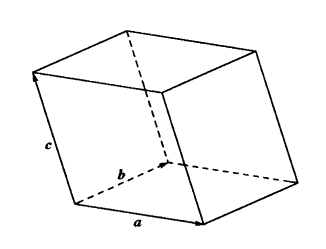
\includegraphics[width=5cm]{/media/wu/file/stuuudy/notes/images/miscellaneous/Parallelepiped.png}
\end{center}

用如下三阶方阵表示
\begin{equation*}
A=
\begin{bmatrix}
a_1&a_2&a_3\\b_1&b_2&b_3\\
c_1&c_2&c_3
\end{bmatrix}
\end{equation*}
那么,\(\ba,\bb,\bv\)三向量的混合积
\begin{equation*}
V=\ba\cdot(\bb\times\bc)
\end{equation*}
表示这个平行六面体的有向体积,其绝对值等于该平行六面体的体积,当
\(\ba,\bb,\bc\)组成右手系时取正号,反之取负号,记为
\begin{equation*}
V=\abs{A}=
\begin{vmatrix}
a_1&a_2&a_3\\b_1&b_2&b_3\\
c_1&c_2&c_3
\end{vmatrix}
\end{equation*}

按照前面点乘、叉乘的坐标计算公式,有
\begin{align*}
V&=\abs{A}=
\begin{vmatrix}
a_1&a_2&a_3\\
b_1&b_2&b_3\\
c_1&c_2&c_3
\end{vmatrix}\\
&=a_1
\begin{vmatrix}
b_2&b_3\\c_2&c_3\\
\end{vmatrix}-a_2
\begin{vmatrix}
b_1&b_3\\c_1&c_3\\
\end{vmatrix}+a_3
\begin{vmatrix}
b_1&b_2\\c_1&c_2
\end{vmatrix}
\end{align*}
我们把\(\abs{A}\)称为三阶方阵\(A\)的行列式

行列式有如下基本性质
\begin{enumerate}
\item 如果\(\ba,\bb,\bc\)中有一个向量为两个向量的线性组合,例如
\(\ba=k_1\ba_1+k_2\ba_2\),此时
\begin{align*}
\abs{A}&=(k_1\ba_1+k_2\ba_2)\cdot(\bb\times\bc)\\
&=k_1\ba_1\cdot(\bb\times\bc)+k_2\ba_2\cdot(\bb\times\bc)\\
&=k_1\abs{A_1}+k_2\abs{A_2}
\end{align*}
其中\(A_1,A_2\)为分别以\(\ba_1,\ba_2\)为第一行的三阶方阵,这个性质称为 \textbf{行线性}
\item 如果\(\ba,\bb,\bc\)线性相关,即\(A\)的行向量线性相关,不满秩,此时三向量共
勉,平行六面体体积为 0
\end{enumerate}
\subsection{\(n\)阶方阵的行列式}
\label{sec:orgee63107}
设\(A\)是数域\(K\)上的一个\(n\)阶方阵,其行向量组为
\(\alpha_1,\dots,\alpha_n\),列向量组为\(\beta_1,\dots,\beta_n\)


\begin{definition}[]
设\(f\)是定义在\(M_n(K)\)上的数量函数,满足如下条件:对\(K^n\)中任意向量
\(\alpha_1,\dots,\alpha_n,\alpha\)以及\(K\)中任意数 \(\lambda\) 都有
\begin{gather*}
f
\begin{bmatrix}
\alpha_1\\\vdots\\\alpha_i+\alpha\\\vdots\\\alpha_n
\end{bmatrix}=
f
\begin{bmatrix}
\alpha_1\\\vdots\\\alpha_i\\\vdots\\\alpha_n\\
\end{bmatrix}+
f
\begin{bmatrix}
\alpha_1\\\vdots\\\alpha\\\vdots\\\alpha_n
\end{bmatrix}\\
f
\begin{bmatrix}
\alpha_1\\\vdots\\\lambda\alpha_i\\\vdots\\\alpha_n
\end{bmatrix}=f
\begin{bmatrix}
\alpha_1\\\vdots\\\alpha_i\\\vdots\\\alpha_n
\end{bmatrix}
\end{gather*}
则称\(f\)为\(M_n(K)\)上的一个 \textbf{行线性函数}

设\(g\)是定义在\(M_n(K)\)上的一个数量函数,满足:对\(K^n\)中任意向量
\(\beta_1,\dots,\beta_n,\beta\)以及\(K\)中任意数 \(\lambda\) ,都有
\begin{align*}
g(\beta_1,&\cdots,\beta_j+\beta,\cdots,\beta_n)=\\
&=g(\beta_1,\cdots,\beta_j,\cdots,\beta_n)+g(\beta_1,\cdots,\beta,\cdots,\beta_n)\\
g(\beta_1,&\cdots,\lambda\beta_j,\cdots,\beta_n)=\lambda g(\beta_1,\cdots,\beta_j,\cdots,\beta_n)
\end{align*}
则称\(g\)为\(M_n(K)\)上一个 \textbf{列线性函数}
\end{definition}

如果\(M_n(K)\)上一个列线性函数\(f\)满足:当\(A\in M_n(K)\)有两列元素相同时
\(n\ge2\),必有\(f(A)=0\),则\(f\)称为 \textbf{反对称} 的列线性函数

\begin{proposition}[]
设\(f\)是\(M_n(K)(n\ge2)\) 上的反对称列(行)线型函数,则
\begin{enumerate}
\item 设将\(A\in M_n(K)\)的\(i,j\)两列(行)互换得出方阵\(B\),则\(f(B)=-f(A)\)
\item 设将\(A\in M_n(K)\)的第\(j\)列(行)加上其第\(i\)列(行)的 \(\lambda\) 倍得出方阵
\(B\),则有 \(f(B)=f(A)\)
\end{enumerate}
\end{proposition}
\begin{proof}
\begin{enumerate}
\item 设\(A=(\cdots,\beta_i,\cdots,\beta_j,\cdots)\)
\begin{align*}
0&=f(\cdots,\beta_i+\beta_j,\cdots,\beta_i+\beta_j,\cdots)\\
&=f(\cdots,\beta_i,\cdots,\beta_j)+f(\cdots,\beta_j,\cdots,\beta_i,\cdots)
\end{align*}
于是
\begin{equation*}
f(A)=-f(B)
\end{equation*}
\end{enumerate}
\end{proof}

\begin{corollary}[]
设\(f,g\)是\(M_n(K)\)上两个反对称列线性函数,且对某个\(A\in M_n(K)\)有
\(f(A)=g(A)\),设\(A\)经有限次初等列变换变为方阵\(B\),则仍有\(f(B)=g(B)\)
\end{corollary}

\begin{corollary}[]
设\(f\)是\(M_n(K)(n\ge2)\)上的列(行)线型函数,则\(f\)为反对称的充分必要条件
是对\(K\)上任何不满秩\(n\)阶方阵\(A\)都有\(f(A)=0\)
\end{corollary}

\begin{definition}[]
设\(f\)是\(M_n(K)\)上一个列线型函数且满足如下条件
\begin{enumerate}
\item 如果\(A\in M_n(K)\)不满秩,则\(f(A)=0\)
\item 对\(M_n(K)\)内单位矩阵\(E\),有\(f(E)=1\)
\end{enumerate}


则称\(f\)为\(M_n(K)\)上一个 \textbf{行列式函数}
\end{definition}

\begin{proposition}[]
\(M_n(K)\)上的行列式函数是唯一的
\end{proposition}

\begin{proof}
设\(f\)与\(g\)是\(M_n(K)\)上两个行列式函数
\begin{enumerate}
\item 如果\(r(A)<n\),则\(f(A)=g(A)=0\)
\item 如果\(r(A)=n\),则\(A\)可表为\(n\)阶初等矩阵\(P_1,\dots,P_m\)的乘积
\begin{equation*}
A=P_1\dots P_m=EP_1\dots P_m
\end{equation*}
因为\(f,g\)均为\(M_n(K)\)上反对称列线型函数,由\(f(E)=g(E)=1\)推出
\begin{equation*}
f(A)=g(A)
\end{equation*}
\end{enumerate}
\end{proof}

\begin{proposition}[]
设\(f(A)\)是\(M_n(K)\)上的行列式函数,则对一切\(A\in M_n(K)\)有\(f(A')=f(A)\)
\end{proposition}

\begin{proof}
设\(n\ge2\)

若\(r(A)<n\),则\(f(A)=0\)

若\(r(A)=n\),则
\begin{equation*}
A=EP_1\dots P_m
\end{equation*}
令\(B_i=EP_1\dots P_i\),设\(B_0=E\),则\(B_i=B_{i-1}P_i\),
\(f(B_i)=f(B_{i-1}P_i)=\epsilon_i f(B_{i-1})\),其中
\begin{equation*}
\epsilon_i=
\begin{cases}
-1&P_i=P_n(k,l)\\
\lambda&P_i=P_n(\lambda\cdot k)\\
1&P_i=P_n(\lambda\cdot k,l)
\end{cases}
\end{equation*}
设\(P_1,\dots,P_m\)中有\(r\)个第一类初等矩阵,\(s\)个第二类初等矩阵,则
\begin{equation*}
f(A)=\epsilon_1\dots\epsilon_m=(-1)^r\lambda_1\dots\lambda_s
\end{equation*}
因为
\begin{equation*}
A'=EP_m'\dots P_1'
\end{equation*}
如果\(P\)是第一类或第二类初等矩阵,则\(P'=P\),而当\(P\)是第三类初等矩阵时,
\(P'\)也是第三类初等矩阵,因此
\begin{equation*}
f(A')=(-1)^r\lambda_1\dots\lambda_s=f(A)
\end{equation*}
\end{proof}

\begin{proposition}[]
设\(f(A)\)是\(M_n(K)(n\ge2)\)上的行列式函数,则\(f(A)\)是反对称的行线性函数
\end{proposition}


给定\(n\)个互补相同的自然数,把它们按一定次序排列起来:
\begin{equation*}
i_1\; i_2\;\dots i_n
\end{equation*}
称为\(n\)个自然数的一个排列。在上述排列中,如果有一个较大的自然数排在较小的 h
自然素前面,则称为一个 \textbf{反序}

一个排列中包含的反序的总数称为该排列的 \textbf{反序数} 。排列\(i_1\dots i_n\)的反序数
记做\(N(i_1\dots i_n)\)。一个排列的反序数是奇数时,该排列称为 \textbf{奇排列} ,反之称
为 \textbf{偶排列}

给定\(n\)个正整数,按大小顺序排列
\begin{equation*}
1\le i_1<i_2<\dots<i_n
\end{equation*}
现在把它们按任意次序重排,得到\(n\)元排列
\begin{equation*}
j_1\;j_2\dots j_n
\end{equation*}
这个排列的反序数\(N(j_1\dots j_n)\)可用下法计算:先找出排在\(i_1\)前面的数字
有多少个,它们的个数记为\(\tau(i_1)\),然后划去\(i_1\),再看\(i_2\)前面未划的数
字有多少个,其个数记为\(\tau(i_2)\),再划去\(i_2\)\ldots{}.,\(n\)次后,即得
\begin{equation*}
N(j_1\dots j_n)=\tau(i_1)+\dots+\tau(i_n)
\end{equation*}

\begin{proposition}[]
对\(n\)个正整数\(i_1,\dots,i_n\)的一个排列\(j_1\dots j_n\)互换此排列中两个数
\(j_k,j_l\)的位置,则有
\begin{equation*}
(-1)^{N(\cdots j_k\cdots j_l\cdots)}=-(-1)^{N(\cdots j_l\cdots j_k\cdots)}
\end{equation*}
\end{proposition}

\begin{proof}
首先设\(j_k\)与\(j_l\)相邻,即\(l=k+1\),则
\begin{align*}
&N(\cdots j_kj_{k+1}\cdots)+1=N(\cdots j_{k+1}j_k\cdots)\quad(j_k<j_{k+1})\\
&N(\cdots j_kj_{k+1}\cdots)-1=N(\cdots j_{k+1}j_k\cdots)\quad(j_k>j_{k+1})
\end{align*}

现设\(l=k+t(t>1)\),把\(j_k\)与\(j_{k+1},\dots,j_{k+t}\)逐个作相邻元素对换
\(t\)次,每对换一次改变一次负号,共改变\(t\)次负号,最后得
\begin{equation*}
\cdots\hat{j_k}j_{k+1}\cdots j_{k+1-1}j_{k+t}j_k\cdots
\end{equation*}
(\(\hat{j_k}\)表示去掉\(j_k\)),再把\(j_{k+t}\)与前面的
\(j_{k+t-1},\dots,j_{k+1}\)逐次对换\(t-1\)次
\end{proof}

\begin{definition}[]
给定数域\(K\)上的\(n\)阶方阵
\begin{equation*}
A=
\begin{bmatrix}
a_{11}&\dots&a_{1n}\\
\vdots&\ddots&\vdots\\
a_{n1}&\dots&a_{nn}\\
\end{bmatrix}
\end{equation*}
令
\begin{equation*}
\det(A)=\sum_{(j_1\cdots j_n)}(-1)^{N(j_1\cdots j_n)}a_{j_11}\cdots a_{j_nn}
\end{equation*}
其中和号表示对前\(n\)个自然数\(1,2\dots,n\)的所有可能排列\(j_1j_2\cdots j_n\)
求和
\end{definition}

\(\det(A)\)是\(M_n(K)\)上一个数量函数,今后用以下记号表示
\begin{equation*}
\det(A)=\abs{A}=
\begin{vmatrix}
a_{11}&a_{12}&\cdots&a_{1n}\\
a_{21}&a_{22}&\cdots&a_{2n}\\
\vdots&\vdots&\ddots&\vdots\\
a_{n1}&a_{n2}&\cdots&a_{nn}
\end{vmatrix}
\end{equation*}
称为\(A\)的 \textbf{行列式}

\begin{theorem}[]
\(\det(A)\)是\(M_n(K)\)上唯一的行列式函数
\end{theorem}

\begin{proof}
设\(n\ge2\)
\begin{enumerate}
\item 证\(\det(A)\)为列线型函数。设\(A\)第\(k\)列为两向量线性组合
\begin{align*}
A&=(\alpha_1,\dots,\lambda\alpha+\mu\beta,\dots,\alpha_n)\\
A_1&=(\alpha_1,\dots,\alpha,\dots,\alpha_n)\\
A_2&=(\alpha_1,\dots,\beta,\dots,\alpha_n)
\end{align*}
那么
\begin{align*}
\det(A)&=\sum(-1)^{N(i_1\dots i_n)}a_{i_11}\dots a_{i_kk}\dots a_{i_nn}\\
&=\sum(-1)^{N(i_1\dots i_n)}a_{i_11}\dots(\lambda a_{i_k}+\mu b_{i_k})\\
&=\lambda\det(A_1)+\mu\det(A_2)
\end{align*}
\item 证\(\det(A)\)反对称。设\(A\)的\(k,l\)两列向量相同
\begin{equation*}
\begin{bmatrix}
a_{1k}\\a_{2k}\\\vdots\\a_{nk}
\end{bmatrix}=
\begin{bmatrix}
a_{1l}\\a_{2l}\\\vdots\\a_{nl}
\end{bmatrix}=
\begin{bmatrix}
a_1\\a_2\\\vdots\\a_n
\end{bmatrix}
\end{equation*}
考查
\begin{align*}
(-1&)^{N(i_1\cdots i_k\cdots i_l\cdots i_n)}a_{i_11}\cdots a_{i_kk}\cdots a_{i_ll}\cdots
a_{i_nn}\\
&=(-1)^{N(i_1\cdots i_k\cdots i_l\cdots i_n)}a_{i_11}\cdots a_{i_k}\cdots a_{i_l}\cdots
a_{i_nn}\\
(-1&)^{N(i_1\cdots i_l\cdots i_k\cdots i_n)}a_{i_11}\cdots a_{i_lk}\cdots a_{i_kl}\cdots a_{i_nn}\\
&=(-1)^{N(i_1\cdots i_l\cdots i_k\cdots i_n)}a_{i_11}\cdots a_{i_l}
\cdots a_{i_k}\cdots a_{i_nn}
\end{align*}
上面两项相加为 0,因此
\begin{equation*}
\det(A)=0
\end{equation*}
\item 若\(A=E\),则\(\det(A)=1\)
\end{enumerate}
\end{proof}

\begin{corollary}[]
设\(A=(a_{ij})\)为数域\(K\)上的\(n\)阶方阵,则
\begin{equation*}
\abs{A}=\sum_{(i_1\dots i_n)}(-1)^{N(i_1\dots i_n)}a_{1i_1}\dots a_{ni_n}
\end{equation*}
\end{corollary}

\begin{proof}
设\(A'=(a_{ij}')\),则\(a_{ij}'=a_{ji}\),有
\begin{align*}
\abs{A}&=\abs{A'}=\sum_{(i_1\dots i_n)}(-1)^{N(i_1\dots i_)}a_{i_11}'\dots a_{i_nn}'\\
&=\sum_{(i_1\dots i_n)}(-1)^{N(i_1\dots i_n)}a_{1i_1}\dots a_{ni_n}
\end{align*}
\end{proof}

对数域\(K\)上\(n\)阶方阵\(A=(a_{ij})\)去掉\(A\)的第\(i\)行第\(j\)列得到的
\(n-1\)阶方阵记做\(A\binom{i}{j}\),我们有
\begin{equation*}
A\binom{1}{k}=
\begin{bmatrix}
a_{21}&\cdots&a_{2\;k-1}&a_{2\;k+1}&\cdots a_{2n}\\
\vdots&&\vdots&\vdots&&\vdots\\
a_{n1}&\cdots&a_{n\; k-1}&a_{n\;k+1}&\cdots&a_{nn}
\end{bmatrix}
\end{equation*}

\begin{theorem}[]
对数域\(K\)上的\(n\)阶方阵\(A=(a_{ij})\),我们有
\begin{equation*}
\det(A)=\abs{A}=
\sum_{k=1}^n(-1)^{1+k}a_{1+k}\det(A\binom{1}{k})
\end{equation*}
\end{theorem}

\begin{proof}
设\(\epsilon_i=(0,\dot,0,1,0,\dots,0)\)是\(K\)上\(n\)维向量空间\(K^n\)的坐标
向量,设\(A\)的行向量组\(\alpha_1,\dots,\alpha_n\),则
\begin{equation*}
A=
\begin{bmatrix}
\alpha_1\\\alpha_2\\\vdots\\\alpha_n
\end{bmatrix}=
\begin{bmatrix}
\sum_{k=1}^na_{1k}\epsilon_k\\\alpha_2\\\vdots\\\alpha_n
\end{bmatrix}
\end{equation*}
\(\det\)是行线性函数,故
\begin{equation*}
\det(A)=\sum_{k=1}^na_{1k}\det
\begin{bmatrix}
\epsilon_k\\\alpha_2\\\vdots\\\alpha_n
\end{bmatrix}=
\sum_{k=1}^na_{1k}\left(
\sum_{(j_2\dots j_n)}(-1)^{N(kj_2\dots j_n)}a_{2j_2}\dots a_{nj_n}
\right)
\end{equation*}
显然有
\begin{equation*}
N(kj_2\dots j_n)=k-1+N(j_2\dots j_n)
\end{equation*}
因为\(j_2,\dots,j_n\)中恰有\(k-1\)个数小于\(k\),因此
\begin{equation*}
\det
\begin{bmatrix}
\epsilon_k\\\alpha_2\\\vdots\\\alpha_n
\end{bmatrix}=(-1)^{k+1}\det(A\binom{1}{k})
\end{equation*}
\end{proof}

\begin{proposition}[]
我们有
\begin{equation*}
\begin{vmatrix}
a_{11}&&&\bigzero\\
a_{21}&a_{22}&&\\
\vdots&\vdots&\ddots&\\
a_{n1}&a_{n2}&\cdots&a_{nn}
\end{vmatrix}=
a_{11}\dots a_{nn}
\end{equation*}
\end{proposition}
\subsubsection{行列式的性质}
\label{sec:org8061bb0}
\begin{proposition}[]
行列互换,行列式的值不变,\(\abs{A}=\abs{A'}\)
\end{proposition}

\begin{proposition}[]
两行(列)互换,行列式值变号
\end{proposition}

\begin{proposition}[]
若行列式中某行(列)每个元素分为两个数的和,则该行列式可关于该行(列)拆成两
个行列式之和
\end{proposition}

\begin{proposition}[]
行列式中某行(列)有公因子\(\lambda\in K\)时, \(\lambda\) 可提出行列式外
\end{proposition}

\begin{proposition}[]
把行列式的第\(j\)行加上第\(i\)行的\(k\)倍后,其值不变
\end{proposition}

\begin{proposition}[]
一个\(n\)阶方阵\(A\)不满秩,其行列式为 0
\end{proposition}
\subsubsection{行列式对任意行(列)的展开公式}
\label{sec:orga9c9b1c}
行列式\(\abs{A\binom{i}{j}}\)称为\(A\)中元素\(a_{ij}\)的 \textbf{余子式} ,简写成\(M_{ij}\)
\begin{equation*}
\abs{A}=\sum_{k=1}^n(-1)^{k+1}a_{1k}M_{1k}
\end{equation*}
也称为\(n\)阶行列式\(\abs{A}\)对其 \textbf{第一行的展开公式}

\begin{definition}[]
设\(A=(a_{ij})\)为一数域\(K\)上的\(n\)阶公式,
\begin{equation*}
A_{ij}=(-1)^{i+j}M_{ij}=(-1)^{i+j}\abs{A\binom{i}{j}}
\end{equation*}
称为元素\(a_{ij}\)的 \textbf{代数余子式}
\end{definition}

\begin{proposition}[]
\(n\)阶行列式\(\abs{A}\)可按任意一行和任意一列展开,展开公式为
\begin{align*}
&\abs{A}=a_{i1}A_{i1}+\dots+a_{in}A_{in}\\
&\abs{A}=a_{1j}A_{1j}+\dots+A_{nj}A_{nj}
\end{align*}
\end{proposition}

\begin{proposition}[]
\label{prop2.6}
证明范德蒙徳(Vandermonde)行列式
\begin{equation*}
\abs{A}=
\begin{vmatrix}
1&1&\cdots&1\\
a_1&a_2&\cdots&a_n\\
a_1^2&a_2^2&\cdots&a_n^2\\
\vdots&\vdots&&\vdots\\
a_1^{n-1}&a_2^{n-2}&\cdots&a_{n}^{n-1}
\end{vmatrix}=
\prod_{1\le j<i\le n}(a_i-a_j)
\end{equation*}
\end{proposition}

\begin{proof}
\begin{align*}
\prod_{1\le j<i\le n}(a_i-a_j)&=(a_2-a_1)(a_3-a_1)\dots(a_n-a_1)\\
&\times (a_3-a_2)(a_4-a_2)\dots(a_n-a_2)\\
&\times(a_4-a_3)\dots(a_n-a_3)\\
&\times\dots\\
&\times(a_n-a_{n-1})
\end{align*}
数学归纳法,在\(\abs{A}\)中将第\(n\)行减去\(n-1\)行的\(a_1\)倍
\begin{align*}
\abs{A}&=
\begin{vmatrix}
1&1&1&\cdots&1\\
0&a_2-a_1&a_3-a_1&\cdots&a_n-a_1\\
\vdots&\vdots&\vdots&&\vdots\\
0&a_2^{n-1}-a_1a_2^{n-2}&a_3^{n-1}-a_1a_3^{n-2}&\cdots&
a_n^{n-1}-a_1a_n^{n-2}
\end{vmatrix}\\
&=
\begin{vmatrix}
a_2-a_1&a_3-a_1&\cdots&a_n-a_1\\
\vdots&\vdots&&\vdots\\
a_2^{n-1}-a_1a_2^{n-2}&a_3^{n-1}-a_1a_3^{n-2}&\cdots&
a_n^{n-1}-a_1a_n^{n-2}
\end{vmatrix}\\
&=(a_2-a_1)(a_3-a_1)\dots(a_n-a_1)
\begin{vmatrix}
1&1&\cdots&1\\
a_2&a_3&\cdots&a_n\\
\vdots&\vdots&&\vdots\\
a_2^{n-2}&a_3^{n-2}&\cdots&a_n^{n-2}
\end{vmatrix}
\end{align*}
\end{proof}
\subsubsection{行列式的其他重要性质}
\label{sec:org06d518c}
\begin{proposition}[]
给定数域\(K\)上分块\(n\)阶方阵
\begin{equation*}
M=
\begin{bmatrix}
A&C\\0&B
\end{bmatrix}
\end{equation*}
其中\(A\)为\(k\)阶方阵,则\(\abs{M}=\abs{A}\cdot\abs{B}\)
\end{proposition}

\begin{proposition}[]
给定实数域上的\(n\)阶方阵
\begin{equation*}
A(t)=
\begin{bmatrix}
a_{11}(t)&\cdots&a_{1n}(t)\\
\vdots&\vdots&&\vdots\\
a_{n1}(t)&a_{n2}(t)&\cdots&a_{nn}(t)
\end{bmatrix}
\end{equation*}
其中\(a_{ij}(t)\)为开区间\((a,b)\)内的可微函数,则\(\abs{A(t)}\)也是
\((a,b)\)内的可微函数,且
\begin{equation*}
\frac{d}{dt}\abs{A(t)}=\sum_{i=1}^n\abs{A_i(t)}
\end{equation*}
\end{proposition}
\subsection{行列式的初步应用}
\label{sec:orga6f6cb6}
\subsubsection{齐次线性方程组}
\label{sec:orgc6e522d}
\begin{proposition}[]
设\(A_0\)是数域\(K\)上的一个\(n\)阶方阵,则\(A_0\)满秩的充要条件是其行列式\(\abs{A_0}\neq0\)
\end{proposition}

\begin{theorem}[]
数域\(K\)上的\(n\)个未知量\(n\)个方程的齐次线性方程组有非零解的充分必要条件
是其系数矩阵的行列式为零
\end{theorem}
\subsubsection{逆矩阵}
\label{sec:orgd6bd73a}
\begin{equation*}
\delta_{ij}=
\begin{cases}
1&i=j\\
0&i\neq j
\end{cases}
\end{equation*}
称为 \textbf{克朗捏克(Kronecker)记号}
\begin{proposition}[]
\label{prop3.2}
\(n\)阶方阵\(A=(a_{ij})\)的行列式\(\abs{A}\)和它的代数余子式有如下关系
\begin{equation*}
\begin{array}{c}
a_{i1}A_{j1}+\dots+a_{in}A_{jn}=\delta_{ij}\abs{A}\\
a_{1i}A_{1j}+\dots+a_{ni}A_{nj}=\delta_{ij}\abs{A}\\
\end{array}
(i,j=1,2,\dots,n)
\end{equation*}
\end{proposition}
\begin{proof}
把\(A\)的第\(j\)行元素换成\(a_{i1},a_{i2},\dots,a_{in}\),得到矩阵
\(\bbar{A}\),矩阵的\(i,j\)两行相同,故\(\abs{\bbar{A}}=0\),把
\(\abs{\bbar{A}}\)对第\(j\)行展开
\end{proof}

给定数域\(K\)上一个\(n\)阶方阵\(n\ge2\)
\begin{equation*}
A=
\begin{bmatrix}
a_{11}&\dots&a_{1n}\\
\vdots&\ddots&\vdots\\
a_{m1}&\dots&a_{mn}\\
\end{bmatrix}
\end{equation*}
用\(\abs{A}\)的代数余子式排成如下一个\(n\)阶方阵
\begin{equation*}
A^*=
\begin{bmatrix}
A_{11}&\cdots&A_{n1}\\
\vdots&&\vdots\\
A_{1n}&\cdots&A_{nn}
\end{bmatrix}
\end{equation*}

\(A^*\)称为\(A\)的 \textbf{伴随矩阵} 。根据命题 \ref{prop3.2} 有
\begin{align*}
AA^*&=\left(\sum_{k=1}^na_{ik}A_{jk}
\right)=(\delta_{ij}\abs{A})=\abs{A}\cdot E\\
A^*A&=\left(\sum_{k=1}^nA_{ki}a_{kj}
\right)=(\delta_{ij}\abs{A})=\abs{A}\cdot E
\end{align*}
如果\(\abs{A}\neq0\),则有
\begin{equation*}
A^{-1}=\frac{1}{\abs{A}}A^*
\end{equation*}

\begin{theorem}[]
\(n\)阶方阵\(A\)可逆的充分必要条件是\(\abs{A}\neq0\)。在\(A\)可逆且\(n\ge2\)
时有
\begin{equation*}
A^{-1}=\frac{1}{\abs{A}}A^*
\end{equation*}
\end{theorem}

现在考虑\(n\)个未知量\(n\)个方程的线性方程组
\begin{equation*}
\begin{cases}
a_{11}x_1+\dots+a_{1n}x_n=b_1\\
a_{21}x_1+\dots+a_{2n}x_n=b_2\\
\dots\\
a_{n1}x_1+\dots+a_{nn}x_n=b_n
\end{cases}
\end{equation*}
令
\begin{equation*}
A=
\begin{bmatrix}
a_{11}&\dots&a_{1n}\\
\vdots&\ddots&\vdots\\
a_{m1}&\dots&a_{mn}\\
\end{bmatrix},
X=
\begin{bmatrix}
x_1\\\vdots\\x_n
\end{bmatrix},
B=
\begin{bmatrix}
b_1\\\vdots\\b_n
\end{bmatrix}
\end{equation*}
则方程组可写为
\begin{equation*}
AX=B
\end{equation*}
有如下结论
\begin{enumerate}
\item 方程组有唯一解的充分必要条件是\(\abs{A}\neq0\)
\item 当\(\abs{A}\neq0\)时,方程组有唯一解
\begin{equation*}
X=A^{-1}B
\end{equation*}
\end{enumerate}


\begin{align*}
X&=A^{-1}B=\frac{1}{\abs{A}}A^*B\\
&=
\frac{1}{\abs{A}}
\begin{bmatrix}
A_{11}&\dots&A_{n1}\\
\vdots&&\vdots\\
A_{1n}&\dots&A_{nn}
\end{bmatrix}
\begin{bmatrix}
b_1\\\vdots\\b_n
\end{bmatrix}=
\frac{1}{\abs{A}}
\begin{bmatrix}
\sum_{k=1}^nA_{k1}b_k\\\vdots\\
\sum_{k=1}^nA_{kn}b_k
\end{bmatrix}
\end{align*}
令
\begin{equation*}
\abs{A_i}=\sum_{k=1}^nA_{ki}b_k=
\begin{vmatrix}
a_{11}&\dots&a_{1\;i-1}&b_1&a_{1\;i+1}&\dots&a_{1n}\\
\vdots&&\vdots&\vdots&\vdots&&\vdots\\
a_{n1}&\dots&a_{n\;i-1}&b_n&a_{n\;i+1}&\dots&a_{nn}
\end{vmatrix}
\end{equation*}

\(\abs{A_i}\)恰为把\(\abs{A}\)的第\(i\)列换成方程组的常数项而得到的\(n\)阶行
列式,此时方程组的解可表为
\begin{equation*}
X=
\begin{bmatrix}
x_1\\\vdots\\x_n
\end{bmatrix}=
\frac{1}{\abs{A}}
\begin{bmatrix}
\abs{A_1}\\\vdots\\\abs{A_n}
\end{bmatrix}
\end{equation*}
\begin{theorem}[克莱姆(Cramer)法则]
若数域\(K\)上的\(n\)个未知量\(n\)个方程的线性方程组的系数矩阵的行列式
\(\abs{A}\neq0\),则它有唯一解
\begin{equation*}
x_1=\frac{\abs{A_1}}{\abs{A}},\quad\dots,
x_n=\frac{\abs{A_n}}{\abs{A}}
\end{equation*}
其中\(\abs{A_i}\)是把\(\abs{A}\)的第\(i\)列换成方程组的常数项而得到的\(n\)阶
行列式 
\end{theorem}
\subsubsection{矩阵乘积的行列式}
\label{sec:org653c031}
\begin{proposition}[]
设\(P\)是\(n\)阶初等矩阵,\(B\)是任一\(n\)阶方阵,则
\begin{equation*}
\abs{PB}=\abs{P}\cdots\abs{B}
\end{equation*}
\end{proposition}

\begin{proof}
\(PB\)相当于对\(B\)作一次初等行变换
\begin{enumerate}
\item \(P=P_n(i,j),\abs{P}=-1\)
\item \(P=P_n(c\cdot i),\abs{P}=c\)
\item \(P=P_n(k\cdot i,j),\abs{P}=1\)
\end{enumerate}
\end{proof}

\begin{theorem}[]
对数域上任一两个\(n\)阶方阵呢\(A,B\)有
\begin{equation*}
\abs{AB}=\abs{A}\cdot\abs{B}
\end{equation*}
\end{theorem}
\begin{proof}
\begin{enumerate}
\item 若\(\abs{A}=0\),则
\begin{equation*}
r(AB)\le\min\{r(A),r(B)\}<n
\end{equation*}
故\(\abs{AB}=0=\abs{A}\cdot\abs{B}\)
\item 若\(\abs{A}\neq0\),
\begin{equation*}
A=P_1\dots P_s
\end{equation*}
于是
\begin{gather*}
\abs{A}=\abs{P_1}\cdot\dots\cdot\abs{P_s}\\
\abs{AB}=\abs{P_1\dots P_sB}=\abs{P_1}\cdot\dots\cdot\abs{P_s}\cdot\abs{B}=\abs{A}\cdot\abs{B}
\end{gather*}
\end{enumerate}
\end{proof}

\begin{examplle}[]
给定数域\(K\)上的\(n\)阶循环矩阵
\begin{equation*}
A=
\begin{bmatrix}
a_1&a_2&a_3&\dots&a_n\\
a_n&a_1&a_2&\dots&a_{n-1}\\
a_{n-1}&a_n&a_1&\dots&a_{n-2}\\
\vdots&\vdots&\vdots&&\vdots\\
a_2&a_3&a_4&&a_1
\end{bmatrix}
\end{equation*}

令\(epsilon_k=e^{\frac{2k\pi i}{n}}\)为 1 的\(n\)个\(n\)次根,\(x^n=1\),构造\(\C\)上
\(n\)阶方阵
\begin{equation*}
B=
\begin{bmatrix}
1&1&\dots&1\\
\epsilon_1&\epsilon_2&\dots&\epsilon_n\\
\vdots&\vdots&&\vdots\\
\epsilon_1^{n-1}&\epsilon_2^{n-1}&&
\epsilon_n^{n-1}
\end{bmatrix}
\end{equation*}
由 \ref{prop2.6} 可知\(\abs{B}\neq0\)

令\(f(x)=a_1+a_2x+\dots+a_nx^{n-1}\)为\(K\)上多项式,我们有
\begin{align*}
&f(\epsilon_k)=a_1+a_2\epsilon_k+\dots+a_n\epsilon_k^{n-1}\\
&\epsilon_k f(\epsilon_k)=a_n+a_1\epsilon_k+\dots+a_{n-1}\epsilon_k^{n-1}\\
&\epsilon_k^2 f(\epsilon_k)=a_{n-1}+a_n\epsilon_k+\dots+a_{n-2}\epsilon_k^{n-1}\\
&\dots\\
&\epsilon_k^{n-1}f(\epsilon_k)=a_2+a_3\epsilon_k+\dots+a_1\epsilon_k^{n-1}\\
\end{align*}
于是
\begin{align*}
AB&=
\begin{bmatrix}
a_1&a_2&\dots&a_n\\
a_n&a_1&\dots&a_{n-1}    \\
\vdots&\vdots&&\vdots\\
a_2&a_3&\dots&a_1
\end{bmatrix}
\begin{bmatrix}
1&1&\dots&1\\
\epsilon_1&\epsilon_2&\dots&\epsilon_n\\
\vdots&\vdots&&\vdots\\
\epsilon_1^{n-1}&\epsilon_2^{n-1}&&
\epsilon_n^{n-1}
\end{bmatrix}\\
&=
\begin{bmatrix}
f(\epsilon_1)&f(\epsilon_2)&\dots&f(\epsilon_n)\\
\epsilon_1 f(\epsilon_1)&\epsilon_2 f(\epsilon_2)&\dots&
\epsilon_nf(\epsilon_n)\\
\vdots&\vdots&&\vdots\\
\epsilon_1^{n-1}f(\epsilon_1)&
\epsilon_2^{n-1}f(\epsilon_2)&
\dots&
\epsilon_n^{n-1}f(\epsilon_n)&
\end{bmatrix}
\end{align*}
\begin{equation*}
\abs{A}\cdot\abs{B}=\abs{AB}=f(\epsilon_1)\dots f(\epsilon_n)\abs{B}
\end{equation*}
\end{examplle}
\subsubsection{矩阵的秩域行列式}
\label{sec:org0347605}
给定数域\(K\)上的\(m\times n\)矩阵
\begin{equation*}
A=
\begin{bmatrix}
a_{11}&\dots&a_{1n}\\
\vdots&\ddots&\vdots\\
a_{m1}&\dots&a_{mn}\\
\end{bmatrix}
\end{equation*}
给定\(2r\)个正整数\(i_1,\dots,i_r,j_1,\dots,j_r\),其中可有相同者且
\(i_1,\dots,i_r\in\{1,2,\dots,m\}\),\(j_1,\dots,j_r\in\{1,\dots,n\}\),定义
\begin{equation*}
A\left\{
\begin{array}{cccc}
i_1&i_2&\dots&i_r\\
j_1&j_2&\dots&j_r\\
\end{array}
\right\}=
\begin{vmatrix}
a_{i_1j_1}&a_{i_1j_2}&\dots&a_{i_1j_r}\\
a_{i_2j_1}&a_{i_2j_2}&\dots&a_{i_2j_r}\\
\vdots&\vdots&&\vdots\\
a_{i_rj_1}&a_{i_rj_2}&\dots&a_{i_rj_r}\\
\end{vmatrix}
\end{equation*}
称为\(A\)的一个 \textbf{\(r\)阶子式}

\begin{proposition}[]
数域\(K\)上一个\(m\times n\)矩阵\(A\)的秩为\(m\)的充分必要条件是它有一\(m\)
阶子式不为 0
\end{proposition}

\begin{proof}
设\(r(A)=m\),则\(A\)有\(m\)个列向量\(\alpha_{i_1},\dots,\alpha_{i_m}\)线性
无关,以它们为列向量的\(m\)阶方阵的行列式记为\(A\)的一个\(m\)阶子式

设\(A\)有\(m\)阶子式
\begin{equation*}
A\left\{
\begin{array}{cccc}
i_1&i_2&\dots&i_m\\
j_1&j_2&\dots&j_m
\end{array}
\right\}\neq0
\end{equation*}
则\(i_1,\dots,i_m\)无相同者,故必为\(1,2,\dots,m\)的一个排列,即
\begin{equation*}
A\left\{
\begin{array}{cccc}
i_1&i_2&\dots&i_m\\
j_1&j_2&\dots&j_m
\end{array}
\right\}=\pm
A\left\{
\begin{array}{cccc}
1&2&\dots&m\\
j_1&j_2&\dots&j_m
\end{array}
\right\}\neq0
\end{equation*}
这表明\(A\)的第\(j_1,\dots,j_m\)列向量线性无关
\end{proof}

\begin{proposition}[]
设\(A\)是数域\(K\)上一个\(m\times n\)矩阵,则\(r(A)=r\)的充分必要条件是
\(A\)有一\(r\)阶子式不为\(0\),而所有\(r+1\)阶子式都为 0
\end{proposition}
\section{线性空间与线性变换}
\label{sec:org34bfd91}
\subsection{线性空间的基本概念}
\label{sec:org05d7841}
\begin{definition}[]
设\(V\)是一个非空集合,\(K\)是一个数域,又设
\begin{enumerate}
\item 在\(V\)中定义了 \textbf{加法} 对\(V\)中任意两个元素 \(\alpha\) 与 \(\beta\) 都按某一法则对应于\(V\)
内唯一确定的一个元素,记之为 \(\alpha+\beta\)
\item 在\(K\)中的数与\(V\)的元素间定义了一种运算,称为 \textbf{数乘} ,即对\(V\)中任意元
素 \(\alpha\) 和数域 \(K\) 中任意数\(k\),都按某一法则对应于\(V\)内唯一确定的一个元
素,记之为\(k\alpha\)
\end{enumerate}


如果加法与数乘满足下列八条运算法则,那么称\(V\)是数域\(K\)上的一个 \textbf{线性空间}
\begin{enumerate}
\item \(\forall \alpha,\beta,\gamma\in V,\alpha+(\beta+\gamma)=(\alpha+\beta)+\gamma\)
\item \(\forall \alpha,\beta\in V,\alpha+\beta=\beta+\alpha\)
\item \(\exists0\in V\forall a\in V,\alpha+0=\alpha\),此元素 0 称为\(V\)的 \textbf{零元
素}
\item \(\forall a\in V\exists\beta\in V,\alpha+\beta=0\), \(\beta\) 称为 \(\alpha\) 的一个 \textbf{负元
素}
\item 对数域中的数 1,有\(1\cdot\alpha=\alpha\)
\item \(\forall k,l\in K,\alpha\in V,(kl)\alpha=k(l\alpha)\)
\item \(\forall k,l\in K,\alpha\in V,(k+l)\alpha=k\alpha+l\alpha\)
\item \(\forall k\in K,\alpha,\beta\in V,k(\alpha+\beta)=k\alpha+k\beta\)
\end{enumerate}
\end{definition}

把线性空间的元素称为 \textbf{向量}

性质
\begin{enumerate}
\item \(V\)中零向量唯一
\item \(V\)中任一向量 \(\alpha\) 的负向量唯一
\item 加法有消去律
\item 加法可移项
\item \(0\cdot\alpha=0;(-1)\alpha=-\alpha,k\cdot0=0\)
\item 若\(k\alpha=\beta,k\neq0\),则\(\alpha=\frac{1}{k}\beta\)
\end{enumerate}


\begin{proposition}[]
设\(V\)是数域\(K\)上的一个线性空间,如果在\(V\)中存在\(n\)个线性无关的向量
\begin{equation}
\epsilon_1,\dots,\epsilon_n\label{eq4.1.1}
\end{equation}
使\(V\)中任意向量均能被 \eqref{eq4.1.1} 线性表示,那么有
\begin{enumerate}
\item 任给\(V\)内\(n\)个线性无关向量
\begin{equation}
\eta_1,\dots,\eta_n\label{eq4.1.1.2}
\end{equation}
则\(V\)中任意向量都能被 \eqref{eq4.1.1.2} 线性表示
\item 如果\(\eta_1,\dots,\eta_s\)是\(V\)的一个线性无关组,且\(V\)内任一向量都能
被它们线性表示,则\(s=n\)
\end{enumerate}
\end{proposition}

\begin{proof}
\begin{enumerate}
\item Corollary \ref{col2.1.5.2}
\end{enumerate}
\end{proof}

\begin{definition}[]
设\(V\)是数域\(K\)上的一个线性空间,如果\(V\)中存在\(n\)个线性无关的向量
\begin{equation*}
\epsilon_1,\dots,\epsilon_n
\end{equation*}
使\(V\)中任一向量均能被此向量组线性表示,则\(V\)称为 \textbf{\(n\)维线性空间} ,记做
\(\dim V=n\)。上述向量组称为\(V\)的一组 \textbf{基} 。单由零向量组成的线性空间称为 \textbf{零
空间}
\end{definition}

\begin{corollary}[]
设\(V\)是数域\(K\)上的\(n\)维线性空间\(\alpha_1,\dots,\alpha_n\)是\(V\)中一个
向量组,使\(V\)中任一向量可被它线性表示,则此向量组为\(V\)的一组基
\end{corollary}

设\(V\)是数域\(K\)上的\(n\)维线性空间,而
\begin{equation*}
\epsilon_1,\dots,\epsilon_n
\end{equation*}
是它的一组基。任给\(\alpha\in V\),有表示式
\begin{equation*}
a=a_1\epsilon_1+\dots+a_n\epsilon_n
\end{equation*}
由于\(\epsilon_1,\dots,\epsilon_n\)线性无关,表达式的系数唯一确定,我们称
\(a_1,\dots,a_n\)为 \(\alpha\) 在基\(\epsilon_1,\dots,\epsilon_n\)下的 \textbf{坐标}

\begin{examplle}[]
考虑\(n\)维线性空间\(K[x]_n\),它的一个向量\(f(x)\)为\(x\)的一个一元多项式
\begin{equation*}
f(x)=a_0+a_1x+\dots+a_{n-1}x^{n-1}
\end{equation*}
他在基\(1,x,x^2,\dots,x^{n-1}\)的坐标为\(a_0,\dots,a_{n-1}\)
\begin{equation*}
f(x)=(1,x,\dots,x^{n-1})
\begin{bmatrix}
a_0\\a_1\\\vdots\\a_{n-1}
\end{bmatrix}
\end{equation*}
任给\(a\in K\),按二项展开公式
\begin{equation*}
x^k=(x-a+a)^k=\sum_{i=0}^k\binom{k}{i}a^i(x-a)^{k-i}
\end{equation*}
这表明
\begin{equation*}
1,x-a,\dots,(x-a)^{n-1}
\end{equation*}
与基\(1,\dots,x^{n-1}\)等价,从而它也是一组基
\end{examplle}

对数域\(K\)上任意多项式
\begin{equation*}
f(x)=a_0x^m+\dots+a_{m-1}x+a_m
\end{equation*}
定义
\begin{equation*}
f'(x)=a_0mx^{m-1}+a_1(m-1)x^{m-2}+\dots+a_{m-1}
\end{equation*}
称\(f'(x)\)为\(f(x)\)的 \textbf{形式微商} 。对\(K\)上任意两个多项式\(f(x),g(x)\)及任意
\(k\in K\)
\begin{align*}
&(f(x)+g(x))'=f'(x)+g'(x)\\
&(kf(x))'kf='(x)\\
&(f(x)g(x))'=f'(x)g(x)+f(x)g'(x)
\end{align*}

现在设\(f(x)\)是\(K[x]_n\)内任意多项式,\(a\)为\(K\)内任意数,那么有
\begin{equation*}
f(x)=a_0+a_1(x-a)+a_2(x-a)^2+\dots+a_{n-1}(x-a)^{n-1}
\end{equation*}
对\(f(x)\)逐次求形式微商,再令\(x=a\)代入,得
\begin{align*}
&a_0=f(a)\\
&a_1=f'(a)\\
&a_2=\frac{1}{2!}f''(a)\\
&\dots\\
&a_{n-1}=\frac{1}{(n-1)!}f^{(n-1)}(a)
\end{align*}
于是
\begin{align*}
f(x)=&f(a)+f'(a)(x-a)+\frac{f''(a)}{2!}(x-a)^2\\
&+\dots+\frac{f^{(n-1)}(a)}{(n-1)!}(x-a)^{n-1}
\end{align*}
称为数域\(K\)上多项式的 Taylor 展开式,因此
\begin{equation*}
f(x)=(1,x-a,(x-a)^2,\dots,(x-a)^{n-1})
\begin{bmatrix}
f(a)\\f'(a)\\\vdots\\\frac{f^{(n-1)}(a)}{(n-1)!}
\end{bmatrix}
\end{equation*}

\begin{examplle}[]
\label{example4.1.15}
设在\(K^n\)中给定一组基及及向量 \(\beta\)
\begin{equation*}
\alpha_1=
\begin{bmatrix}
a_{11}\\\vdots\\a_{n1}
\end{bmatrix},
\alpha_2=
\begin{bmatrix}
a_{12}\\\vdots\\a_{n2}
\end{bmatrix},\dots
\alpha_n=
\begin{bmatrix}
a_{1n}\\\vdots\\a_{nn}
\end{bmatrix},
\beta=
\begin{bmatrix}
b_1\\\vdots\\b_n
\end{bmatrix},
\end{equation*}
求
\begin{equation*}
x_1\alpha_1+\dots+x_n\alpha_n=\beta
\end{equation*}
就得到 \(\beta\) 在\(\alpha_1,\dots,\alpha_n\)下的坐标,因为\((\alpha_i)\)满秩,
\begin{equation*}
\bbar{A}=
\begin{bmatrix}
a_{11}&\dots&a_{1n}&b_1\\
\vdots&\ddots&\vdots&\vdots\\
a_{m1}&\dots&a_{mn}&b_n\\
\end{bmatrix}\xrightarrow{\text{line exchange}}
\begin{bmatrix}
&c_1\\
&c_2\\
\Huge E&\vdots\\
&c_n
\end{bmatrix}
\end{equation*}
\((c_i)\)即为坐标
\end{examplle}

\begin{proposition}[]
\label{prop4.1.2}
设\(V\)是数域\(K\)上的\(n\)维线性空间,在\(V\)内取定一组基
\(\epsilon_1,\dots,\epsilon_n\),设\(V\)内向量组\(\alpha_1,\dots,\alpha_s\)中
各向量在此组基下的坐标表示式为
\begin{equation*}
\alpha_i=(\epsilon_1,\dots,\epsilon_n)A_i
\end{equation*}
则\(\alpha_1,\dots,\alpha_s\)线性无关(相关)的充要条件是\(A_1,\dots,A_s\)在
\(K^n\)内线性无关(相关)
\end{proposition}

设在\(n\)维线性空间\(V\)内给定两组基
\begin{align*}
\epsilon_1,\dots,\epsilon_n\\
\eta_1,\dots,\eta_n
\end{align*}
每个\(\eta_i\)都能被\(\epsilon_1,\dots,\epsilon_n\)线性表示,设
\begin{align*}
&\eta_1=t_{11}\epsilon_1+\dots+t_{n1}\epsilon_n\\
&\dots\\
&\eta_n=t_{1n}\epsilon_1+\dots+t_{nn}\epsilon_n
\end{align*}
可写成
\begin{equation*}
(\eta_1,\dots,e_1)=(\epsilon_1,\dots,\epsilon_n)
\begin{bmatrix}
t_{11}&\cdot&t_{1n}\\
\vdots&&\vdots\\
t_{n1}&\dots&t_{nn}
\end{bmatrix}
\end{equation*}
令
\begin{equation*}
T=
\begin{bmatrix}
t_{11}&\dots&t_{1n}\\
\vdots&\ddots&\vdots\\
t_{m1}&\dots&t_{mn}\\
\end{bmatrix}
\end{equation*}
称\(T\)为从基\(\epsilon_1,\dots,\epsilon_n\)到基\(\eta_1,\dots,\eta_n\)的 \textbf{过
渡矩阵}

\begin{proposition}[]
在数域\(K\)上的\(n\)维线性空间\(V\)内给定一组基
\(\epsilon_1,\dots,\epsilon_n\)。\(T\)是\(K\)上一个\(n\)阶方阵,令
\begin{equation*}
(\eta_1,\dots,\eta_n)=(\epsilon_1,\dots,\epsilon_n)T
\end{equation*}
则
\begin{enumerate}
\item 如果\(\eta_1,\dots,\eta_n\)是\(V\)的一组基,则\(T\)可逆
\item 如果\(T\)可逆,则\(\eta_1,\dots,\eta_n\)是\(V\)的一组基
\end{enumerate}
\end{proposition}

\begin{proof}
设\(T\)的列向量组为\(T_1,\dots,T_n\),则\(\eta_1,\dots,\eta_n\)是一组基 iff
线性无关 iff 按命题 \ref{prop4.1.2} \(T_1,\dots,T_n\)线性无关 等价与满秩
\end{proof}

\index{过渡矩阵}
设\(V\)中一个向量 \(\alpha\) 在第一组基\(\epsilon_1,\dots,\epsilon_n\)下的坐标为
\(x_1,\dots,x_n\),在基\(\eta_1,\dots,\eta_n\)下的坐标为\(y_1,\dots,y_n\),设
两组基的过渡矩阵为\(T\),令
\begin{equation*}
X=
\begin{bmatrix}
x_1\\\vdots\\x_n
\end{bmatrix},\quad
Y=
\begin{bmatrix}
y_1\\\vdots\\y_n
\end{bmatrix}
\end{equation*}
则
\begin{equation*}
\alpha=(\epsilon_1,\dots,\epsilon_n)X=(\eta_1,\dots,\eta_n)Y
=(\epsilon_1,\dots,\epsilon_n)TY
\end{equation*}
因此
\begin{equation*}
X=TY
\end{equation*}
\textbf{坐标变换公式}

在\(K^n\)中,设第一组基为
\begin{align*}
&\epsilon_1=(a_{11},\dots,a_{n1})\\
&\dots\\
&\epsilon_n=(a_{1n},\dots,a_{nn})
\end{align*}
第二组基为
\begin{align*}
&\eta_1=(b_{11},\dots,b_{n1})\\
&\dots\\
&\eta_n=(b_{1n},\dots,b_{nn})
\end{align*}
而
\begin{equation*}
(\eta_1,\dots,\eta_n)=(\epsilon_1,\dots,\epsilon_n)T
\end{equation*}
\(T\)的第\(i\)个列向量的分量是\(\eta_i\)在基\(\epsilon_1,\dots,\epsilon_n\)下
的坐标,
令
\begin{equation*}
A=
\begin{bmatrix}
a_{11}&\dots&a_{1n}\\
\vdots&\ddots&\vdots\\
a_{m1}&\dots&a_{mn}\\
\end{bmatrix},\quad
B=
\begin{bmatrix}
b_{11}&\dots&b_{1n}\\
\vdots&\ddots&\vdots\\
b_{m1}&\dots&b_{mn}\\
\end{bmatrix}
\end{equation*}
做
\begin{equation*}
\begin{pmatrix}
A&\vdots&B
\end{pmatrix}\xrightarrow{\text{line exchange}}
\begin{pmatrix}
E&\vdots&T
\end{pmatrix}
\end{equation*}
\subsection{子空间与商空间}
\label{sec:org4a86c2d}

\begin{definition}[]
设\(V\)是数域\(K\)上的一个线性空间,\(M\)是\(V\)的一个非空子集,如果\(M\)关于
\(V\)内的加法与数乘运算也组成数域\(K\)上的一个线性空间,则\(M\)称为\(V\)的一
个 \textbf{子空间}
\end{definition}

\begin{proposition}[]
线性空间\(V\)的一个非空子集\(M\)是一个子空间的充要条件是满足
\begin{enumerate}
\item 对加法封闭
\item 对数乘封闭
\end{enumerate}
\end{proposition}

设\(\alpha_1,\dots,\alpha_s\)是\(V\)内一个向量组
\begin{equation*}
L(\alpha_1,\dots,\alpha_s)=\{k_1\alpha_1+\dots+k_s\alpha_s\mid
k_i\in K\}
\end{equation*}
是 \textbf{由向量组\(\alpha_1,\dots,\alpha_s\)生成的子空间}

对一个线性空间\(V\),单由它的零向量组成的子集也是一个子空间,称作 \textbf{零子空间} ,
记做\(\{0\}\),另外自身也是一个子空间,这两个子空间称为\(V\)的 \textbf{平凡子空间}

\begin{proposition}[]
设\(V\)是数域\(K\)上的\(n\)维线性空间,\(M\)是\(V\)的一个非零子空间,则\(M\)
内任一组基都可以扩充成\(V\)的一组基
\end{proposition}

\begin{corollary}[]
一个有限维线性空间\(V\)内任意\(r\)个线性无关的向量
\(\alpha_1,\dots,\alpha_r\)都可以扩充为\(V\)的一组基
\end{corollary}

\begin{definition}[]
设\(M_1,M_2\)为线性空间\(V\)的两个子空间,称\(M_1\cap M_2\)为它们的交
\begin{equation*}
M=\{\alpha_1+\alpha_2\mid\alpha_1\in M_1,\alpha_2\in M_2\}
\end{equation*}
称为\(M_1\)与\(M_2\)的 \textbf{和} ,记做\(M_1+M_2\)
\end{definition}

\begin{proposition}[]
设\(M_1,M_2\)为线性空间\(V\)的两个子空间,则它们的交\(M_1\cap M_2\)与和
\(M_1+M_2\)仍是\(V\)的子空间
\end{proposition}

\begin{theorem}[维数公式]
设\(M_1,M_2\)是线性空间\(V\)的两个有限维子空间,则有
\begin{equation*}
\dim(M_1+M_2)=\dim M_1+\dim M_2-\dim(M_1\cap M_2)
\end{equation*}
\end{theorem}

\begin{corollary}[]
设\(M_1,\dots,M_k\)是线性空间\(V\)的\(k\)个有限维子空间,则
\begin{equation*}
\dim(M_1+\dots+M_k)\le\dim M_1+\dots+\dim M_k
\end{equation*}
\end{corollary}

\begin{definition}[]
设\(M_1,M_2\)是线性空间\(V\)的两个子空间,\(M_1+M_2=M\),如果对\(M\)内任一向
量 \(\alpha\) ,其表达式
\begin{equation*}
\alpha=\alpha_1+\alpha_2\quad(\alpha_1\in M_1,\alpha_2\in M_2)
\end{equation*}
是唯一的,则称\(M\)是\(M_1\)与\(M_2\)的 \textbf{直和} ,记做
\begin{equation*}
M=M_1\oplus M_2
\end{equation*}
\end{definition}

\begin{theorem}[]
设\(M_1,M_2\)是数域\(K\)上线性空间\(V\)的两个有限维子空间,则下列等价
\begin{enumerate}
\item \(M_1+M_2\)是直和
\item 0 向量表法唯一,即由
\begin{equation*}
0=\alpha_1+\alpha_2(\alpha_1\in M_1,\alpha_2\in M_2)
\end{equation*}
必定有\(\alpha_1=\alpha_2=0\)
\item \(M_1\cap M_2=\{0\}\)
\item \(\dim M_1+\dim M_2=\dim(M_1+M_2)\)
\end{enumerate}
\end{theorem}

\begin{definition}[]
设\(M_1,\dots,M_k\)为线性空间\(V\)的子空间,\(M_1+\dots+M_k=M\)。如果对\(M\)
中任意向量 \(\alpha\) ,表达式
\begin{equation*}
\alpha=\alpha_1+\dots+\alpha_k\quad(\alpha_i\in M_k)
\end{equation*}
是唯一的,则称\(M\)是\(M_1,\dots,M_k\)的 \textbf{直和} ,记做
\begin{equation*}
M=M_1\oplus\dots\oplus M_k=\bigoplus_{i=1}^kM_i
\end{equation*}
\end{definition}

\begin{theorem}[]
设\(M_1,\dots,M_k\)是数域\(K\)上线性空间\(V\)的有限维子空间,则下列命题等价
\begin{enumerate}
\item \(M=M_1+\dots+M_k\)是直和
\item 零向量的表法唯一
\item \(M_i\cap\left(\displaystyle\sum_{\substack{j=1\\j\neq i}}^kM_j\right)=\{0\}\)
\item \(\dim\sum_{i=1}^kM_i=\sum_{i=1}^k\dim M_i\)
\end{enumerate}
\end{theorem}

\begin{corollary}[]
设\(V\)是数域\(K\)上的\(n\)维线性空间,\(M_1,\dots,M_k\)是其子空间,且
\begin{equation*}
V=M_1\oplus\dots\oplus M_k
\end{equation*}
则在每个子空间内取一组基,合并后即成\(V\)的一组基
\end{corollary}

\begin{proposition}[]
设\(M\)是数域\(K\)上有限维线性空间\(V\)的一个子空间,则必存在\(V\)的子空间
\(N\)使
\begin{equation*}
V=M\oplus N
\end{equation*}
\end{proposition}

\begin{definition}[]
设 \(\alpha\) 是\(V\)的一个向量,如果\(V\)的一个向量\(\alpha'\)满足:
\(\alpha'-\alpha\in M\),则称\(\alpha'\)与 \(\alpha\) \textbf{模\(M\)同余} ,记做
\(\alpha'\equiv\alpha(\mod M)\)
\end{definition}

模\(M\)是个等价关系,设\(\alpha\)是\(V\)中任意一个向量,定义
\begin{equation*}
\alpha+M=\{\alpha+m\mid m\in M\}
\end{equation*}
我们称\(\alpha+M\)为一个模\(M\)的 \textbf{同余类} 或称为 \textbf{模\(M\)的剩余类}

性质
\begin{enumerate}
\item \(\alpha'\equiv\alpha(\mod M)\Leftrightarrow\alpha'-\alpha\in
      M\Leftrightarrow\alpha'\in\alpha+M\)
\item \(\alpha'\in\alpha+M\Leftrightarrow\alpha'+M=\alpha+M\)
\item \(a+M=0+M\Leftrightarrow\alpha\in M\)
\item 若\(\alpha'+M\neq\alpha+M\)则\((\alpha'+M)\cap(\alpha+M)=\emptyset\)
\end{enumerate}


令\(\bbar{V}\)表示\(V\)内向量模\(M\)的同余类的全体所成的集合,定义
\begin{enumerate}
\item 加法
\begin{equation*}
(\alpha+M)+(\beta+M)=(\alpha+\beta)+M
\end{equation*}
\item 数乘,对任意\(k\in K\)
\begin{equation*}
k(\alpha+M)=k\alpha+M
\end{equation*}
\end{enumerate}


验证\(\bbar{V}\)确实是线性空间,称为 \textbf{商空间} ,记做\(V/M\)

\begin{proposition}[]
设\(V\)是数域\(K\)上的\(n\)维线性空间,\(M\)是\(V\)的一个\(m\)为子空间,则
\(\dim V/M=n-m\)
\end{proposition}

\begin{proof}
在\(M\)内取一组基\(\epsilon_1,\dots,\epsilon_m\)扩充为\(V\)的一组基
\(\epsilon_1,\dots,\epsilon_n\),证明
\(\bbar{\epsilon}_{m+1},\dots,\bbar{\epsilon}_n\)是\(V/M\)的一组基
\end{proof}
\subsection{线性映射与线性变换}
\label{sec:org09ed561}
\begin{definition}[]
设\(U,V\)为数域\(K\)上的两个线性空间,\(f\)为\(U\)到\(V\)的一个映射,且满足
\begin{enumerate}
\item \(\forall\alpha,\beta\in U\)
\begin{equation*}
f(\alpha+\beta)=f(\alpha)+f(\beta)
\end{equation*}
\item \(\forall a\in U,k\in K\)
\begin{equation*}
f(k\alpha)=kf(\alpha)
\end{equation*}
\end{enumerate}


则称\(f\)为\(U\)到|(V)的一个 \textbf{线性映射} ,\(U\)到\(V\)的全体线性映射所成的集合
记做\(\Hom(U,V)\)
\end{definition}

\begin{proposition}[]
设\(U,V\)是数域\(K\)上的线性空间,\(f\)是\(U\)到\(V\)的线性映射,且为单射,则
\(U\)内向量组\(\alpha_1,\dots,\alpha_l\)线性无关的充要条件是
\(f(\alpha_1),\dots,f(\alpha_l)\)在\(V\)内线性无关
\end{proposition}

\begin{proposition}[]
设\(U,V\)是数域\(K\)上的线性空间,\(\dim U=n\),\(f\)是\(U\)到\(V\)的线性映射,
如果\(f\)是双射,则对\(U\)的任一组基\(\epsilon_1,\dots,\epsilon_n\),
\(f(\epsilon_1),\dots,f(\epsilon_n)\)为\(V\)的一组基,从而\(\dim V=n\)
\end{proposition}

\begin{definition}[]
设\(U,V\)是数域\(K\)上的线性空间,如果存在\(U\)到\(V\)的线性映射\(f\)同时是双
射,则称\(U\)与\(V\) \textbf{同构} ,而\(f\)称为\(U\)到\(V\)的 \textbf{同构映射}
\end{definition}
\begin{proposition}[]
设\(U,V\)是数域\(K\)上的线性空间,\(f\)是\(U\)到\(V\)的同构映射,则\(f^{-1}\)
是\(V\)到\(U\)的同构映射
\end{proposition}

\begin{definition}[]
设\(U,V\)是数域\(K\)上的线性空间,\(f\)是\(U\)到\(V\)的线性映射,定义
\begin{equation*}
\ker f=\{\alpha\in U\mid f(\alpha)=0\}
\end{equation*}
称为线性映射\(f\)的 \textbf{核}
\begin{equation*}
\im f=\{f(\alpha)\mid \alpha\in U\}
\end{equation*}
称为线性映射\(f\)的 \textbf{像集}
\end{definition}

\begin{proposition}[]
设\(U,V\)是数域\(K\)上的线性空间,\(f\in\Hom(U,V)\),则
\begin{enumerate}
\item \(\ker f\)是\(U\)的子空间,\(f\)是单射的充分必要条件是\(\ker f=\{0\}\)
\item \(\im f\)是\(V\)的子空间,定义\(\coker f=V/\im f\)。\(f\)是满射的充分必要
条件是
\begin{equation*}
\coker f=\{0\}
\end{equation*}
\(\coker f\) 称为 \textbf{余核}
\end{enumerate}
\end{proposition}

\begin{proposition}[]
设\(U,V\)是数域\(K\)上的线性空间,\(f\in\Hom(U,V)\),则\(U/\ker f\)与\(\im
   f\)同构
\end{proposition}

\begin{corollary}[]
设\(U,V\)是数域\(K\)上的两个线性空间,\(\dim U=n,f\in\Hom(U,V)\),则
\(\dim\ker f+\dim\im f=\dim U\)
\end{corollary}

\begin{corollary}[]
给定数域\(K\)上\(m\times n\)矩阵\(A\),设\(r(A)=r\),则齐次线性方程组\(AX=0\)
的基础解系含有\(n-r\)个向量
\end{corollary}

\begin{proof}
令\(f_A:K^n\to K^m,X\mapsto AX\),\(\im f_A=L(\alpha_1,\dots,\alpha_n)\),故
\(\dim(\im f_A)=r(A)=r\),有
\begin{equation*}
\dim\ker f_A=\dim K^n-\dim\im f_A=n-r
\end{equation*}
\end{proof}

设\(U,V\)是数域\(K\)上的线性空间
\begin{enumerate}
\item 给定\(f,g\in\Hom(U,V)\),定义
\begin{equation*}
(f+g)\alpha=f(\alpha)+g(\alpha)\quad(\forall\alpha\in U)
\end{equation*}
则\(f+g\in\Hom(U,V)\),称为\(f\)与\(g\)的 \textbf{加法}
\item 给定\(f\in\Hom(U,V),k\in K\),定义
\begin{equation*}
(kf)\alpha=kf(\alpha)\quad(\forall\alpha\in U)
\end{equation*}
则\(kf\in\Hom(U,V)\),称为\(k\)与\(f\)的数乘
\end{enumerate}


零元素为零映射
  \begin{equation*}
0(\alpha)=0
\end{equation*}
因此\(\Hom(U,V)\)关于上述加法、数乘构成\(K\)上的线性空间
\begin{enumerate}
\setcounter{enumi}{2}
\item 设\(U,V,W\)都是数域\(K\)上的线性空间,如果
\(f\in\Hom(U,V),g\in\Hom(V,W)\),定义
\begin{equation*}
(gf)\alpha=g(f(\alpha))
\end{equation*}
显然\(gf\in\Hom(U,W)\),称为\(g\)与\(f\)的 \textbf{乘法}
\end{enumerate}


线性映射的乘法满足
\begin{enumerate}
\item 乘法结合律
\item 加法与乘法分配率
\begin{align*}
&f(g+h)=fg+fh\\
&(f+g)h=fh+gh
\end{align*}
\item 对任意\(k\in K\),\(k(fg)=(kf)g=f(kg)\)
\end{enumerate}


设\(U,V\)是数域\(K\)上的线性空间,且设\(\dim U=n,\dim V=m\),设
\(f\in\Hom(U,V)\),在\(U\)内取定一组基\(\epsilon_1,\dots,\epsilon_n\),在
\(V\)内也取定一组基\(\eta_1,\dots,\eta_n\)

\begin{proposition}[]
\label{prop4.3.6}
\begin{enumerate}
\item \(U\)到\(V\)的任一线性映射\(f\)由它在\(U\)的基\(\epsilon_1,\epsilon_n\)处
的作用唯一决定,即如果有\(g\in\Hom(U,V),g(\epsilon_i)=f(\epsilon_i)\),则
\(f(\alpha)=g(\alpha)(\forall\alpha\in U)\)
\item 任给\(V\)内\(n\)个向量\(\alpha_1,\dots,\alpha_n\),比存在唯一的
\(f\in\Hom(U,V)\)使\(f(\epsilon_i)=\alpha_i(i=1,2,\dots,n)\)
\end{enumerate}
\end{proposition}

根据命题 \ref{prop4.3.6} 只要知道\(f(\epsilon_1),\dots,f(\epsilon_n)\),那么
\(f(\alpha)\)就被唯一决定了,而\(f(\epsilon_i)\)可表为\(V\)的一组基
\(\eta_1,\dots,\eta_n\)的线性组合。设
\begin{align*}
&f(\epsilon_1)=a_{11}\eta_1+\dots+a_{m1}\eta_m\\
&\dots\\
&f(\epsilon_n)=a_{1n}\eta_1+\dots+a_{mn}\eta_m\\
\end{align*}
令
\begin{equation*}
A=
\begin{bmatrix}
a_{11}&\dots&a_{1n}\\
\vdots&\ddots&\vdots\\
a_{m1}&\dots&a_{mn}\\
\end{bmatrix}
\end{equation*}
则
\begin{equation*}
(f(\epsilon_1),\dots,f(\epsilon_n))=(\eta_1,\dots,\eta_n)A
\end{equation*}
\(m\times n\)矩阵\(A\)称为 \textbf{线性映射\(f\)在给定基下的矩阵} 。显然,\(U,V\)的基
取定之后,\(f\)由矩阵\(A\)唯一决定。又有,任给\(K\)上\(m\times n\)矩阵\(A\),
令
\begin{equation*}
(\alpha_1,\dots,\alpha_n)=(\eta_1,\dots,\eta_m)A
\end{equation*}
则存在唯一\(f\in\Hom(U,V)\)使\(f(\epsilon_i)=\alpha_i\),于是\(f\)在所取定基
下的矩阵即为\(A\)

现定义\(\sigma:\Hom(U,V)\to M_{m,n}(K)\)如下:对\(f\in\Hom(U,V)\),如果\(f\)在
\(U,V\)所取定基下的矩阵为 \(A\),则令\(\sigma(f)=A\),由上述讨论, \(\sigma\) 是双射

设\(f\in\Hom(U,V)\),对\(U\)内任一向量组\(\alpha_1,\dots,\alpha_k\),约定
\begin{equation*}
f(\alpha_1,\dots,\alpha_k)=(f(\alpha_1),\dots,f(\alpha_k))
\end{equation*}
令\(\alpha\in U\),则
\begin{align*}
\alpha&=x_1\epsilon_1+\dots+x_n\epsilon_n=(\epsilon_1,\dots,\epsilon_n)X\\
f(\alpha)   &=x_1f(\epsilon_1)+\dots+x_nf(\epsilon_n)\\
&=(f(\epsilon_1),\dots,f(\epsilon_n))X\\
&=[f(\epsilon_1,\dots,\epsilon_n)]X
\end{align*}
一般地,设
\begin{equation*}
\alpha_1=(\epsilon_1,\dots,\epsilon_n)X_1,\dots,\alpha_s=
(\epsilon_1,\dots,\epsilon_n)X_s
\end{equation*}
我们有
\begin{equation*}
f(\alpha_1)=(f(\epsilon_1),\dots,f(\epsilon_n))X_1,\dots,
f(\alpha_s)=(f(\epsilon_1),\dots,f(\epsilon_n))X_s
\end{equation*}
以\(X_1,\dots,X_s\)为列向量排成\(n\times s\)矩阵\(X\),则有
\begin{equation*}
(\alpha_1,\dots,\alpha_s)=(\epsilon_1,\dots,\epsilon_n)X
\end{equation*}
而
\begin{equation*}
(f(\alpha_1),\dots,f(\alpha_s))=(f(\epsilon_1),\dots,f(\epsilon_n))X
\end{equation*}
因此
\begin{equation*}
f[(\epsilon_1,\dots,\epsilon_n)X]=[f(\epsilon_1,\dots,\epsilon_n)]X
\end{equation*}

\begin{proposition}[]
\label{prop4.3.7}
\begin{enumerate}
\item 对\(f,g\in\Hom(U,V),k,l\in K\),有
\begin{equation*}
\sigma(kf+lg)=k\sigma(f)+l\sigma(g)
\end{equation*}
因此 \(\sigma\) 是\(\Hom(U,V)\)到\(M_{m,n}(K)\)的线性空间同构,于是我们有
\begin{equation*}
\dim\Hom(U,V)=\dim M_{m,n}(K)=mn
\end{equation*}
\item 若\(f\in\Hom(U,V),g\in\Hom(V,W)\),则\(\sigma(gf)=\sigma(g)\sigma(f)\)
\end{enumerate}
\end{proposition}


\begin{definition}[]
设\(V\)是数域\(K\)上的线性空间,\(\bA\)是\(V\)到自身的一个线性映射,则称
\(\bA\)为\(V\)内的一个 \textbf{线性变换} 。\(V\)内全体线性变换所成的集合记为\(\End(V)\)
\end{definition}

特殊线性变换
\begin{enumerate}
\item 零变换\(\bzero\)

对任意\(\alpha\in V,\bzero\alpha=0\)

\item 单位变换\(\bE\)

对任意\(\alpha\in V,\bE\alpha=\alpha\)

\item 数乘变换\(\bk\)

对任意\(\alpha\in V,\bk\alpha=k\alpha\)

\item 投影变换

设\(M\)是\(V\)的一个子空间,则存在子空间\(N\)使
\begin{equation*}
V=M\oplus N
\end{equation*}
于是对任意\(\alpha\in V\)有唯一分解式
\begin{equation*}
\alpha=\alpha_1+\alpha_2(\alpha_1\in M,\alpha_2\in N)
\end{equation*}
定义变换如下
\begin{equation*}
\bP\alpha=\alpha_1
\end{equation*}
\end{enumerate}





\begin{proposition}[]
\label{prop4.3.8}
设线性变换\(\bA\)在一组基下的矩阵为\(A\),又设向量 \(\alpha\) 在这组基下的坐标为
\begin{equation*}
X=
\begin{bmatrix}
x_1\\\vdots\\x_n
\end{bmatrix}
\end{equation*}
则\(\bA\alpha\)在这组基下的坐标为\(AX\)
\end{proposition}

\begin{proof}
\begin{align*}
\bA\alpha&=\bA(x_1\epsilon_1+\dots+x_n\epsilon_n)\\
&=\bA[(\epsilon_1,\dots,\epsilon_n)X]\\
&=[\bA(\epsilon_1,\dots,\epsilon_n)]X\\
&=[(\epsilon_1,\dots,\epsilon_n)A]X\\
&=(\epsilon_1,\dots,\epsilon_n)(AX)
\end{align*}
\end{proof}

\begin{proposition}[]
考虑\(K^3\)中一个线性变换\(\bA\),设
\begin{equation*}
\epsilon_1=(1,0,0),\epsilon_2=(0,1,0),\epsilon_3=(0,0,1)
\end{equation*}
则
\begin{equation*}
\bA\epsilon_1=(-1,1,0),\bA\epsilon_2=(2,1,1),\bA\epsilon_3=(0,-1,-1)
\end{equation*}
\begin{enumerate}
\item 求\(\bA\)在基\(\epsilon_1,\epsilon_2,\epsilon_3\)下的矩阵
\item 在\(K^3\)中改取如下一组基
\begin{equation*}
\eta_1=(1,1,1),\eta_2=(1,1,0),\eta_3=(1,0,0)
\end{equation*}
求\(\bA\)在\(\eta_1,\eta_2,\eta_3\)下的矩阵
\end{enumerate}
\end{proposition}

\begin{proof}
\begin{enumerate}
\item 因为
\begin{align*}
&\bA\epsilon_1=-\epsilon_1+\epsilon_2+0\cdot\epsilon_3,\\
&\bA\epsilon_2=2\epsilon_1+\epsilon_2+\epsilon_3,\\
&\bA\epsilon_3=0\cdot\epsilon_1-\epsilon_2-\epsilon_3,\\
\end{align*}
故
\begin{equation*}
(\bA\epsilon_1,\bA\epsilon_2,\bA\epsilon_3)=
(\epsilon_1,\epsilon_2,\epsilon_3)
\begin{bmatrix}
-1&2&0\\1&1&-1\\0&1&-1
\end{bmatrix}
\end{equation*}
\item 因为
\begin{align*}
&\eta_1=\epsilon_1+\epsilon_2+\epsilon_3\\
&\eta_2=\epsilon_1+\epsilon_2\\
&\eta_3=\epsilon_1\\
\end{align*}
故
\begin{align*}
&\bA\eta_1=\bA\epsilon_1+\bA\epsilon_2+\bA\epsilon_3=(1,1,0)\\
&\bA\eta_2=\bA\epsilon_1+\bA\epsilon_2=(1,2,1)\\
&\bA\eta_3=\bA\epsilon_1=(-1,1,0)\\
\end{align*}
由例 \ref{example4.1.15}
\begin{equation*}
\begin{bNiceArray}{ccc:ccc}
1&1&1&1&1&-1\\
1&1&0&1&2&1\\
1&0&0&0&1&0
\end{bNiceArray}\to
\begin{bNiceArray}{ccc:ccc}
1&0&0&0&1&0\\
0&1&0&1&1&1\\
0&0&1&0&-1&-2
\end{bNiceArray}
\end{equation*}
即得
\begin{equation*}
(\bA\eta_1,\bA\eta_2,\bA\eta_3)=(\eta_1,\eta_2,\eta_3)
\begin{bmatrix}
0&1&0\\1&1&1\\0&-1&-2
\end{bmatrix}
\end{equation*}
\end{enumerate}
\end{proof}

\begin{proposition}[]
设
\begin{align*}
\epsilon_1,\dots,\epsilon_n\\
\eta_1,\dots,\eta_n
\end{align*}
是线性空间的两组基,其过渡矩阵是\(T=(t_{ij})\),又设线性变换\(\bA\)在这两组
基下的矩阵分别是\(A\)和\(B\),则
\begin{equation*}
B=T^{-1}AT
\end{equation*}
\end{proposition}

\begin{proof}
由线性变换的矩阵的定义,有
\begin{align*}
&\bA(\epsilon_1,\dots,\epsilon_n)=(\epsilon_1,\dots,\epsilon_n)A\\
&\bA(\eta_1,\dots,\eta_n)=(\eta_1,\dots,\eta_n)B
\end{align*}
则
\begin{equation*}
\bA[(\epsilon_1,\dots,\epsilon_n)T]=[(\epsilon_1,\dots,\epsilon_n)T]B
\end{equation*}
又有
\begin{align*}
\bA[(\epsilon_1,\dots,\epsilon_n)T]&=[\bA(\epsilon_1,\dots,\epsilon_n)]T\\
&=[(\epsilon_1,\dots,\epsilon_n)A]T\\
&=(\epsilon_1,\dots,\epsilon_n)(AT)\\
&=(\epsilon_1,\dots,\epsilon_n)(TB)
\end{align*}
因为\(\epsilon_1,\dots,\epsilon_n\)线性无关,故有
\begin{equation*}
AT=TB
\end{equation*}
而\(T\)可逆
\end{proof}

\begin{definition}[]
对数域\(K\)上的两个\(n\)阶方阵\(A\)与\(B\),如果存在\(K\)上一个\(n\)阶可逆的
方阵\(T\)使\(B=T^{-1}AT\),则称\(B\)与\(A\)在\(K\)内 \textbf{相似} ,记做\(B\sim A\)
\end{definition}

相似是等价关系,我们把数域\(K\)上全体\(n\)阶方阵的集合\(M_n(K)\)在相似关系下
的等价类称作 \textbf{相似类}

\begin{proposition}[]
数域\(K\)上两个\(n\)阶方阵\(A,B\)相似的充分必要条件是它们是\(V\)内某一线性变
换\(\bA\)在两组基下的矩阵
\end{proposition}
\subsection{线性变换的特征值与特征向量}
\label{sec:org5db0f71}
\begin{definition}[]
设\(V\)是数域\(K\)上的一个线性空间,\(\bA\)是\(V\)内一个线性变换,如果对\(K\)
内一个数 \(\lambda\) ,存在\(V\)的一个向量 \(\xi\neq0\),使
\begin{equation*}
\bA\xi=\lambda\xi
\end{equation*}
则称 \(\lambda\) 为\(bA\)的一个 \textbf{特征值} ,而 \(\xi\) 称为属于特征值 \(\lambda\) 的 \textbf{特征向量}
\end{definition}

对于数域\(K\)内任一数 \(\lambda\) ,我们定义
\begin{equation*}
V_\lambda=\{\alpha\in V\mid\bA\alpha=\lambda\alpha\}
\end{equation*}
显然\(0\in V_\lambda\),\(V_\lambda\)关于加法、数乘封闭,即\(V_\lambda\)是
\(V\)的子空间
\begin{enumerate}
\item \(\lambda\in K\)是线性变换\(bA\)的特征值的充分必要条件是
\(V_\lambda\neq\{0\}\).此时\(V_\lambda\)称为\(\bA\)的属于特征值 \(\lambda\) 的 \textbf{特征
子空间}
\item 要找处\(bA\)的属于特征值\(\lambda\)的全部特征向量,只要决定出特征空间
\(V_\lambda\),如果它是有限维子空间只要找它的基
\end{enumerate}


在线性空间和线性变换的问题中,凡是需要具体计算时,就必须在\(V\)内取定一组基
\(\epsilon_1,\dots,\epsilon_n\),求出每个向量在此组基下的坐标
\begin{equation*}
\alpha=x_1\epsilon_1+\dots+x_n\epsilon_n=(\epsilon_1,\dots,\epsilon_n)X
\end{equation*}
再求出线性变换在此组基下的矩阵
\begin{equation*}
(\bA\epsilon_1,\dots,\bA\epsilon_n)=(\epsilon_1,\dots,\epsilon_n)A
\end{equation*}
由命题 \ref{prop4.3.8} ,有
\begin{equation*}
\bA\alpha=(\epsilon_1,\dots,\epsilon_n)(AX)
\end{equation*}
而
\begin{equation*}
\lambda\alpha=(\epsilon_1,\dots,\epsilon_n)(\lambda X)
\end{equation*}
因此\(\bA\alpha=\lambda\alpha\)等价于\(AX=\lambda X\),而\(\alpha\neq0\)等价
于\(X\neq0\)。因\(\lambda X-AX=0\)即\((\lambda E-A)X=0\)
\begin{equation*}
\begin{bmatrix}
\lambda-a_{11}&-a_{12}&\cdots&-a_{1n}\\
-a_{21}&\lambda-a_{22}&\cdots&-a_{2n}\\
\vdots&\vdots&&\vdots\\
-a_{n1}&-a_{n2}&\cdots&\lambda-a_{nn}
\end{bmatrix}
\begin{bmatrix}
x_1\\x_2\\\vdots\\x_n
\end{bmatrix}=0
\end{equation*}
有非零解的成分必要条件是
\begin{equation*}
\abs{\lambda E-A}=0
\end{equation*}

给定数域\(K\)上的\(n\)阶方阵\(A=(a_{ij})\),令
\begin{equation*}
f(\lambda)=\abs{\lambda E-A}=
\begin{vmatrix}
\lambda-a_{11}&-a_{12}&\cdots&-a_{1n}\\
-a_{21}&\lambda-a_{22}&\cdots&-a_{2n}\\
\vdots&\vdots&&\vdots\\
-a_{n1}&-a_{n2}&\cdots&\lambda-a_{nn}
\end{vmatrix}
\end{equation*}
称为方阵\(A\)的 \textbf{特征多项式} ,根称为方阵\(A\)的 \textbf{特征根} 或 \textbf{特征值}


线性变换\(bA\)的特征值和特征向量的计算步骤
\begin{enumerate}
\item 在\(V\)中给定一组基\(\epsilon_1,\dots,\epsilon_n\),求\(\bA\)在这组基下的
矩阵\(A\)
\item 计算特征多项式\(f(\lambda)=\abs{\lambda E-A}\)
\item 求\(f(\lambda)=0\)属于数域\(K\)的那些根
\begin{equation*}
\lambda_1,\dots,\lambda_s
\end{equation*}
\item 对每个\(\lambda_i\),求齐次线性方程组
\begin{equation*}
(\lambda_i E-A)X=0
\end{equation*}
的基础解系
\item 以 4 中求出的基础解系为坐标写出\(V\)中一个向量组,就是\(V_{\lambda_i}\)的一
组基
\end{enumerate}


\begin{examplle}[]
设三维线性空间\(V\)内一个线性变换\(\bA\)在基\(\epsilon_1,\dots,\epsilon_n\)下
的矩阵为
\begin{equation*}
\bA=
\begin{bmatrix}
1&2&2\\2&1&2\\2&2&1
\end{bmatrix}
\end{equation*}
求\(\bA\)的全部特征值和对应的特征向量

\begin{enumerate}
\item 求特征多项式和特征根
\begin{align*}
f(\lambda)&=\abs{\lambda E-A}=
\begin{vmatrix}
\lambda-1&-2&-2\\
-2&\lambda-1&-2\\
-2&-2&\lambda-1
\end{vmatrix}\\
&=\begin{vmatrix}
\lambda-5&-2&-2\\
\lambda-5&\lambda-1&-2\\
\lambda-5&-2&\lambda-1
\end{vmatrix}=(\lambda-5)
\begin{vmatrix}
1&-2&-2\\
1&\lambda-1&-2\\
1&-2&\lambda-1
\end{vmatrix}\\
&=(\lambda-5)
\begin{vmatrix}
1&-2&-2\\
0&\lambda+1&0\\
0&0&\lambda+1
\end{vmatrix}=
(\lambda-5)(\lambda+1)^2
\end{align*}
\(f(\lambda)\)的根为\(\lambda_1=5,\lambda_2=-1\)(二重根)。
\item 求每个特征值对应的特征向量

当\(\lambda_1=5\)时,
\begin{align*}
\lambda_1 E-A&\to
\begin{bmatrix}
1&1&-2\\
0&1&-1\\
0&0&0
\end{bmatrix}\\
&\Leftrightarrow
\begin{cases}
x_1+x_2-2x_3=0\\
x_2-x_3=0
\end{cases}
\end{align*}
令\(x_3=1\)得基础解系\(\eta_1=(1,1,1)\),它对应于\(\bA\)的特征向量
\(\epsilon_1+\epsilon_2+\epsilon_3\),于是他是特征子空间\(V_{\lambda_1}\)
的一组基,即
\begin{equation*}
V_{\lambda_1}=L(\epsilon_1+\epsilon_2+\epsilon_3)
\end{equation*}

当\(\lambda_2=-1\)时
\begin{align*}
\lambda_2 E-A&\to
\begin{bmatrix}
1&1&1\\0&0&0\\0&0&0
\end{bmatrix}\\
&\Leftrightarrow
x_1+x_2+x_3=0
\end{align*}
取\(x_2=1,x_3=0\),得\(\eta_1=(-1,1,0)\),取\(x_2=0,x_3=1\),得
\(\eta_2=(-1,0,1)\),对应于\(\bA\)的一个特征向量组:
\(-\epsilon_1+\epsilon_2,-\epsilon_1+\epsilon_3\),它们构成
\(V_{\lambda_2}\)的一组基,即
\begin{equation*}
V_{\lambda_2}=L(-\epsilon_1+\epsilon_2,-\epsilon_1+\epsilon_3)
\end{equation*}
\end{enumerate}
\end{examplle}


\begin{proposition}[]
相似的矩阵有相同的特征多项式
\end{proposition}

\begin{proof}
设\(B=T^{-1}AT\),则
\begin{align*}
\abs{\lambda E-B}&=\abs{\lambda E-T^{-1}AT}=\abs{T^{-1}(\lambda E-A)T}\\
&=\abs{T^{-1}}\abs{\lambda E-A}\abs{T}=\abs{\lambda E-A}\abs{T^{-1}T}\\
&=\abs{\lambda E-A}
\end{align*}
\end{proof}

\begin{proposition}[]
设\(A\)数域\(K\)上的\(n\)阶方阵,则
\begin{equation*}
f(\lambda)=\abs{\lambda E-A}=
\lambda^n-Tr(A)\lambda^{n-1}+\dots+(-1)^n\abs{A}
\end{equation*}
\end{proposition}

\begin{proposition}[]
设\(A\)是数域\(K\)上\(n\times m\)矩阵,\(B\)是\(K\)上\(m\times n\)矩阵,则
\begin{equation*}
\lambda^m\abs{\lambda E-AB}=\lambda^n\abs{\lambda E-BA}
\end{equation*}
特别的,当\(m=n\)时,\(\abs{\lambda E-AB}=\abs{\lambda E-BA}\)
\end{proposition}

\begin{proof}
\begin{gather*}
\begin{bmatrix}
E_m&0\\-A&E_n
\end{bmatrix}
\begin{bmatrix}
\lambda E_m&B\\\lambda A&\lambda E_n
\end{bmatrix}=
\begin{bmatrix}
\lambda E_m&B\\0&\lambda E_n-AB
\end{bmatrix}\\
\begin{vmatrix}
\lambda E_m&B\\\lambda A&\lambda E_n
\end{vmatrix}=
\begin{vmatrix}
\lambda E_m&B\\0&\lambda E_n-AB
\end{vmatrix}=
\lambda^m\abs{\lambda E_n-AB}\\
\begin{bmatrix}
\lambda E_m&B\\\lambda A&\lambda E_n
\end{bmatrix}
\begin{bmatrix}
E_m&0\\-A&E_n
\end{bmatrix}=
\begin{bmatrix}
\lambda E_m-BA&B\\0&\lambda E_n
\end{bmatrix}\\
\begin{vmatrix}
\lambda E_m&B\\\lambda A&\lambda E_n
\end{vmatrix}=
\begin{vmatrix}
\lambda E_m-BA&B\\0&\lambda E_n
\end{vmatrix}=
\lambda^n\abs{\lambda E_m-BA}
\end{gather*}
\end{proof}

设\(f(\lambda)\)在复数域内的\(n\)个根是\(\lambda_1,\dots,\lambda_n\),那么有
\begin{align*}
&\lambda_1+\dots+\lambda_n=Tr(A)\\
&\lambda_1\cdot\dots\cdot\lambda_n=\abs{A}
\end{align*}

设\(\bA\)是\(n\)维线性空间\(V\)内的一个线性变换,如果在\(V\)内存在一组基
\(\eta_1,\dots,\eta_n\)使\(\bA\)在这组基下的矩阵称对角形,我们就说\(\bA\)的矩
阵 \textbf{可对角化}
\begin{theorem}[]
数域\(K\)上\(n\)维线性空间\(V\)内一个线性变换\(\bA\)的矩阵可对角化的充分必要
条件是\(\bA\)有\(n\)个线性无关的特征向量
\end{theorem}

\begin{proof}
\begin{equation*}
(\bA\eta_1,\dots,\bA\eta_n)=(\eta_1,\dots,\eta_n)
\begin{bmatrix}
\lambda_1&&\\
&\ddots&\\
&&\lambda_n
\end{bmatrix}
\end{equation*}
\end{proof}

\begin{proposition}[]
线性变换\(\bA\)的属于不同特征值的特征向量线性无关
\end{proposition}

\begin{proof}
设\(\bA\)的\(k\)个不同特征值\(\lambda_1,\dots,\lambda_k\)分别对应于特征向量
\(\xi_1,\dots,\xi_k\),对\(k\)作数学归纳法

当\(k=1\)时显然。设命题在\(k-1\)个不同特征值的情况下成立
\begin{gather*}
l_1\xi_1+\dots+l_k\xi_k=0\\
l_1\bA\xi_1+\dots+l_k\bA\xi_k=0\\
l_1\lambda_1\xi_1+\dots+l_k\lambda_k\xi_k=0\\
l_2(\lambda_1-\lambda_2)\xi_2+\dots+l_k(\lambda_1-\lambda_k)\xi_k=0\\
l_2(\lambda_1-\lambda_2)=\cdots=l_k(\lambda_1-\lambda_k)=0\\
l_2=\dots=l_k=0
\end{gather*}
因此\(l_1=0\),\(\xi_1,\dots,\xi_k\)线性无关
\end{proof}

\begin{corollary}[]
如果\(n\)维线性空间\(V\)内的线性变换\(\bA\)有\(n\)个不同的特征值,那么它的矩
阵可对角化
\end{corollary}

\begin{proposition}[]
设\(\bA\)是数域\(K\)上\(n\)维线性空间\(V\)内的线性变换,
\(\lambda_1,\dots,\lambda_k\)是\(k\)个不同的数,令\(V_{\lambda_i}=\{\alpha\in
   V\mid \bA\alpha=\lambda_i\alpha\}\),则子空间的和
\(\sum_{i=1}^kV_{\lambda_i}\)是直和
\end{proposition}

\begin{proof}
只要证明 0 向量表法唯一
\end{proof}

\begin{theorem}[]
设\(\bA\)是数域\(K\)上\(n\)维线性空间\(V\)的线性变换,
\(\lambda_1,\dots,\lambda_k\)是\(\bA\)的全部互补相同的特征值,则\(\bA\)的矩阵
可对角化的充分必要条件是
\begin{equation*}
V=V_{\lambda_1}\oplus\dots\oplus V_{\lambda_k}=
\bigoplus_{i=1}^kV_{\lambda_i}
\end{equation*}
\end{theorem}

在\(V\)中取定一组基\(\epsilon_1,\dots,\epsilon_n\),设
\begin{equation*}
(\bA\epsilon_1,\dots,\bA\epsilon_n)=(\epsilon_1,\dots,\epsilon_n)A
\end{equation*}
对\(\bA\)的每个特征值\(\lambda_i\)求解齐次线性方程组
\begin{equation*}
(\lambda_i E-A)X=0
\end{equation*}
得到一个基础解系\(X_{i1},\dots,X_{it_i}\),这里\(t_i=n-r(\lambda_i E-A)\),令
\begin{equation*}
\begin{cases}
\eta_{i1}=(\epsilon_1,\dots,\epsilon_n)X_{i1}\\
\dots\\
\eta_{it_i}=(\epsilon_1,\dots,\epsilon_n)X_{it_i}\\
\end{cases}
\end{equation*}
\(t_{i1},\dots,\eta_{it_i}\)为\(V_{\lambda_i}\)的一组基,它们合并得到\(V\)的
一组基,\(\bA\)在基下的矩阵维对角矩阵


\begin{equation*}
D=
\begin{bmatrix}
\lambda_1&&&&&&&&&\\
&\ddots&&&&&&&&\\
&&\lambda_1&&&&&&&\\
&&&\lambda_2&&&&&&\\
&&&&\ddots&&&&&\\
&&&&&\lambda_2&&&&\\
&&&&&&\ddots&&&\\
&&&&&&&\lambda_k&&\\
&&&&&&&&\ddots&\\
&&&&&&&&&\lambda_k
\end{bmatrix}
\end{equation*}

从\(\epsilon_1,\dots,\epsilon_n\)到新基的过渡矩阵的列向量维为个\(\eta_{ij}\)在
\(\epsilon_1,\dots,\epsilon_n\)下的坐标,即为\(X_{ij}\),故只要把所求出的基础
解系作为列向量依次排列,即得过渡矩阵
\begin{equation*}
T=(X_{11}\dots X_{1t_1}\dots X_{k1}\dots X_{kt_k})
\end{equation*}
此时\(T^{-1}AT=D,f(\lambda)=\abs{\lambda
   E-D}=(\lambda-\lambda_1)^{t_1}\dots(\lambda-\lambda_k)^{t_k}\)

\begin{examplle}[]
设\(\bA\)是数域\(K\)上\(n\)维线性空间\(V\)内的线性变换,且\(\bA^2=E\),判断
\(\bA\)的矩阵能否对角化

设\(\bA\)在\(V\)的基\(\epsilon_1,\dots,\epsilon_n\)下的矩阵为\(A\),按命题
\ref{prop4.3.7} ,有\(E^2-A^2=0\)即\((E+A)(E-A)=0\),按命题 \ref{prop2.4.6} 有
\begin{equation*}
r(E+A)+r(E-A)-n\le r(0)=0
\end{equation*}
对\(\lambda_1=1\),齐次线性方程组
\begin{equation*}
(\lambda_1 E-A)X=(E-A)X=0
\end{equation*}
解空间维数为\(n-r(E-A)\),即\(\dim V_{\lambda_1}=n-r(E-A)\)

对\(\lambda_2=-1\),齐次线性方程组
\begin{equation*}
(\lambda_2 E-A)X=(-E-A)X=0
\end{equation*}
解空间维数为\(n-r(E+A)\),故 \(\dim V_{\lambda_2}=n-r(E+A)\)。因为
\(V_{\lambda_1}+V_{\lambda_2}\)为直和,故\((n-r(E-A))+(n-r(E+A))\le n\),从而\(r(E+A)+r(E-A)=n\)
\end{examplle}


\begin{proposition}[]
给定数域\(K\)上的 3 阶方阵
\begin{equation*}
A=
\begin{bmatrix}
2&0&0\\1&2&-1\\1&0&1
\end{bmatrix}
\end{equation*}
判断\(A\)在\(K\)内是否相似于对角矩阵,并求出\(A^m\)
\end{proposition}
\begin{proof}
\begin{equation*}
f(\lambda)=
\begin{vmatrix}
\lambda-2&0&0\\-1&\lambda-2&1\\
-1&0&\lambda-1
\end{vmatrix}=(\lambda-1)(\lambda-2)^2
\end{equation*}

当\(\lambda_1=1\)时,齐次线性方程组\((\lambda_1 E-A)X=0\)有一基础解系
\(\eta_1=(0,1,1)\)

当\(\lambda_2=2\)时,有一基础解系
\begin{equation*}
\eta_{21}=(0,1,0),\quad\eta_{22}=(1,0,1)
\end{equation*}
以\(\eta_1,\eta_{21},\eta_{22}\)为列向量排成三阶方阵
\begin{equation*}
T=
\begin{bmatrix}
0&0&1\\1&1&0\\1&0&1
\end{bmatrix}
\end{equation*}
则
\begin{equation*}
T^{-1}AT=
\begin{bmatrix}
1&0&0\\0&2&0\\0&0&2
\end{bmatrix}
\end{equation*}
\begin{equation*}
A^m=T
\begin{bmatrix}
1&0&0\\0&x^m&0\\0&0&2^m
\end{bmatrix}T^{-1}=
\begin{bmatrix}
2^m&0&0\\
2^m-1&2^m&-2^m+1\\
2^m-1&0&1
\end{bmatrix}
\end{equation*}
\end{proof}

\begin{examplle}[]
对于斐波那契数列,我们有
\begin{equation*}
\begin{bmatrix}
a_{n+1}\\a_n
\end{bmatrix}=
\begin{bmatrix}
1&1\\1&0
\end{bmatrix}
\begin{bmatrix}
a_n\\a_{n-1}
\end{bmatrix}=
\begin{bmatrix}
1^1\\1^0
\end{bmatrix}^n
\begin{bmatrix}
1\\1
\end{bmatrix}
\end{equation*}
矩阵
\begin{equation*}
A=
\begin{bmatrix}
1&1\\1&0
\end{bmatrix}
\end{equation*}
的特征多项式\(f(\lambda)=\abs{\lambda E-A}=\lambda^2-\lambda-1\)。它在\(\R\)内的两个根是
\(\lambda_1=\frac{1}{2}(1+\sqrt{5}),\lambda_2=\frac{1}{2}(1-\sqrt{5})\),因此
\(A\)相似于对称矩阵,计算得
\begin{equation*}
T=
\begin{bmatrix}
\lambda_1&\lambda_2\\1&1
\end{bmatrix},\quad
T^{-1}AT=
\begin{bmatrix}
\lambda_1&0\\0&\lambda_2
\end{bmatrix}
\end{equation*}
\end{examplle}

\begin{definition}[]
设\(\bA\)是线性空间\(V\)的线性变换,如果\(M\)是\(V\)的一个子空间,且对任意
\(\alpha\in M\),有\(\bA\alpha\in M\)则称\(M\)为\(\bA\)的一个 \textbf{不变子空间} ,这
时\(\bA\)可看做\(M\)内的一个线性变换,称为\(\bA\)在\(M\)内的 \textbf{限制} ,记做
\(\bA|_{M}\)

零子空间\(\{0\}\)和自身为 \textbf{平凡不变子空间}
\end{definition}

设\(M\)是\(\bA\)的一个非平凡不变子空间,在\(M\)内取一组基
\begin{equation*}
\epsilon_1,\dots,\epsilon_r
\end{equation*}
扩充成\(V\)的一组基
\begin{equation*}
\epsilon_1,\dots,\epsilon_r,\epsilon_{r+1},\dots,\epsilon_n
\end{equation*}
按照不变子空间的定义
\begin{align*}
&\bA\epsilon_1=a_{11}\epsilon_1+\dots+a_{r1}\epsilon_r\\
&\dots\\
&\bA\epsilon_r=a_{1r}\epsilon_1+\dots+a_{rr}\epsilon_r\\
&\bA\epsilon_{r+1}=a_{1\;r+1}\epsilon_1+\dots+a_{r\;r+1}\epsilon_r\\
&\quad+a_{r+1\;r+1}\epsilon_{r+1}+\dots+a_{n\;r+1}\epsilon_n\\
&\dots\\
&\bA\epsilon_{n}=a_{1n}\epsilon_1+\dots+a_{rn}\epsilon_r\\
&\quad+a_{r+1\;n}\epsilon_{r+1}+\dots+a_{nn}\epsilon_n\\
\end{align*}
故\(\bA\)在基\(\epsilon_1,\dots,\epsilon_n\)下的矩阵有如下分块关系
\begin{equation*}
A=
\begin{bmatrix}
A_{11}&A_{12}\\
0&A_{22}\\
\end{bmatrix},\quad
A_{11}=
\begin{bmatrix}
a_{11}&\dots&a_{1r}\\
\vdots&\ddots&\vdots\\
a_{r1}&\dots&a_{rr}\\
\end{bmatrix}
\end{equation*}
当我们能找到\(\bA\)的另一个不变子空间\(N\)使
\begin{equation*}
V=M\oplus N
\end{equation*}
时,只要取\(\epsilon_{r+1},\dots,\epsilon_n\)为\(N\)的一组基,则\(\bA\)在
\(\epsilon_1,\dots,\epsilon_n\)这组基下的矩阵就成为准对角形
\begin{equation*}
\begin{bmatrix}
A_{11}&0\\0&A_{22}
\end{bmatrix}
\end{equation*}

\begin{proposition}[]
设\(A\)是数域\(K\)上\(n\)维线性空间\(V\)内的一个线性变换,在\(V\)内存在一组基
\(\epsilon_1,\dots,\epsilon_n\)使\(\bA\)在这组基下的矩阵成准对角形的充分必要
条件是,\(V\)可以分解为\(\bA\)的不变子空间\(M_1,\dots,M_s\)的直和
\begin{equation*}
V=M_1\oplus \dots\oplus M_s=\bigoplus_{i=1}^s M_i
\end{equation*}
\end{proposition}

\begin{proposition}[]
设\(\bA\)是数域\(K\)上\(n\)维线性空间\(V\)内的一个线性变换,如果\(A\)的矩阵可
对角化,则对\(\bA\)的任意不变子空间\(M\),\(\bA|_M\)的矩阵也可对角化
\end{proposition}
\section{双线性函数与二次型}
\label{sec:orgae922cb}
\subsection{双线性函数}
\label{sec:org0319a02}
\begin{definition}[]
设\(V\)是数域\(K\)上的线性空间,如果对\(V\)中任一向量 \(\alpha\) ,都按某个给定的法则
\(f\)对应于\(K\)内一个唯一确定的数,记作\(f(\alpha)\),而且满足如下条件
\begin{enumerate}
\item \(\forall\alpha,\beta\in V,f(\alpha+\beta)=f(\alpha)+f(\beta)\)
\item \(\forall \alpha\in V,k\in K,f(k\alpha)=kf(\alpha)\)
\end{enumerate}


则称\(f\)为\(V\)内的一个 \textbf{线性函数}
\end{definition}

\begin{definition}[]
设\(V\)是数域\(K\)上的线性空间,如果\(V\)中任意一对有序向量\((\alpha,\beta)\)都按某一
法则\(f\)对应于\(K\)内唯一确定的一个数,记做\(f(\alpha,\beta)\),且
\begin{enumerate}
\item 对任意\(k_1,k_2\in K,\alpha_1,\alpha_2,\beta\in V\),有
\begin{equation*}
f(k_1\alpha_1+k_2\alpha,\beta)=k_1f(\alpha_1,\beta)+k_2f(\alpha_2,\beta)
\end{equation*}
\item 对任意\(l_1,l_2\in K,\alpha,\beta_1,\beta_2\in K\),有
\begin{equation*}
f(\alpha,l_1\beta_1+l_2\beta_2)=l_1f(\alpha,\beta_1)+l_2f(\alpha,\beta_2)
\end{equation*}
\end{enumerate}


则称\(f(\alpha,\beta)\)是\(V\)上一个 \textbf{双线性函数}
\end{definition}

设\(V\)是\(n\)维线性空间,在\(V\)内取定一组基
\begin{equation*}
\epsilon_1,\dots,\epsilon_n
\end{equation*}
又设
\begin{align*}
&   \alpha=x_1\epsilon_1+\dots+x_n\epsilon_n\\
&\beta=y_1\epsilon_1+\dots+y_n\epsilon_n
\end{align*}
那么按定义有
\begin{align*}
f(\alpha,\beta)&=f(\sum_{i=1}^nx_i\epsilon_i,\sum_{j=1}^ny_j\epsilon_j)\\
&=\sum_{i=1}^n\sum_{j=1}^nx_iy_jf(\epsilon_i,\epsilon_j)
\end{align*}

\begin{proposition}[]
\label{prop4.1.1}
设\(V\)是数域\(K\)上的\(n\)维线性空间,在\(V\)内取定一组基
\(\epsilon_1,\dots,\epsilon_n\),则有
\begin{enumerate}
\item \(V\)上一个双线性函数\(f(\alpha,\beta)\)由它在此组基处的函数值
\(f(\epsilon_i,\epsilon_j)\)唯一确定
\item 任给数域\(K\)上一个\(n\)阶方阵
\begin{equation*}
A=
\begin{bmatrix}
a_{11}&\dots&a_{1n}\\
\vdots&\ddots&\vdots\\
a_{n1}&\dots&a_{nn}\\
\end{bmatrix}(a_{ij}\in K)
\end{equation*}
必存在\(V\)上唯一的一个双线性函数\(f(\alpha,\beta)\)使
\begin{equation*}
f(\epsilon_i,\epsilon_j)=a_{ij}
\end{equation*}
\end{enumerate}
\end{proposition}

\begin{proof}
若
\begin{align*}
&\alpha=x_1\epsilon_1+\dots+x_n\epsilon_n=(\epsilon_1,\dots,\epsilon_n)X\\
&\beta=y_1\epsilon_1+\dots+y_n\epsilon_n=(\epsilon_1,\dots,\epsilon_n)Y
\end{align*}
则令
\begin{equation*}
f(\alpha,\beta)=\sum_{i=1}^n\sum_{j=1}^na_{ij}x_iy_j=X'AY
\end{equation*}
若
\begin{align*}
k_1\alpha_1+k_2\alpha_2&=
k_1(\epsilon_1,\dots,\epsilon_n)X_1+k_2(\epsilon_1,\dots,\epsilon_n)X_2\\
&=(\epsilon_1,\dots,\epsilon_n)(k_1X_1+k_2X_2)
\end{align*}
则
\begin{align*}
f(k_1\alpha_1+k_2\alpha_2,\beta)&=(k_1X_1+k_2X_2)'AY\\
&=k_1X_1'AY+k_2X_2'AY\\
&=k_1f(\alpha_1,\beta)+k_2f(\alpha_2,\beta)
\end{align*}
\end{proof}

我们称
\begin{equation*}
A=
\begin{bmatrix}
f(\epsilon_1,\epsilon_1)&\dots&f(\epsilon_1,\epsilon_n)\\
\vdots&\ddots&\vdots\\
f(\epsilon_n,\epsilon_1)&\dots&f(\epsilon_n,\epsilon_n)
\end{bmatrix}
\end{equation*}
为双线性函数\(f(\alpha,\beta)\)在基\(\epsilon_1,\dots,\epsilon_n\)下的 \textbf{矩阵} ,

\begin{corollary}[]
\label{cor4.1.1}
设\(A,B\)数域\(K\)上的两个\(n\)阶方阵,如果对\(K\)上任意\(n\times 1\)矩阵
\(X,Y\)都有\(X'AY=X'BY\),则有\(A=B\)
\end{corollary}


设\(f(\alpha,\beta)\)为\(V\)内一个双线性函数,在\(V\)内取定两组基
\begin{align*}
&\epsilon_1,\dots,\epsilon_n\\
&\eta_1,\dots,\eta_n
\end{align*}
设
\begin{equation*}
f(\epsilon_i,\epsilon_j)=a_{ij},\quad f(\eta_i,\eta_j)=b_{ij}
\end{equation*}
记\(A=(a_{ij}),B=(b_{ij})\),则\(A,B\)分别是\(f(\alpha,\beta)\)在这两组基下的矩阵,令
\begin{align*}
&
\begin{cases}
\alpha=x_1\epsilon_1+\dots+x_n\epsilon_n=(\epsilon_1,\dots,\epsilon_n)X\\
\beta=y_1\epsilon_1+\dots+y_n\epsilon_n=(\epsilon_1,\dots,\epsilon_n)Y
\end{cases}\\
&
\begin{cases}
\alpha=\bbar{x}_1\eta_1+\dots+\bbar{x}_n\eta_n=(\eta_1,\dots,\eta_n)\bbar{X}\\
\beta=\bbar{y}_1\eta_1+\dots+\bbar{y}_n\eta_n=(\eta_1,\dots,\eta_n)\bbar{Y}\\
\end{cases}
\end{align*}
又设两组基之间的过渡矩阵为\(T\)
\begin{equation*}
(\eta_1,\dots,\eta_n)=(\epsilon_1,\dots,\epsilon_n)T
\end{equation*}
于是有坐标变换公式
\begin{equation*}
X=T\bbar{X},\quad Y=T\bbar{Y}
\end{equation*}
代入得
\begin{align*}
f(\alpha,\beta)&=X'AY=(T\bbar{X})'A(T\bbar{Y})\\
&=\bbar{X}'(T'AT)\bbar{Y}=\bbar{X}'B\bbar{Y}
\end{align*}
根据推论 \ref{cor4.1.1} 有
\begin{equation*}
B=T'AT
\end{equation*}
这就是同一个双线性函数\(f(\alpha,\beta)\)在两组不同基下的矩阵之间的关系

\begin{definition}[]
给定数域\(K\)上两个\(n\)阶方阵\(A,B\),如果存在\(K\)上一个可逆的\(n\)阶方阵
\(T\),使\(B=T'AT\),则称\(B\)与\(A\)在\(K\)内 \textbf{合同}
\end{definition}

\begin{proposition}[]
数域\(K\)上两个\(n\)阶方阵\(A,B\)合同的充分必要条件是它们是\(K\)上\(n\)维线性
空间\(V\)内一个双线性函数\(f(\alpha,\beta)\)在两组基下的矩阵
\end{proposition}

合同是一个等价关系,等价类称为 \textbf{合同类}

\begin{definition}[]
设\(V\)是数域\(K\)上的线性空间,\(f(\alpha,\beta)\)是\(V\)内的一个双线性函数,如果对任
意\(\alpha,\beta\in V\)有\(f(\alpha,\beta)=f(\beta,\alpha)\)则称\(f(\alpha,\beta)\)是一个 \textbf{对称双线性函数}
\end{definition}

任给数域\(K\)上的\(n\)阶对称矩阵\(A=(a_{ij})(a_{ij}=a_{ji})\),按命题
\ref{prop4.1.1} 的证明中的办法定义\(V\)内双线性函数\(f(\alpha,\beta)\),则
\begin{align*}
f(\alpha,\beta)&=X'AY=(X'AY)'=Y'A'X\\
&=Y'AX=f(\beta,\alpha)
\end{align*}
即\(f(\alpha,\beta)\)为\(V\)内对称线型函数。因而\(V\)内全体对称双线性函数所成的集合和
\(K\)上全体\(n\)阶对称矩阵所成的集合一一对应

现设\(f(\alpha,\beta)\)是\(V\)内的一个对称双线性函数,我们定义\(Q_f(\alpha)=f(\alpha,\alpha)\)称为
\(f(\alpha,\beta)\)决定的 \textbf{二次型函数} 。如在\(V\)内取定基
\(\epsilon_1,\dots,\epsilon_n\),又令
\(f(\epsilon_i,\epsilon_j)=a_{ij},A=(a_{ij})\),那么 \(f(\alpha,\beta)=X'AY\)(\(X,Y\)
为 \(\alpha\),\(\beta\) 在基\(\epsilon_1, \dots,\epsilon_n\)下的坐标),于是
\begin{equation*}
Q_f(\alpha)=f(\alpha,\alpha)=X'AX=\sum_{i=1}^n\sum_{j=1}^na_{ij}x_ix_j\quad
a_{ij}=a_{ji}
\end{equation*}
上式称为二次型函数在基\(\epsilon_1,\dots,\epsilon_n\)下的 \textbf{解析表达式}

若已知对称双线性函数,则二次型函数\(Q_f(\alpha)\)被唯一决定。反之,因为
\begin{align*}
Q_f(\alpha+\beta)&=f(\alpha+\beta,\alpha+\beta)\\
&=f(\alpha,\alpha)+2f(\alpha,\beta)+f(\beta,\beta)\\
&=Q_f(\alpha)+2f(\alpha,\beta)+Q_f(\beta)
\end{align*}
故有
\begin{equation*}
f(\alpha,\beta)=\frac{1}{2}[Q_f(\alpha+\beta)-Q_f(\alpha)-Q_f(\beta)]
\end{equation*}
这表明反过来二次型函数也唯一决定对称双线性函数\(f(\alpha,\beta)\)。就是说,如果另有
\(V\)内对称双线性函数\(g(\alpha,\beta)\)使\(Q_g(\alpha)\equiv Q_f(\alpha)\),则\(g(\alpha,\beta)\equiv f(\alpha,\beta)\)

\begin{theorem}[]
设\(V\)是数域\(K\)上的\(n\)维线性空间,\(f(\alpha,\beta)\)是\(V\)内的一个对称双线性函
数,则在\(V\)内存在一组基使\(f(\alpha,\beta)\)在这组基下的矩阵成对角形
\end{theorem}

\begin{proof}
\label{thm4.1.1}
对\(V\)的维数\(n\)作数学归纳法
当\(n=1\)显然成立。设对\(n-1\)维线性空间定理成立,证明对\(n\)维线性空间定理也
成立

若\(f(\alpha,\beta)\equiv0\),定理成立。若不是这种情况,则有
\begin{equation*}
Q_f(\alpha)=f(\alpha,\alpha)\neq0
\end{equation*}
于是可在\(V\)内取定\(\epsilon_1\)使\(f(\epsilon_1,\epsilon_1)=d_1\neq0\)。把
\(\epsilon_1\)扩充成\(V\)的一组基
\begin{equation*}
\epsilon_1,\dots,\epsilon_n
\end{equation*}
令
\begin{equation*}
\begin{cases}
 \eta_1=\epsilon_1\\
 \eta_i'=\frac{f(\epsilon_1,\epsilon_i)}{d_1}\epsilon_1-\epsilon_i&i=2,3,\dots,n
\end{cases}
\end{equation*}
\(\eta_1,\eta_2',\dots,\eta_n'\)是\(V\)的一组基,且
\begin{align*}
f(\eta_1,\eta_i')&=f(\eta_1,\frac{f(\epsilon_1,\epsilon_i)}{d_1}\epsilon_1-\epsilon_i)\\
&=\frac{f(\epsilon_1,\epsilon_i)}{d_1}f(\epsilon_1,\epsilon_1)-f(\epsilon_1,\epsilon_i)=0
\end{align*}
命\(M=L(\eta_2',\dots,\eta_n')\),这是一个\(n-1\)为线性空间,\(f(\alpha,\beta)\)可以看
作\(M\)内的对称双线性函数,对任意\(\alpha\in M\),有
\(\alpha=k_2\eta_2'+\dots+k_n\eta_n'\),于是
\begin{equation*}
 f(\alpha,\eta_1)=f(\eta_1,\alpha)=k_2f(\eta_1,\eta_2')+\dots+k_nf(\eta_1,\eta_n')=0
\end{equation*}
按归纳假设,在\(M\)内存在一组基\(\eta_2,\dots,\eta_n\)使\(f(\alpha,\beta)\)在这组基下的
矩阵成对角形,即有
\begin{equation*}
f(\eta_i,\eta_j)=d_{i}\delta_{ij}\quad(i,j=2,3,\dots,n)
\end{equation*}
因为\(\eta_1,\dots,\eta_n\)与\(\eta_1,\eta_2',\dots,\eta_n'\)等价,故它也是
\(V\)的一组基,且
\begin{equation*}
f(\eta_i,\eta_j)=d_i\delta_{ij}\quad(i,j=1,2,\dots,n)
\end{equation*}
\end{proof}

\begin{corollary}[]
\label{cor4.1.1}
设\(A\)是数域\(K\)上的一个\(n\)阶对称方阵,则存在\(K\)上的一个可逆方阵\(T\)使
\(T'AT=D\)为对角形
\end{corollary}

\begin{definition}[]
设\(f(\alpha,\beta)\)是\(n\)维线性空间\(V\)内的一个双线性函数,他在某一组基下的矩阵
\(A\)的秩\(r(A)\)称为\(f(\alpha,\beta)\)的 \textbf{秩} 。如果\(A\)是满秩的,即\(r(A)=n\),则称
\(f(\alpha,\beta)\)是 \textbf{满秩双线性函数} ( \textbf{非退化双线性函数} )
\end{definition}
\subsection{二次型}
\label{sec:org193eb1d}
\begin{definition}[]
以数域\(K\)的元素作系数的\(n\)个变量\(x_1,\dots,x_n\)的二次齐次函数
\begin{equation*}
f=\sum_{i=1}^n\sum_{j=1}^na_{ij}x_ix_j\quad(a_{ij}=a_{ji})
\end{equation*}
称为数域\(K\)上的一个 \textbf{二次型} ,其系数所称的矩阵
\begin{equation*}
A=
\begin{bmatrix}
a_{11}&\dots&a_{1n}\\
\vdots&\ddots&\vdots\\
a_{n1}&\dots&a_{nn}\\
\end{bmatrix}
\end{equation*}
是数域\(K\)上的\(n\)阶对称矩阵,称为次 \textbf{二次型的矩阵} ,\(A\)的秩称为此 \textbf{二次型
的秩} 。令
\begin{equation*}
X=
\begin{bmatrix}
x_1\\\vdots\\x_n
\end{bmatrix}
\end{equation*}
则
\begin{equation*}
f=X'AX
\end{equation*}
\end{definition}

\begin{examplle}[]
给定二次型
\begin{equation*}
f=x_1^2-2x_1x_2+3x_1x_3-x_2x_3+4x_3^2
\end{equation*}
把它写成
\begin{equation*}
f=
\begin{array}{cccccc}
&x_1^2&-&x_1x_2&+&\frac{3}{2}x_1x_3\\
-&x_2x_1&+&0\cdot x_2^2&-&\frac{1}{2}x_2x_3\\
+&\frac{3}{2}x_3x_1&-&\frac{1}{2}x_3x_2&+&x_3^2
\end{array}
\end{equation*}
\(f\)的矩阵是
\begin{equation*}
A=
\begin{bmatrix}
1&-1&\frac{3}{2}\\
-1&0&-\frac{1}{2}\\
\frac{3}{2}&-\frac{1}{2}&4
\end{bmatrix}
\end{equation*}
此时\(f\)可表作
\begin{equation*}
f=
\begin{pmatrix}
x_1&x_2&x_3
\end{pmatrix}
   \begin{bmatrix}
1&-1&\frac{3}{2}\\
-1&0&-\frac{1}{2}\\
\frac{3}{2}&-\frac{1}{2}&4
\end{bmatrix}
\begin{bmatrix}
x_1\\x_2\\x_3
\end{bmatrix}=X'AX
\end{equation*}
\end{examplle}

\begin{proposition}[]
给定数域\(K\)上两个二次型
\begin{align*}
&f=X'AX=\sum_{i=1}^n\sum_{j=1}^na_{ij}x_ix_j\quad(a_{ij}=a_{ji})\\
&g=X'BX=\sum_{i=1}^n\sum_{j=1}^nb_{ij}x_ix_j\quad(b_{ij}=b_{ji})\\
\end{align*}
如果\(f\equiv g\),则\(A=B\)
\end{proposition}

数域\(K\)上全体\(n\)元二次型所成的集合与\(K\)上全体\(n\)阶对称矩阵所成的集合
之间存在一一对应。加上之前指出的,下面四种语言等价
\begin{enumerate}
\item 二次型的语言
\item 对称矩阵的语言
\item 对称双线性函数的语言
\item 二次型函数的语言
\end{enumerate}


我们可以把\(K\)上的二次型\(f=X'AX(A'=A)\)看做\(V\)内二次型函数\(Q_f(\alpha)\)在基
\(\epsilon_1,\dots,\epsilon_n\)下的解析表达式。在\(V\)内做基变换
\((\eta_1,\dots,\eta_n)=(\epsilon_1,\dots,\epsilon_n)T\), 若\(\alpha\)在
\(\eta_1,\dots,\eta_n\)下的坐标为\(Y\),那么\(Q_f(\alpha)\)在
\(\eta_1,\dots,\eta_n\)下的解析表达式为\(Y'BY(B'=B)\)。现在\(A,B\)分别为\(V\)
内对称双线性函数\(f(\alpha,\beta)\)在基\(\epsilon_1,\dots,\epsilon_n\)和
\(\eta_1,\dots,\eta_n\)下的矩阵,根据上节,$\backslash$(B=T'AT$\backslash$

\begin{definition}[]
考察系数数域\(K\)的如下\(n\)个变量的线性变数替换
\begin{equation}
\begin{cases}
x_1=t_{11}y_1+\dots+t_{1n}y_n\\
\dots\\
x_n=t_{n1}y_1+\dots+t_{nn}y_n
\end{cases}\label{eq4.2.2}
\end{equation}
如果其系数矩阵
\begin{equation*}
T=
\begin{bmatrix}
t_{11}&\dots&t_{1n}\\
\vdots&\ddots&\vdots\\
t_{n1}&\dots&t_{nn}\\
\end{bmatrix}
\end{equation*}
可逆,则称 \eqref{eq4.2.2} 为数域\(K\)上的 \textbf{可逆线性变数替换}
\end{definition}

令
\begin{equation*}
X=
\begin{bmatrix}
x_1\\\vdots\\x_n
\end{bmatrix},\quad
Y=
\begin{bmatrix}
y_1\\\vdots\\y_n
\end{bmatrix}
\end{equation*}
则
\begin{equation*}
X=TY
\end{equation*}
设\(S=(s_{ij})=T^{-1}\),则有 \(Y=SX\)称为 \eqref{eq4.2.2} 的 \textbf{逆变换}

\begin{proposition}[]
\label{prop4.2.2}
给定\(K\)上两个二次型
\begin{align*}
&f=\sum_{i=1}^n\sum_{j=1}^na_{ij}x_ix_j\quad(a_{ij}=a_{ji})\\
&g=\sum_{i=1}^n\sum_{j=1}^nb_{ij}y_iy_j\quad(b_{ij}=b_{ji})
\end{align*}
它们的矩阵分别为\(A=(a_{ij}),B=(b_{ij})\),则存在\(K\)上可逆线性变数替换
\(X=TY\)使\(f\)变成\(g\)的充分必要条件是\(B\)与\(A\)在\(K\)内合同,即
\begin{equation*}
B=T'AT
\end{equation*}
\end{proposition}

\begin{proof}
\begin{equation*}
f=X'AX=Y'(T'AT)Y=g=Y'BY
\end{equation*}
\end{proof}

\begin{corollary}[]
\label{cor4.2.2}
如果\(K\)上二次型\(f=X'AX\)在\(K\)上的可逆线性变数替换\(X=TY\)下变为
\(g=Y'BY\),则\(f,g\)为\(V\)内同一个二次型函数\(Q_f(\alpha)\)在两组基下的解析表达
式
\end{corollary}

给定数域\(K\)上两个二次型\(f,g\),若\(f\)可经\(K\)上可逆线性变数替换化为\(g\),
则称\(f\)与\(g\) \textbf{等价} ,记作\(f\sim g\)。命题 \ref{prop4.2.2} 说明\(f,g\)等价的
充要条件是它们的矩阵合同。二次型理论的一个基本问题就是要从每个等价类中挑选出
一个最简单的二次型来作为该等价类的代表

形如
\begin{equation*}
d_1z_1^2+\dots+d_nz_n^2=Z'DZ
\end{equation*}
的二次型称为 \textbf{标准形} ,其矩阵为对角形
\begin{equation*}
D=
\begin{bmatrix}
d_1&&&\\
&d_2&&\\
&&\ddots&\\
&&&d_n
\end{bmatrix}
\end{equation*}

由推论 \ref{cor4.1.1} 任意一个对称方阵都合同于一个对角矩阵,因此
\begin{theorem}[]
给定数域\(K\)上的一个二次型
\begin{equation*}
f=\sum_{i=1}^n\sum_{j=1}^na_{ij}x_ix_j\quad(a_{ij}=a_{ji})
\end{equation*}
则存在\(K\)上一个可逆方阵\(T\)使在线性变数替换\(X=TZ\)下此二次型变为如下标准
形
\begin{equation*}
d_1z_1^2+\dots+d_nz_n^2
\end{equation*}
\end{theorem}

下面分两种情况讨论二次型的标准型的计算方法
\begin{enumerate}
\item 二次型中有某个变量平方项的系数不为零,例如\(a_{11}\neq0\),此时把二次型对
\(x_1\)配方得
\begin{align*}
f&=a_{11}x_1^2+2a_{12}x_1x_2+\dots+2a_{1n}x_1x_n+\sum_{i=2}^n\sum_{j=2}^n
a_{ij}x_ix_j\\
&=a_11\left[x_1^2+2x_1\cdot\frac{a_{12}}{a_{11}}x_2+\dots+
2x_1\cdot \frac{a_{1n}}{a_{11}}x_n
\right]+\sum_{i=1}^n\sum_{j=1}^na_{ij}x_ix_j\\
&=a_{11}\left[
x_1+\frac{a_{12}}{a_{11}}x_2+\dots+\frac{a_{1n}}{a_{11}}x_n
\right]^2+\sum_{i=1}^n\sum_{j=2}^nb_{ij}x_ix_j
\end{align*}
作变数替换
\begin{equation*}
\begin{cases}
y_1=x_1+\frac{a_{12}}{a_{11}}x_2+\dots+\frac{a_{1n}}{a_{11}}x_n\\
y_2=x_2\\
\dots\\
y_n=x_n
\end{cases}
\end{equation*}
反解为
\begin{equation*}
\begin{cases}
x_1=y_1-\frac{a_{12}}{a_{11}}y_2-\dots-\frac{a_{1n}}{a_{11}}y_n\\
x_2=y_2\\
\dots\\
x_n=y_n
\end{cases}
\end{equation*}
写成矩阵形式
\begin{equation*}
X=
\begin{bmatrix}
x_1\\\vdots\\x_n
\end{bmatrix}=
\begin{bmatrix}
1&-\frac{a_{12}}{a_{11}}&\dots&-\frac{a_{1n}}{a_{11}}\\
&1&&\bigzero\\
&&\ddots&\\
&\bigzero&&1
\end{bmatrix}
\begin{bmatrix}
y_1\\y_2\\\vdots\\y_n
\end{bmatrix}
\end{equation*}
这相当于定理 \ref{thm4.1.1} 证明中所做的基变换。经过上述变换后,二次型化作
\begin{equation*}
a_{11}y_1^2+\sum_{i=2}^n\sum_{j=2}^nb_{ij}y_iy_j
\end{equation*}
然后再对上式右边\(n-1\)个变量的二次型继续进行计算

如果\(a_{11}=0\)而某个\(a_{ii}\neq0\),则对\(x_i\)配方

\item 所有\(a_{ii}=0\),而又一个\(a_{ij}\neq0(i<j)\),则做变数替换
\begin{equation*}
\begin{cases}
x_i=y_i+y_j\\
x_j=y_i-y_j\\
x_k=y_k
\end{cases}
\end{equation*}
\end{enumerate}



\begin{examplle}[]
化二次型
\begin{equation*}
f=2x_1x_2-6x_1x_3+2x_2x_3+x_3^2
\end{equation*}
为标准形

因\(a_{33}=1\neq0\),对\(x_3\)配方,得
\begin{align*}
f&=2x_1x_2+[2(x_2-3x_1)x_3+x_3^2]\\
&=2x_1x_2-(x_2-3x_1)^2+[(-3x_1+x_2)+x_3]^2\\
&=-9x_1^2+8x_1x_2-x_2^2+(-3x_1+x_2+x_3)^2
\end{align*}
做变数替换
\begin{equation*}
\begin{cases}
y_1=x_1\\
y_2=x_2\\
y_3=-3x_1+x_2+x_3
\end{cases}
\end{equation*}
反解为
\begin{equation*}
\begin{cases}
x_1=y_1\\
x_2=y_2\\
x_3=3y_1-y_2+y_3
\end{cases}
\end{equation*}
表示成矩阵形式
\begin{equation*}
X=
\begin{bmatrix}
x_1\\x_2\\x_3
\end{bmatrix}=
\begin{bmatrix}
1&0&0\\0&1&0\\3&-1&1
\end{bmatrix}
\begin{bmatrix}
y_1\\y_2\\y_3
\end{bmatrix}=T_1Y
\end{equation*}
于是把二次型化作
\begin{equation*}
-9y_1^2+8y_1y_2-y_2^2+y_3^2
\end{equation*}
对\(y_1\)配方得
\begin{equation*}
-9[y_1^2-2y_1\cdot\frac{4}{9}y_2]-y_2^2+y_3^2=
-9[y_1-\frac{4}{9}y_2]^2+\frac{7}{9}y_2^2+y_3^2
\end{equation*}
做变数替换,并表示称矩阵形式
\begin{equation*}
Y=
\begin{bmatrix}
y_1\\y_2\\y_3
\end{bmatrix}=
\begin{bmatrix}
1&\frac{4}{9}&0\\
0&1&0\\
0&0&1
\end{bmatrix}
\begin{bmatrix}
z_1\\z_2\\z_3
\end{bmatrix}
T_2Z
\end{equation*}
于是二次型化作标准形
\begin{equation*}
-9z_1^2+\frac{7}{9}z_2^2+z_3^2
\end{equation*}
变数替换矩阵
\begin{equation*}
T=T_1T_2=
\begin{bmatrix}
1&\frac{4}{9}&0\\
0&1&0\\
3&\frac{1}{3}&1
\end{bmatrix}
\end{equation*}
\end{examplle}

\begin{examplle}[]
化二次型
\begin{equation*}
f=2x_1x_2-6x_2x_3+2x_1x_3
\end{equation*}
为二次型

因\(a_{12}=1\neq0\),做变数替换
\begin{equation*}
\begin{cases}
x_1=y_1+y_2\\
x_2=y_1-y_2\\
x_3=y_3
\end{cases}
\end{equation*}
写成矩阵形式
\begin{equation*}
X=
\begin{bmatrix}
x_1\\x_2\\x_3
\end{bmatrix}=
\begin{bmatrix}
1&1&0\\
1&-1&0\\
0&0&1
\end{bmatrix}
\begin{bmatrix}
y_1\\y_2\\y_3
\end{bmatrix}=
T_1Y
\end{equation*}
二次型化作
\begin{equation*}
2y_1^2-2y_2^2-4y_1y_3+8y_2y_3
\end{equation*}
\end{examplle}
\subsection{实与复二次型的分类}
\label{sec:orge4c9336}
\subsubsection{复二次型的分类}
\label{sec:org68f218b}
在复数域\(\C\)上给定二次型
\begin{equation*}
f=\sum_{i=1}^n\sum_{j=1}^na_{ij}x_ix_j\quad(a_{ij}=a_{ji})
\end{equation*}
设它在可逆线性变数替换\(X=TZ\)下变为标准形
\begin{equation*}
d_1z_1^2+\dots+d_nz_n^2
\end{equation*}
相当于在\(\C\)上\(n\)维线性空间\(V\)内做一个基变换
\begin{equation*}
(\eta_1,\dots,\eta_n)=(\epsilon_1,\dots,\epsilon_n)T
\end{equation*}
使对称双线性函数\(f(\alpha,\beta)\)在新基下的矩阵成对角形,即
\begin{equation*}
f(\eta_i,\eta_j)=d_i\delta_{ij}
\end{equation*}
设\(d_1,\dots,d_n\)中有\(r\)个不为零,只要把\(\eta_1,\dots,\eta_n\)的次序重
新排列就可以使不为零的\(d_i\)在前面,后\(n-r\)个\(d_i\)全为零。因此不妨设
\(f\)的标准形为
\begin{equation*}
d_1z_1^2+\dots+d_rz_r^2(d_i\neq0,i=1,\dots,r)
\end{equation*}
\(f\)的矩阵为\(A=(a_{ij})\)有
\begin{equation*}
T'AT=D=
\begin{bmatrix}
d_1&&&&&&\\
&d_2&&&&&\\
&&\ddots&&&&\\
&&&d_r&&&\\
&&&&0&&\\
&&&&&\ddots&\\
&&&&&&0
\end{bmatrix}
\end{equation*}
因为\(T\)可逆,\(r(D)=r(A)\),对上述标准形再做如下可逆线性变换
\begin{equation*}
\begin{cases}
u_1=\sqrt{d_1}z_1\\
\dots\\
u_r=\sqrt{d_r}z_r\\
u_{r+1}=z_{r+1}\\
\dots\\
u_n=z_n
\end{cases}
\end{equation*}
于是\(f\)变作
\begin{equation*}
u_1^2+\dots+u_r^2
\end{equation*}

\begin{theorem}[]
复数域\(\C\)上任一个二次型\(f\)都等价于如下一个二次型
\begin{equation*}
u_1^2+\dots+u_r^2
\end{equation*}
其中\(r\)等于二次型\(f\)的秩,这称为二次型的 \textbf{规范形} ,规范形唯一
\end{theorem}
\subsubsection{实二次型的分类}
\label{sec:orgca86239}
不妨设前\(p\)个:\(d_1,\dots,d_p\)为正数,而余下\(r-p\)个:
\(d_{p+1},\dots,d_r\)为负数,则
\begin{equation*}
\begin{cases}
u_1=\sqrt{d_1}z_1\\
\dots\\
u_p=\sqrt{d_p}z_p\\
u_{p+1}=\sqrt{-d_{p+1}}z_p\\
\dots\\
u_r=\sqrt{-d_r}z_r\\
u_{r+1}=z_{r+1}\\
\dots\\
u_n=z_n
\end{cases}
\end{equation*}
于是二次型化作
\begin{equation*}
u_1^2+\dots+u_p^2-u_{p+1}^2-\dots-u_r^2
\end{equation*}
\begin{theorem}[惯性定律]
实数域\(\R\)上任一个二次型\(f\)都等价于如下一个实二次型
\begin{equation*}
u_1^2+\dots+u_p^2-u_{p+1}^2-\dots-u_r^2
\end{equation*}
它称为\(f\)的 \textbf{规范形} ,规范形唯一
\end{theorem}

\(p\)称为 \textbf{正惯性指数} ,\(r-p\)称为 \textbf{负惯性指数} ,它们的差称为 \textbf{符号差}
\subsection{正定二次型}
\label{sec:org773648c}
\begin{definition}[]
实数域\(\R\)上的一个二次型
\begin{equation*}
f=X'AX=\sum_{i=1}^n\sum_{j=1}^na_{ij}x_ix_j\quad(a_{ij}=a_{ji})
\end{equation*}
如果它的秩\(r\)和正惯性指数都等于变量个数\(n\),则称为一个 \textbf{正定二次型} ,正定
二次型的矩阵称为 \textbf{正定矩阵} ,与\(f\)对应的二次型函数\(Q_f(\alpha)\)称为 \textbf{正定二次型
函数}
\end{definition}

如果实二次型正定,则它的规范形为
\begin{equation*}
y_1^2+y_2^2+\dots+y_n^2=Y'EY
\end{equation*}

\begin{theorem}[]
\label{prop4.4.1}
对于实二次型,下列命题等价
\begin{enumerate}
\item \(f\)正定
\item \(A\)在\(\R\)内合同于单位矩阵\(E\),亦即存在实数域上\(n\)阶可逆矩阵\(T\),
使\(A=T'ET=T'T\)
\item \(f\)对应的二次型函数\(Q_f(\alpha)>0(\forall\alpha\in V,\alpha\neq0)\)
\end{enumerate}
\end{theorem}

\begin{proof}
由命题 \ref{prop4.2.2} 1 与 2 等价

\(1\to3\).由推论 \ref{cor4.2.2} 知在\(V\)的某一组基\(\eta_1,\dots,\eta_n\)下
\(Q_f(\alpha)\)的解析表达式为:若\(\alpha=u_1\eta_1+\dots+u_n\eta_n\)
\begin{equation*}
Q_f(\alpha)=u_1+\dots+u_n^2
\end{equation*}
显见有\(Q_f(\alpha)>0(\forall\alpha\in V,\alpha\neq0)\)

\(3\to1\).设\(f=X'AX\)的规范形为
\begin{equation*}
u_1^2+\dots u_p^2-u_{p+1}^2-\dots-u_{r}^2
\end{equation*}
则上式为\(Q_f(\alpha)\)在\(V\)的某一组基\(\eta_1,\dots,\eta_n\)下的解析表达式。若
\(r<n\),则\(Q_f(\eta_n)=0\)与假设矛盾,故\(r=n\),若\(p<r=n\),则
\(Q_f(\eta_n)=-1\)与假设矛盾
\end{proof}

\(f=X'AX\)为\(Q_f(\alpha)\)在基\(\epsilon_1,\dots,\epsilon_n\)下的解析表达式,若
\(\alpha=(\epsilon_1,\dots,\epsilon_n)X\),则\(Q_f(\alpha)=X'AX\),因为
\(\alpha\neq0\Leftrightarrow X\neq0\),于是
\begin{equation*}
Q_f(\alpha)>0(\alpha\neq0)\Leftrightarrow X'AX>0(X\neq0)
\end{equation*}

\begin{corollary}[]
若\(A\)正定,则\(\abs{A}>0\)
\end{corollary}

设\(A=(a_{ij})\)为\(n\)阶实对称矩阵,\(1\le i_1<i_2<\dots<i_r\le n\)。称\(A\)
的\(r\)阶子式
\begin{equation*}
A\left\{
\begin{array}{cccc}
i_1&i_2&\dots&i_r\\
i_1&i_2&\dots&i_r
\end{array}
\right\}
\end{equation*}
为\(A\)的一个 \textbf{\(r\)阶主子式} 。而
\begin{equation*}
A\left\{\
\begin{array}{cccc}
1&2&\dots&k\\
1&2&\dots&k
\end{array}
\right\}
\end{equation*}
称为\(A\)的 \textbf{\(k\)阶顺序主子式}

\begin{theorem}[]
给定\(n\)元实二次型
\begin{equation*}
f=X'AX=\sum_{i=1}^n\sum_{j=1}^na_{ij}x_ix_j\quad(a_{ij}=a_{ji})
\end{equation*}
则\(f\)正定的充分必要条件实其矩阵\(A\)的各阶顺序主子式都大于零,即
\begin{equation*}
A\left\{\
\begin{array}{cccc}
1&2&\dots&k\\
1&2&\dots&k
\end{array}
\right\}>0\quad(k=1,2,\dots)
\end{equation*}
\end{theorem}

\begin{proof}
\(R\)上\(n\)维线性空间\(V\)内对称双线性函数\(f(\alpha,\beta)\)在基
\(\epsilon_1,\dots,\epsilon_n\)下矩阵为\(A\),令
\(M=L(\epsilon_1,\dots,\epsilon_k)\),把\(f(\alpha,\beta)\)限制在\(M\)内,在\(M\)的基
\(\epsilon_1,\dots,\epsilon_k\)下它的矩阵为
\begin{equation*}
A_k=
\begin{bmatrix}
a_{11}&\dots&a_{1k}\\
\vdots&\ddots&\vdots\\
a_{k1}&\dots&a_{kk}\\
\end{bmatrix}
\end{equation*}
因为\(\forall\alpha\in M,\alpha\neq0,Q_f(\alpha)>0\),按命题 \ref{prop4.4.1} 及其推
论知
\begin{equation*}
A\left\{\
\begin{array}{cccc}
1&2&\dots&k\\
1&2&\dots&k
\end{array}
\right\}=\abs{A_k}>0
\end{equation*}

对\(n\)做数学归纳法。当\(n=1\)时,\(f=a_{11}x_1^2,a_{11}>0\),显然
\(a_{11}x_1^2>0\),故\(f\)正定。现设对\(n-1\)个变元的实二次型命题成立,考查
\(V\)的子空间\(M=L(\epsilon_1,\dots,\epsilon_{n-1})\),\(f(\alpha,\beta)\)限制在\(M\)
内,在基\(\epsilon_1,\dots,\epsilon_{n-1}\)下的矩阵为
\begin{equation*}
A_{n-1}=
\begin{bmatrix}
a_{11}&\dots&a_{1\;n-1}\\
\vdots&\ddots&\vdots\\
a_{n-1\;1}&\dots&a_{n-1\;n-1}\\
\end{bmatrix}
\end{equation*}
其各阶顺序主子式\(>0\).按归纳假设,\(\forall\alpha\in
   M,\alpha\neq0,Q_f(\alpha)>0\),按命题 \ref{prop4.4.1} ,\(A_{n-1}\)合同于\(E_{n-1}\)。
于是\(M\)内存在一组基\(\eta_1,\dots,\eta_{n-1}\)使 \(f(\alpha,\beta)\)在该组基下矩阵
为\(E_{n-1}\)。将\(\eta_1,\dots,\eta_{n-1}\)添加 \(\xi\) 使成\(V\)的一组基,令
\begin{equation*}
\zeta=\xi-f(\eta_1,\xi)\eta_1-\dots-f(\eta_{n-1},\xi)\eta_{n-1}
\end{equation*}
则\(\eta_1,\dots,\eta_{n-1},\xi\)与\(\eta_1,\dots,\eta_{n-1},\zeta\)等价。因
\begin{align*}
f(\eta_i,\zeta)&=f(\eta_i,\xi)-f(\eta_i,\xi)f(\eta_i,\eta_i)\\
&=f(\eta_i,\xi)-f(\eta_i,\xi)=0
\end{align*}
故\(f(\alpha,\beta)\)在基\(\eta_1,\dots,\eta_{n-1},\zeta\)下的矩阵为
\begin{equation*}
B=
\begin{bmatrix}
E_{n-1}&0\\
0&f(\zeta,\zeta)
\end{bmatrix}
\end{equation*}
\(B\)与\(A\)是\(f(\alpha,\beta)\)在不同基下的矩阵,互相合同,即有\(T\in
   M_n(\R),\abs{T}\neq0\)使\(T'AT=B\),于是
\begin{equation*}
d=f(\zeta,\zeta)=\abs{B}=\abs{T'AT}=\abs{T}^2\cdot\abs{A}>0
\end{equation*}
令 \(\eta_n=\frac{1}{\sqrt{d}}\xi\),则
\begin{align*}
f(\eta_n,\eta_i)=\frac{1}{\sqrt{d}}f(\zeta,\eta_i)=0\\
f(\eta_n,\eta_n)=\frac{1}{d}f(\zeta,\zeta)=1
\end{align*}
而\(\eta_1,\dots,\eta_{n-1},\eta_n\)为\(V\)的一组基,在此基下\(f(\alpha,\beta)\)的矩阵
为\(E_n\),即\(A\)合同于\(E_n\),从而\(f\)正定
\end{proof}

\(n\)元实二次型\(f=X'AX\)可以划分为
\begin{enumerate}
\item 正定二次型
\item \textbf{半正定二次型} :其规范形为
\begin{equation*}
y_1^2+\dots+y_r^2
\end{equation*}
即\(f\)的正惯性指数\(p=\)秩\(r\)
\item \textbf{负定二次型} :其规范形为
\begin{equation*}
-y_1^2-\dots-y_n^2
\end{equation*}
充要条件\(\alpha\neq0,Q_f(\alpha)=X'AX<0\)
\item \textbf{半负定二次型} :其规范形为
\begin{equation*}
-y_1^2-\dots-y_r^2
\end{equation*}
\end{enumerate}
\end{document}
